% !TEX program = lualatex
% This file compiles with both LuaLaTeX and XeLaTeX
\documentclass[11pt]{article}

% Change "review" to "final" to generate the final (sometimes called camera-ready) version.
% Change to "preprint" to generate a non-anonymous version with page numbers.
\usepackage[review]{acl}

% This is not strictly necessary, and may be commented out,
% but it will improve the layout of the manuscript,
% and will typically save some space.
\usepackage{microtype}
\usepackage{booktabs} 
\usepackage{tabularray}
\UseTblrLibrary{booktabs}
\usepackage{amsmath}
\usepackage{amssymb}
\usepackage[ruled,vlined,linesnumbered]{algorithm2e}
\usepackage{dsfont}
\usepackage{nccmath}
\usepackage{graphicx}
\graphicspath{{fig/}}
 \usepackage{multirow}
 \usepackage{subcaption}
 \usepackage[most]{tcolorbox}
% If the title and author information does not fit in the area allocated, uncomment the following
%
%\setlength\titlebox{<dim>}
%
% and set <dim> to something 5cm or larger.

% These font selection commands work with
% LuaLaTeX and XeLaTeX, but not pdfLaTeX.
\usepackage[english,bidi=default]{babel} % English as the main language.
\babelfont{rm}{TeX Gyre Termes} % similar to Times
%%% include whatever languages you need below this line
\babelprovide[import]{hindi}
\babelfont[*devanagari]{rm}{Lohit Devanagari}
\babelprovide[import]{arabic}
\babelfont[*arabic]{rm}{Noto Sans Arabic}
% Chinese font selection and line breaking for LuaLaTeX.
\usepackage{luatexja-fontspec}
\setmainjfont{Noto Serif CJK SC}
\setsansjfont{Noto Sans CJK SC}



%\usepackage{polyglossia}
%\setdefaultlanguage{english}
%\setotherlanguages{arabic,russian,thai,hindi,kannada}

%%%%%

\usepackage{tikz}
\definecolor{lightgreen}{RGB}{220,245,220}
\definecolor{darkgreen}{RGB}{0,100,0}

\newcommand{\greencircle}[1]{%
  \tikz[baseline=-0.75ex]{
    \node[
      shape=circle,
      fill=lightgreen,
      text=darkgreen,
      inner sep=1.2pt,
      minimum size=1.15em,
      font=\scriptsize\bfseries
    ] {#1};
  }%
}
\usepackage{pifont}
\usepackage{xspace}
\usepackage{xcolor}
\usepackage{soul}
\usepackage[normalem]{ulem}
\usepackage{lua-ul}
\usepackage{enumitem}
\usepackage{courier}

\usepackage{booktabs, multirow, array, makecell}
\usepackage{graphicx}

\newcolumntype{P}[1]{>{\centering\arraybackslash}p{#1}}
\newcolumntype{L}[1]{>{\raggedright\arraybackslash}p{#1}}

% Centralized names for the task, benchmark, method, variants, and components.
\newcommand{\task}{\textsc{MUSE}\xspace}
\newcommand{\benchmark}{\textsc{MUSE-Bench}\xspace}
\newcommand{\method}{\textsc{PLUME}\xspace}
\newcommand{\methodlexical}{\textsc{PLUME-Lexical}\xspace}
\newcommand{\methodhybrid}{\textsc{PLUME-Hybrid}\xspace}
\newcommand{\gur}{Global Update LoRA\xspace}
\newcommand{\qame}{Query-Activated Memory Evidence\xspace}
\newcommand{\amd}{Adaptive Memory Evidence Decoding\xspace}
\newcommand{\llmname}[1]{{\fontfamily{pcr}\selectfont {#1}}\xspace}
\newcommand{\datasetname}[1]{{\fontfamily{cmtt}\selectfont {#1}}\xspace}
\usepackage{colortbl} % if xcolor is not loaded with [table]
\definecolor{modelshade}{RGB}{242,246,250}
\definecolor{gaincolor}{RGB}{24,128,88}
\definecolor{vanillagray}{RGB}{90,90,90}

\newcommand{\gain}[1]{\textcolor{gaincolor}{\raisebox{-0.35ex}{\tiny$\mathrm{\uparrow\!\!#1}$}}}
\newcommand{\vanilla}[1]{\textcolor{vanillagray}{#1}}

\definecolor{modelshade}{RGB}{238,244,250}

\newlength{\modelrowwidth}
\setlength{\modelrowwidth}{0.965\textwidth} % 可微调
\newcommand{\modelrow}[1]{\multicolumn{9}{c}{\cellcolor{modelshade}\textbf{#1}}}

\title{Towards Evolving Context Parameterization for Large Language Models}

\author{First Author \\
  Affiliation / Address line 1 \\
  Affiliation / Address line 2 \\
  Affiliation / Address line 3 \\
  \texttt{email@domain} \\\And
  Second Author \\
  Affiliation / Address line 1 \\
  Affiliation / Address line 2 \\
  Affiliation / Address line 3 \\
  \texttt{email@domain} \\}

% Float placement for the ACL two-column layout.
% Do not insert automatic barriers between sections: figures and tables
% should remain free to move to the nearest available top/bottom slot.
\setcounter{topnumber}{4}
\setcounter{bottomnumber}{2}
\setcounter{totalnumber}{6}
\renewcommand{\topfraction}{0.95}
\renewcommand{\bottomfraction}{0.8}
\renewcommand{\textfraction}{0.05}
\renewcommand{\floatpagefraction}{0.8}

\setcounter{dbltopnumber}{2}
\renewcommand{\dbltopfraction}{0.95}
\renewcommand{\dblfloatpagefraction}{0.8}
\setlength{\dbltextfloatsep}{10pt plus 2pt minus 2pt}

\begin{document}

\maketitle
\raggedbottom

\begin{abstract}

Context parameterization enables large language models (LLMs) to internalize contexts into reusable model parameters, avoiding repeated context processing.
However, existing methods typically assume static contexts and lack explicit mechanisms for distinguishing validity states under continual updates.
To study this real-world scenario, we formalized the \underline{M}emory \underline{U}pdating with \underline{S}equential \underline{E}volution \textbf{(\task{})} task and constructed \textbf{\benchmark{}} to evaluate update incorporation and unaffected-information preservation.
The resulting challenge requires preserving the global state while dynamically adjusting the contribution of memory evidence.
Motivated by this, we proposed 
% \textbf{Parametric LoRA Updates with Memory Evidence (\method{})}
\textbf{\method{}}, a training-free method that constructs a global update representation, activates memory evidence to form a local parameter view, and adaptively integrates their predictions during decoding.
Comprehensive experiments across five datasets demonstrated PLUME's exceptional effectiveness, yielding relative improvements of \textbf{29.9\%} in average ROUGE-L Recall and \textbf{54.9\%} in LLM-as-a-Judge.
Our code is available at: \url{https://anonymous.4open.science/r/plume}.

\end{abstract}


\section{Introduction}
\label{sec:introduction}

% Introduction - Figure
\begin{figure*}[!t]
    \centering
    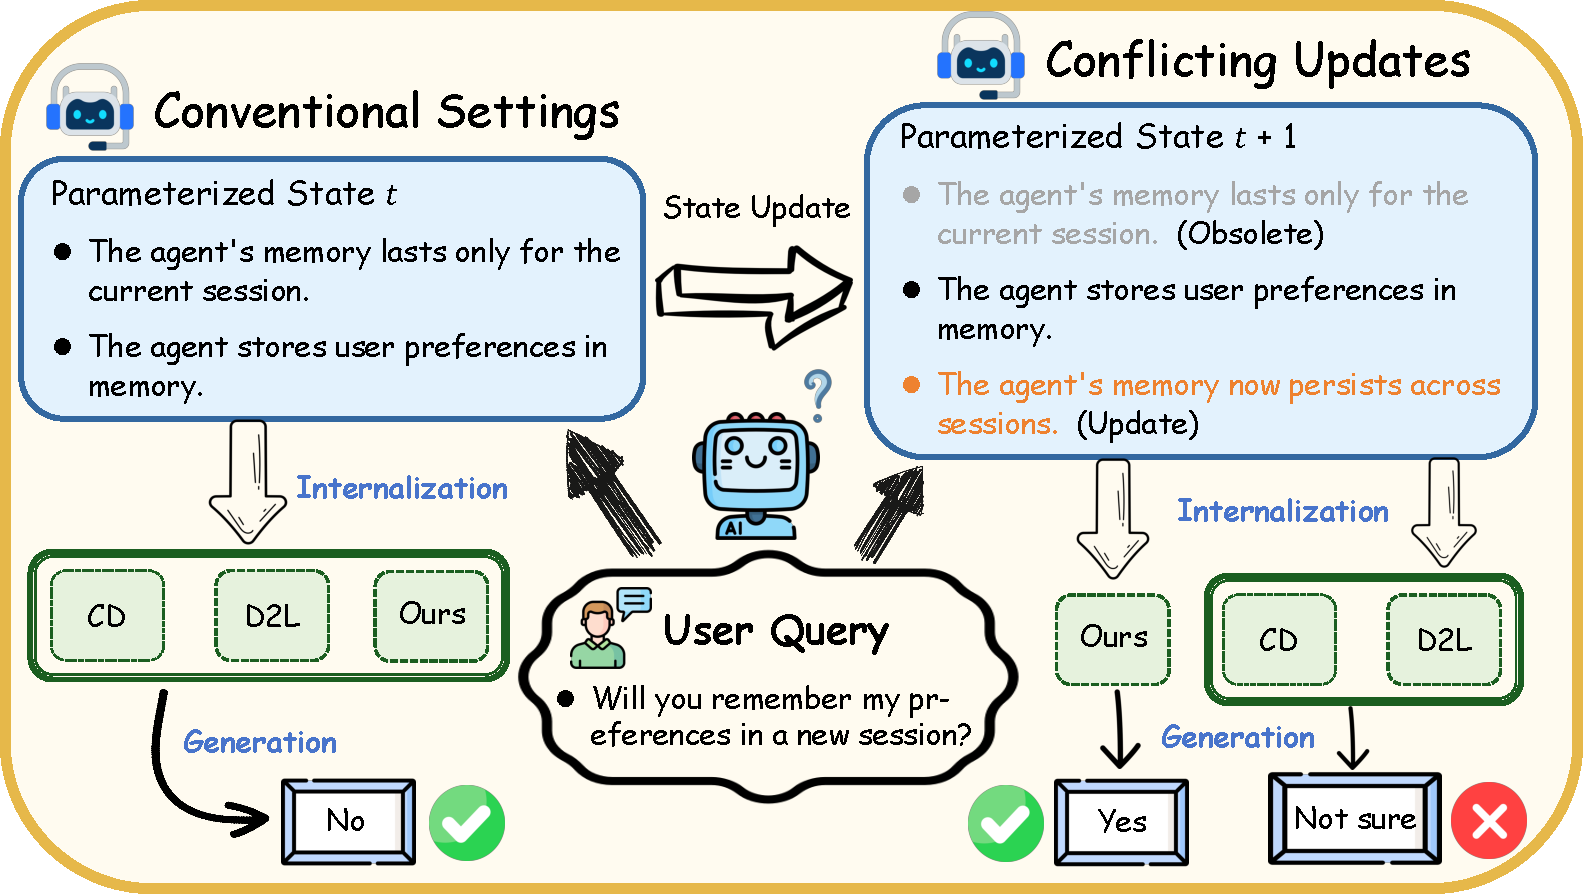
\includegraphics[
        width=\textwidth,
        % trim=14 83 14 84, % left, bottom, right, top
        clip
    ]{fig/intro/intro_quartz_crop.pdf}
    \caption{\textbf{Illustration of context parameterization under continual updates.}
    While existing methods perform well in conventional settings, they may conflate obsolete information with subsequent updates, whereas \method{} follows the currently valid information.
    }
    \label{fig:intro_motivation}
\end{figure*}

% P1
Large Language Models (LLMs) demonstrated remarkable general-purpose capabilities in question answering, reasoning, and text generation, advancing natural language processing~\citep{brown2020language,wei2022chain,guo2025deepseek}. 
Many practical tasks are context-intensive, requiring models to efficiently locate and reuse information from long contexts across successive queries~\citep{bai2024longbench,bai2025longbench,li2025scbench}.
Existing retrieval-augmented generation (RAG)~\citep{lewis2020retrieval,guu2020retrieval} and long-context methods~\citep{ding2023longnet} incur substantial inference overhead from repeated context processing~\citep{gao2023retrieval}, whereas context parameterization decouples this process from subsequent queries, enabling efficient reuse~\citep{snell2022learning,charakorn2026doc}.
Prior research followed two lines: \ding{172} one updated parametric knowledge through localized parameter modifications without retraining the model, as in knowledge editing~\citep{mitchell2022fast,meng2022locating,meng2023massediting}; \ding{173} the other internalized contextual information into reusable parameter representations, as in context distillation, Doc-to-LoRA, and SHINE, which compiled contexts into lightweight representations for subsequent queries~\citep{snell2022learning,charakorn2026doc,liu2026shine}.

% P2
Although these methods enabled effective, efficient context reuse, none addressed parameterization under evolving information validity~\citep{liu2025model,tian2026anyedit}.
In long-running agents and interactive systems, information continuously accumulates into persistent memory, making full context reconstruction impractical~\citep{park2023generative,packer2023memgpt,zhong2024memorybank}, motivating parameterized states that incorporate new information while preserving prior~\citep{jang2022temporalwiki}.
However, under continual updates, some information remains valid while other information is supplemented, replaced, or invalidated~\citep{wallat2026facts}, and jointly retaining information with different validity states can cause reliance on invalid information or inconsistent responses~\citep{marjanovic2024dynamicqa,wallat2026facts}.
Incorporating continual updates into a parameterized state while adhering to valid information thus remains an open challenge, as illustrated in Figure~\ref{fig:intro_motivation}: after an update, the parameterized state must incorporate updates while preserving what remains unaffected.

% P3
To study this continual-update setting, we formalized \textbf{Memory Updating with Sequential Evolution (\task{})} and designed a data construction pipeline preserving the original question and context structures, updating only the target and coupled information, and appending the updated context to the original.
This construction produces a context history with explicit update order and validity changes that supports the updated answer while no longer supporting the previous one.
Using this pipeline, we constructed \benchmark{} from five datasets, covering QA and reasoning.
Unlike prior work on conflicts between external context and model priors~\citep{xie2024adaptive,xu2024knowledge,kortukov2024studying}, \benchmark{} studies continual updates where valid and invalid information coexist within a parameterized state.
Experiments showed that parameterizing the full context into a unified representation substantially degraded performance, indicating severe interference among information with different validity states.

% P4
Building on \benchmark{}, we examined whether interference reflected information loss or merely suppressed activation by computing token-level ROUGE-L recall under teacher forcing for top-1 and top-5 candidate tokens at each step.
Top-5 recall reached \textbf{71.79}\%, far exceeding top-1's \textbf{45.90}\%, indicating valid information was largely retained in the output distribution but frequently outranked by invalid candidates. 
Thus, the observed interference was primarily a ranking rather than an information-loss problem. 
This finding motivates \method{}'s design: since the signal is present but underweighted, we first amplify the global representation; however, suppression varies across queries, so uniform amplification cannot precisely target which candidate to reweight and may override valid information, motivating query-activated memory evidence for precise, per-query correction. 
We retain the global representation rather than relying on local evidence alone because query-activated evidence can fail when a query's phrasing diverges from the original update context, lacking the cross-passage consistency encoded by the global representation. 
\method{} thus adaptively integrates both at decoding time---the global representation as a stable prior and memory evidence as a precise correction.

% P5
Experiments spanned multiple model families, including Qwen3 and Gemma2~\citep{yang2025qwen3,team2024gemma}, on five public state-update datasets, comparing \method{} with knowledge editing~\citep{jiang2025anyedit}, context distillation~\citep{askell2021general,snell2022learning}, Doc-to-LoRA~\citep{charakorn2026doc}, and other representative baselines.
Averaged across the five datasets, \method{} improved ROUGE-L Recall from \textbf{44.46} (D2L) to \textbf{57.76} (\textbf{13.30}$\uparrow$), and LLM-as-a-Judge from \textbf{34.49} to \textbf{53.41} (\textbf{18.92}$\uparrow$), while consistently outperforming all baselines across models and task settings.
These results demonstrated that \method{} effectively mitigated parametric interference among information with different validity states while improving adherence to currently valid information.

\section{Background}
\label{sec:background}

% This paper studies context parameterization under continual updates, where contextual information is internalized into a parameterized state for reuse across queries. 
% Let $C$, $q$, and $y$ denote the context, query, and answer sequences, respectively, and let $p_\theta$ denote the conditional generation distribution of a language model with parameters $\theta$.
% Conventional long-context and RAG methods instead supply context explicitly at inference time, generating answers via $p_\theta(y\mid C,q)$~\citep{lewis2020retrieval,guu2020retrieval,ding2023longnet}.
% This incurs repeated reprocessing overhead per query, and long-context models may further suffer degraded information access depending on context position~\citep{liu2024lost,hsieh2024found}.
We study context parameterization under continual updates, internalizing information into a parameterized state reused across queries as $C$ grows monotonically.
Let $C$, $q$, and $y$ denote the context, query, and answer, and $p_\theta(\cdot\mid\cdot)$ the conditional distribution of a $\theta$-parameterized language model.
Conventional long-context and RAG methods supply context at inference time---concatenating context into the input window or retrieving passages---via $p_\theta(y\mid C,q)$~\citep{lewis2020retrieval,guu2020retrieval,ding2023longnet}, incurring reprocessing costs scaling with $|C|$, compounding across queries~\citep{gao2023retrieval}, and suffering position bias, underutilizing evidence away from the input's boundaries~\citep{liu2024lost,hsieh2024found}.
These costs motivate context parameterization internalizing $C$ into parameters decoupled from per-query inference.

Context Distillation (CD) instead transfers contextual information from explicit input into model parameters.
Given a context $C$ and an associated query distribution $\mathcal{Q}_C$, CD uses a context-conditioned teacher to optimize a context-specific parameter state $\theta_C$:
\begin{equation}
\min_{\theta_C}\mathbb{E}_{q\sim\mathcal{Q}_C}\left[
D_{\mathrm{KL}}\left(p_\theta(\cdot\mid C,q)\parallel
p_{\theta_C}(\cdot\mid q)\right)\right].
\end{equation}
The teacher has direct access to $C$, whereas the student is optimized to reproduce the teacher distribution using only the query.
In this way, information originally supplied through the input context is encoded into the resulting parameter state.
After distillation, the model can answer queries without explicitly receiving $C$ during inference, allowing the same parameterized context to be reused across multiple queries~\citep{askell2021general,snell2022learning}.
However, CD requires context-specific distillation data and iterative optimization for each new context, making repeated updates costly.

Doc-to-LoRA (D2L) amortizes this per-context optimization using a hypernetwork $H_\phi$ that maps a context directly to a LoRA weight delta~\citep{hu2022lora,charakorn2026doc}:
\begin{equation}
\Delta W_C=H_\phi(C),\qquad
\theta_C=\theta\oplus\Delta W_C .
\end{equation}
Here, $\Delta W_C$ denotes the generated LoRA adapter and $\oplus$ denotes applying it to the frozen base model.
Instead of optimizing a separate parameter state for each context, D2L learns the mapping from contextual information to parameter updates across a collection of training contexts.
Once trained, $H_\phi$ generates a reusable context-specific adapter in a single forward pass, substantially reducing the parameterization cost for previously unseen contexts.
The generated adapter can be independently applied to or removed from the frozen base model, providing a lightweight parameter representation of the corresponding context.
However, D2L parameterizes contexts without explicitly modeling continual updates to existing parameterized states.
\section{\benchmark{}}
\label{sec:benchmark}

To systematically evaluate context parameterization under continual updates, we defined the \textbf{\task{} (Memory Updating with Sequential Evolution)} task and constructed \textbf{\benchmark{}}, focusing on incorporating currently valid information while preserving unaffected information.


\subsection{Motivation and Task Formulation}

\paragraph{Motivation.}
Existing context parameterization methods primarily consider contexts to be static and internally consistent, without explicitly considering conflicts introduced by continual updates~\citep{charakorn2026doc,liu2026shine}. 
Prior evaluations primarily assessed either static context internalization~\citep{snell2022learning,charakorn2026doc,liu2026shine} or targeted factual modifications~\citep{meng2022locating,meng2023massediting}, leaving the incorporation of continual updates and the preservation of unaffected information in parameterized representations insufficiently evaluated.
\benchmark{} is designed to address this gap in a unified setting.

\paragraph{Task Formulation.}
Given an original context $C_o$ and a subsequent update context $C_u$, we concatenate them chronologically to form the full context history used for subsequent parameterization
\begin{equation}C_f = C_o \Vert C_u,\end{equation}
where later information in $C_u$ determines the currently valid state of updated facts, while unaffected information remains unchanged. 
Let $\mathcal{A}$ denote a context parameterization method that transforms $C_f$ into a context-specific parameter state:
\begin{equation}
\theta_f = \mathcal{A}(\theta, C_f),
\label{eq:context-parameterization}
\end{equation}
where $\theta$ denotes the base model parameters. After parameterization, the model receives only the query $q$ and generates
\begin{equation}
\hat{y}(q) = \operatorname*{arg\,max}_{y} p_{\theta_f}(y\mid q).
\label{eq:muse-inference}
\end{equation}
Let $y^\star(q)$ denote the reference answer determined by the currently valid information in $C_f$. 
We divide queries into two categories: $\mathcal{Q}_{\mathrm{upd}}$, whose answers are affected by the update, and $\mathcal{Q}_{\mathrm{keep}}$, whose answers remain unchanged. 
Both categories are evaluated under the parameterized full context history, although $\mathcal{Q}_{\mathrm{keep}}$ remains answerable from unaffected information in $C_o$. \task{} evaluates whether the parameterized state incorporates updated information while preserving unaffected answers.


\subsection{Benchmark Construction}
\label{sec:benchmark-dataset}

\benchmark{} comprises five datasets: SQuAD, ROPES, 2WikiMultihopQA, MultiFieldQA-en, and QASPER~\citep{rajpurkar2016squad,lin2019reasoning,ho2020constructing,bai2024longbench,dasigi2021dataset}, with approximately \textbf{3,000 contexts} and \textbf{13,000 question-answer pairs} in total.
Given an original context $C_o=\{c_1,c_2,\ldots,c_n\}$, we randomly sampled evidence units supporting a target answer and carefully updated the corresponding facts while preserving the original question and context structures. When other facts had semantic or reasoning dependencies on the target facts, we updated them consistently to construct an internally coherent update context $C_u$, which was then appended to $C_o$ to form the full context history $C_f$. The resulting context history supports the currently valid answers for update-affected queries while preserving the corresponding original answers for unaffected queries.


Candidate samples were generated with GPT-series models for fact modification, dependency identification, and question-answer annotation, primarily using GPT-5.5~\citep{openai2026gpt55} and GPT-5.6-Sol~\citep{openai2026gpt56} throughout the benchmark construction process.
We further used GPT-5.6-Sol to conduct 26 rounds of quality verification, checking:
(1) whether $C_f$ supports the current correct answers;
(2) whether coupled information are consistently updated; and
(3) whether unaffected answers remain supported by $C_f$.
Detailed construction procedures, annotation prompts, and quality control protocols are provided in Appendix~\ref{app:annotation-guidelines}.



\subsection{Evaluation Protocol}
\label{sec:benchmark-evaluation}

\benchmark{} evaluates model outputs from four complementary perspectives of answer quality and update robustness.
\textbf{\rule[0.1em]{0.45em}{0.45em}\hspace{0.3em}D1 Answer Coverage}
uses token-level ROUGE-L Recall~\citep{lin2004rouge} to measure reference-answer coverage.
\textbf{\rule[0.1em]{0.45em}{0.45em}\hspace{0.3em}D2 Semantic Equivalence}
evaluates whether the generated answer is semantically equivalent to the current reference answer.
\textbf{\rule[0.1em]{0.45em}{0.45em}\hspace{0.3em}D3 Final-Answer Agreement}
measures whether the model's final answer agrees with the reference answer.
\textbf{\rule[0.1em]{0.45em}{0.45em}\hspace{0.3em}D4 Locality}
measures whether the model preserves correct answers for queries unaffected by the update.
Together, these metrics evaluate both effective incorporation of currently valid information and reliable preservation of unaffected information.

All metrics are computed at the query level and then aggregated within each dataset for overall performance comparison.
For D2 and D3, we used \textbf{GPT-5.6-Sol} as the LLM Judge with unified evaluation prompts and consistent evaluation criteria.
Detailed evaluation settings and complete evaluation rubrics are provided in Appendix~\ref{app:evaluation-setup}.

% \section{Method}
% \label{sec:method}

% We propose \textbf{Parametric LoRA Updates with Memory Evidence (\method{})}.
% \method{} constructs a global update LoRA to preserve the full context state while emphasizing the latest update, activates query-relevant memory evidence to provide a local parameter view, and adaptively incorporates this local evidence during decoding.

% Figure~\ref{fig:method-overview} provides an overview of the complete \method{} pipeline.
% The upper branch constructs the global update state from the parameter difference between the pre-update and full contexts, while the lower branch activates and parameterizes query-relevant memory evidence.
% Their predictive distributions are combined during adaptive decoding to emphasize currently valid information while retaining unaffected knowledge.

% \begin{figure*}[t]
%     \centering
%     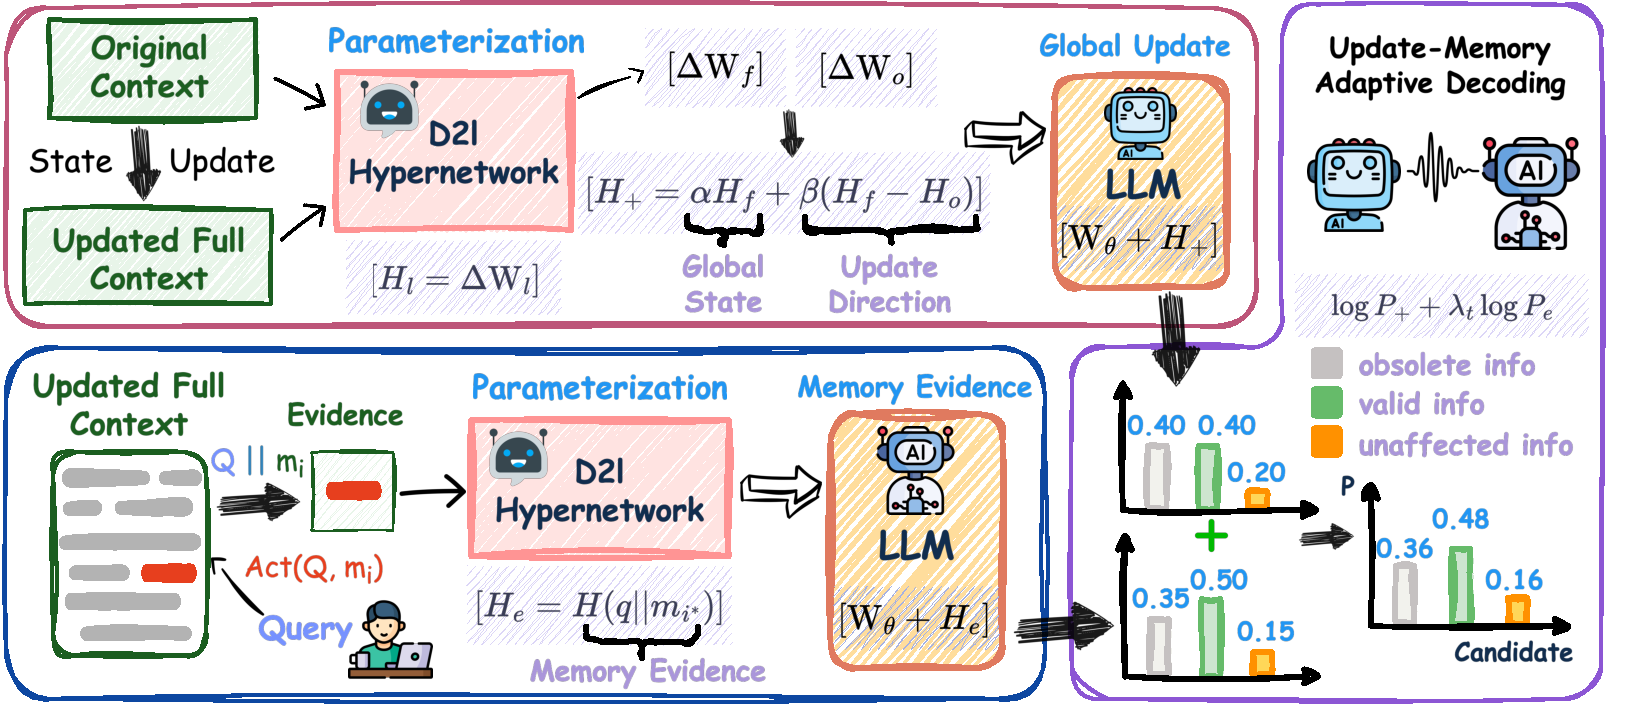
\includegraphics[width=\textwidth]{fig/intro/method.pdf}
%     \caption{Overview of \method{}. The global branch models the parameter change induced by the latest context update, while the memory-evidence branch constructs a query-relevant local parameter view. Adaptive decoding combines their predictions according to the evidence-induced prediction change.}
%     \label{fig:method-overview}
% \end{figure*}


% \subsection{\gur{}}
% \label{sec:global_update_backbone}

% Under continual context updates, a parameterized context may simultaneously encode currently valid, invalidated, and unaffected information.
% To emphasize the latest update while preserving the full context state, we explicitly model the parameter change before and after the update.

% Given the full context history $C_{\mathrm{full}}$ and its pre-update state $C_{\mathrm{old}}$, we parameterize both using the context parameterization hypernetwork $H_\phi$ introduced in Section~\ref{sec:background}, obtaining $\Delta W_{\mathrm{old}}=H_\phi(C_{\mathrm{old}})$ and $\Delta W_{\mathrm{full}}=H_\phi(C_{\mathrm{full}})$.

% Directly using $\Delta W_{\mathrm{full}}$ preserves the complete context history, but may mix information with different validity states.
% In contrast, the difference between the parameter states before and after the update explicitly captures the parameter change induced by the latest update.
% We therefore construct the global update LoRA as
% \begin{equation}
% \Delta W_g
% =
% \alpha \Delta W_{\mathrm{full}}
% +
% \beta
% \left(
% \Delta W_{\mathrm{full}}
% -
% \Delta W_{\mathrm{old}}
% \right),
% \label{eq:global_adapter}
% \end{equation}
% where $\alpha,\beta \geq 0$ are weighting coefficients.
% The first term preserves the overall information encoded by the full context history, while the second amplifies the parameter change induced by the latest update, thereby emphasizing the update direction.

% After applying $\Delta W_g$ to the frozen base model, the global predictive distribution at the $t$-th generation step is
% \begin{equation}
% p_{g,t}(v)
% =
% p_{\theta \oplus \Delta W_g}
% \left(
% v \mid q, y_{<t}
% \right),
% \label{eq:global-distribution}
% \end{equation}
% where $v$ denotes a candidate token, $y_{<t}$ is the previously generated prefix, and $\oplus$ denotes applying the corresponding LoRA adapter to the frozen base model.


% \subsection{\qame{}}
% \label{sec:memory_evidence_activation}

% Although the global update LoRA preserves the full context state, each query typically depends on only a subset of the information contained in the context.
% Relying solely on a unified global parameter state may therefore still introduce interference from information irrelevant to the current query.

% To provide a query-specific local parameter view, we segment $C_{\mathrm{full}}$ into memory units and score each unit according to its lexical relevance to the query.
% The activation score combines query-term coverage with saturated term-frequency matching.
% We select the highest-scoring memory unit as the local memory evidence for the current query, denoted by $m^\star(q)$.
% The query is used only to activate relevant memory evidence and is not passed to the context parameterization hypernetwork.

% We then parameterize the activated memory evidence into an evidence LoRA:
% \begin{equation}
% \Delta W_e(q)
% =
% H_\phi
% \left(
% m^\star(q)
% \right).
% \label{eq:evidence_adapter}
% \end{equation}

% This yields the query-conditioned evidence distribution
% \begin{equation}
% p_{e,t}(v)
% =
% p_{\theta \oplus \Delta W_e(q)}
% \left(
% v \mid q, y_{<t}
% \right).
% \label{eq:evidence-distribution}
% \end{equation}

% Unlike the global LoRA, which encodes the full context history, $\Delta W_e(q)$ captures only the local memory evidence activated for the current query.
% This provides a focused parameter view that emphasizes information directly relevant to the current prediction while reducing interference from unrelated context.


% \subsection{\amd{}}
% \label{sec:adaptive_evidence_decoding}

% The global distribution $p_{g,t}$ provides the complete context state, whereas the evidence distribution $p_{e,t}$ emphasizes local information relevant to the current query.
% However, the contribution of local evidence may vary across generation steps.
% When the local evidence produces predictions similar to the global state, the global prediction is generally sufficient; when it substantially changes the prediction, the local evidence should contribute more strongly.

% We therefore measure the prediction change induced by the local memory evidence using the Jensen--Shannon divergence between the evidence and global distributions:
% \begin{equation}
% d_t
% =
% D_{\mathrm{JS}}
% \left(
% p_{e,t}
% \parallel
% p_{g,t}
% \right).
% \label{eq:js-divergence}
% \end{equation}

% We then convert this divergence into an adaptive evidence weight:
% \begin{equation}
% \lambda_t
% =
% \lambda_{\max}
% \frac{
% d_t
% }{
% d_t+\tau
% },
% \label{eq:adaptive_gate}
% \end{equation}
% where $\lambda_{\max}$ controls the maximum contribution of local evidence and $\tau>0$ controls how rapidly the evidence weight increases with the prediction change.
% A larger divergence results in a larger $\lambda_t$, while similar global and evidence distributions lead to a smaller contribution from the local evidence.

% Finally, we retain the global prediction as the decoding backbone and adaptively augment it with the local evidence prediction:
% \begin{equation}
% S_t(v)
% =
% \log p_{g,t}(v)
% +
% \lambda_t
% \log p_{e,t}(v),
% \label{eq:fusion-score}
% \end{equation}
% where $S_t(v)$ denotes the fused score for token $v$.
% The token with the highest fused score is selected at each generation step.
































% \section{Method}
% \label{sec:method}

% \begin{figure*}[t]
%     \centering
%     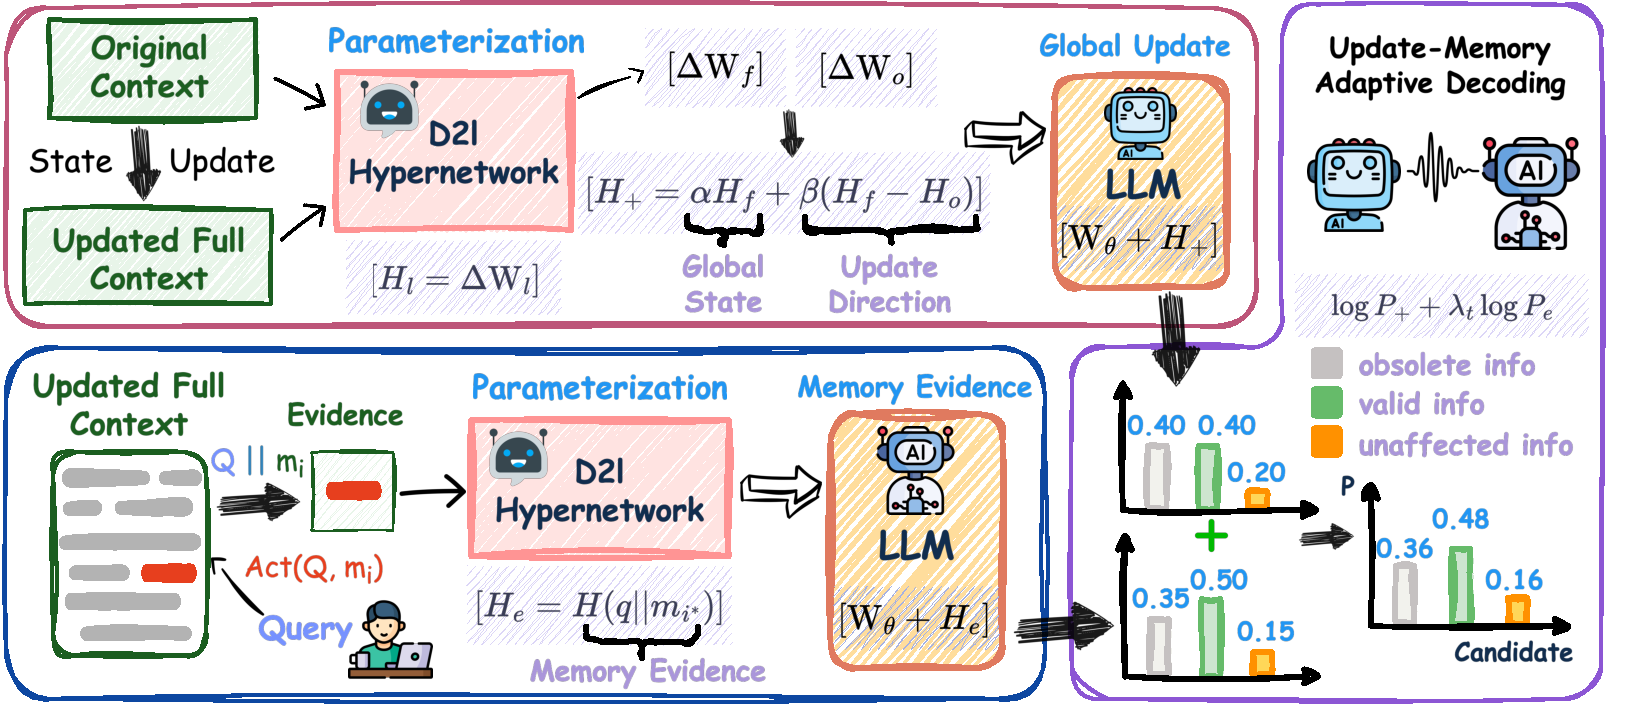
\includegraphics[width=\textwidth]{fig/intro/method.pdf}
%     \captionsetup{justification=raggedright,singlelinecheck=false}
%     \caption{\textbf{The overall framework of our proposed \method{}.}}
%     \label{fig:method-overview}
% \end{figure*}

% We propose \textbf{Parametric LoRA Updates with Memory Evidence (\method{})}.
% \method{} constructs a global update LoRA that preserves the full context state while emphasizing the latest update, activates query-relevant memory evidence as a local parameter view, and adaptively integrates the two during decoding.

% Figure~\ref{fig:method-overview} illustrates the overall pipeline.
% The global branch models the parameter change between the pre-update and full contexts, while the memory-evidence branch parameterizes query-relevant local information.
% Their predictive distributions are adaptively combined to favor currently valid information while preserving unaffected knowledge.



% \subsection{\gur{}}
% \label{sec:global_update_backbone}

% Under continual updates, a parameterized context may simultaneously encode currently valid, invalidated, and unaffected information.
% We therefore model the parameter change induced by the latest update while retaining the full context state.

% Given the full context history $C_{\mathrm{full}}$ and its pre-update state $C_{\mathrm{old}}$, we parameterize both using the context parameterization hypernetwork $H_\phi$ introduced in Section~\ref{sec:background}:
% $\Delta W_{\mathrm{old}}=H_\phi(C_{\mathrm{old}})$ and
% $\Delta W_{\mathrm{full}}=H_\phi(C_{\mathrm{full}})$.

% We construct the global update LoRA as
% \begin{equation}
% \Delta W_g
% =
% \alpha \Delta W_{\mathrm{full}}
% +
% \beta
% \left(
% \Delta W_{\mathrm{full}}
% -
% \Delta W_{\mathrm{old}}
% \right),
% \label{eq:global_adapter}
% \end{equation}
% where $\alpha,\beta \geq 0$ are weighting coefficients.
% The first term preserves the full context state, while the second emphasizes the parameter change induced by the latest update.

% The resulting global predictive distribution at generation step $t$ is
% \begin{equation}
% p_{g,t}(v)
% =
% p_{\theta \oplus \Delta W_g}
% \left(
% v \mid q, y_{<t}
% \right),
% \label{eq:global-distribution}
% \end{equation}
% where $v$ is a candidate token, $y_{<t}$ is the generated prefix, and $\oplus$ denotes applying the LoRA adapter to the frozen base model.


% \subsection{\qame{}}
% \label{sec:memory_evidence_activation}

% A query typically depends on only a subset of the full context, so a unified global parameter state may introduce interference from irrelevant information.
% We therefore construct a query-specific local parameter view.

% We segment $C_{\mathrm{full}}$ into memory units and score them by lexical relevance to the query using query-term coverage and saturated term-frequency matching.
% The highest-scoring unit is selected as the local memory evidence $m^\star(q)$.
% The query is used only for evidence activation and is not passed to the context parameterization hypernetwork.

% The activated evidence is parameterized as
% \begin{equation}
% \Delta W_e(q)
% =
% H_\phi
% \left(
% m^\star(q)
% \right),
% \label{eq:evidence_adapter}
% \end{equation}
% yielding the evidence distribution
% \begin{equation}
% p_{e,t}(v)
% =
% p_{\theta \oplus \Delta W_e(q)}
% \left(
% v \mid q, y_{<t}
% \right).
% \label{eq:evidence-distribution}
% \end{equation}

% Unlike the global LoRA, $\Delta W_e(q)$ captures only query-relevant local evidence, providing a more focused parameter view for the current prediction.

% % Queue the main results table after page 5's top floats have been placed,
% % so that it appears at the top of page 6 before the experiments section.
% % \begingroup

% \definecolor{headerbg}{HTML}{FAF7FF}

% \definecolor{recallarrow}{HTML}{F05A3C}

% \definecolor{llmarrow}{HTML}{3182CE}

% \newcommand{\RecallMetric}{Recall\,\textcolor{recallarrow}{$\uparrow$}}

% \newcommand{\LLMMetric}{LLM\,\textcolor{llmarrow}{$\uparrow$}}

% \newcommand{\PLUMENumber}[1]{{\color{black}\bfseries #1}}

% \newcommand{\SecondNumber}[1]{\uline{#1}}

% \newcommand{\MethodFont}{\fontsize{12pt}{34pt}\selectfont\bfseries}

% \newlength{\ModelHeadingOffset}

% \newlength{\ModelHeadingHeight}

% \newlength{\ModelHeadingAboveSep}

% \newlength{\ModelHeadingBelowSep}

% \setlength{\ModelHeadingOffset}{10.1cm}

% \setlength{\ModelHeadingHeight}{8pt}

% \setlength{\ModelHeadingAboveSep}{0pt}

% \setlength{\ModelHeadingBelowSep}{0pt}

% \newcommand{\ModelHeadingText}[1]{%
%   \makebox[0pt][l]{\hspace*{\ModelHeadingOffset}%
%     {\color{gray}\itshape #1}}%
% }

% \newcommand{\DatasetHeader}[1]{%
%   \begin{tblr}{
%       colspec={Q[c,wd=1.35cm]Q[c,wd=1.05cm]},
%       colsep=3.1pt,
%       rowsep=2pt,
%       rows={font=\bfseries,halign=c,valign=m},
%       hline{2}={wd=0.5pt,solid,leftpos=-0.5,rightpos=-0.5},
%     }
%     \SetCell[c=2]{halign=c,valign=m}#1 & {} \\
%     \RecallMetric & \LLMMetric
%   \end{tblr}%
% }

% \begin{table*}[t]

% \centering

% \small

% \caption{\textbf{Performance comparison of different methods} on five MUSE-Bench datasets across Qwen3 and Gemma-2, evaluated by ROUGE-L Recall and LLM-as-a-Judge.}

% \label{tab:main_results}

% \resizebox{\textwidth}{!}{%

% \begin{tblr}{
%     colspec = {
%         Q[l,wd=4.6cm,valign=m]
%         *{5}{
%             Q[c,wd=1.35cm,valign=m]
%             Q[c,wd=1.05cm,valign=m]
%         }
%     },
%     rowsep = 1pt,
%     % Keep the two rules above each PLUME row distinct after resizing.
%     rulesep = 2pt,
%     colsep = 4pt,
%     row{1} = {bg=headerbg, halign=c, valign=m, font=\bfseries,
%               abovesep=2pt, belowsep=2pt},
%     hline{1} = {wd=2pt, solid},
%     hline{2,11} = {wd=2pt, solid},
%     % The PLUME rows are rows 10 and 19.  Number the two rules explicitly
%     % on those boundaries so they cannot attach to the preceding data row.
%     hline{10,19} = {1}{-}{wd=0.5pt, solid},
%     hline{10,19} = {2}{-}{wd=0.5pt, solid},
%     column{1} = {font=\bfseries},
% }

% \SetCell{halign=c,valign=m}{{\MethodFont Method}}

% & \SetCell[c=2]{halign=c,valign=m}{\DatasetHeader{SQuAD}} & {}

% & \SetCell[c=2]{halign=c,valign=m}{\DatasetHeader{ROPES}} & {}

% & \SetCell[c=2]{halign=c,valign=m}{\DatasetHeader{2Wiki}} & {}

% & \SetCell[c=2]{halign=c,valign=m}{\DatasetHeader{MFQA}} & {}

% & \SetCell[c=2]{halign=c,valign=m}{\DatasetHeader{QASPER}} & {} \\

% \SetRow{ht=\ModelHeadingHeight,
%         abovesep=\ModelHeadingAboveSep,
%         belowsep=\ModelHeadingBelowSep}
% \SetCell[c=11]{halign=l,valign=m}{\ModelHeadingText{Qwen-3}} \\

% \SetHline{1-11}{0.5pt,solid}

% Base Model w/ Context

% & 95.86 & 91.69

% & 97.82 & 95.91

% & 60.11 & 52.35

% & 64.50 & 60.08

% & 61.75 & 53.95

% \\

% Base Model w/o Context

% & 24.61 & 15.19

% & 82.88 & 64.99

% & 31.75 & 24.67

% & 22.48 & 11.33

% & 1.28 & 1.89

% \\

% CD (oracle)

% & 94.93 & 91.75

% & 98.31 & 97.52

% & 68.51 & 65.44

% & 66.24 & 61.17

% & 62.46 & 55.81

% \\

% D2L (oracle)

% & 76.77 & 64.92

% & 85.57 & 80.39

% & 43.13 & 38.33

% & 28.80 & 20.34

% & 22.98 & 15.80

% \\

% CD

% & 40.57 & 27.85

% & 74.69 & 67.00

% & 36.15 & 30.67

% & \SecondNumber{30.78} & \SecondNumber{23.33}

% & 16.78 & 9.57

% \\

% D2L

% & \SecondNumber{54.96} & \SecondNumber{37.27}

% & \SecondNumber{86.99} & \SecondNumber{81.33}

% & \SecondNumber{36.30} & \SecondNumber{30.84}

% & 27.15 & 12.00

% & \SecondNumber{16.88} & \SecondNumber{11.02}

% \\

% AnyEdit (AlphaEdit)

% & 15.77 & 12.44

% & 76.43 & 67.48

% & 16.25 & 15.00

% & 13.23 & 9.25

% & 7.40 & 4.02

% \\

% \SetRow{font=\bfseries\color{black}}

% PLUME

% & \PLUMENumber{80.65} & \PLUMENumber{76.81}

% & \PLUMENumber{94.61} & \PLUMENumber{90.26}

% & \PLUMENumber{47.24} & \PLUMENumber{41.48}

% & \PLUMENumber{37.76} & \PLUMENumber{34.01}

% & \PLUMENumber{28.53} & \PLUMENumber{24.48}

% \\

% \SetRow{ht=\ModelHeadingHeight,
%         abovesep=\ModelHeadingAboveSep,
%         belowsep=\ModelHeadingBelowSep}
% \SetCell[c=11]{halign=l,valign=m}{\ModelHeadingText{Gemma-2}} \\

% \SetHline{1-11}{0.5pt,solid}

% Base Model w/ Context

% & 90.73 & 84.65

% & 84.73 & 80.17

% & 36.39 & 28.21

% & 31.81 & 27.49

% & 52.48 & 44.72

% \\

% Base Model w/o Context

% & 22.07 & 12.54

% & 44.44 & 25.95

% & 14.76 & 6.49

% & 5.02 & 3.36

% & 0.95 & 1.17

% \\

% CD (oracle)

% & 89.92 & 84.77

% & 85.81 & 79.38

% & 42.23 & 34.39

% & 35.11 & 30.84

% & 52.46 & 45.40

% \\

% D2L (oracle)

% & 70.81 & 57.46

% & 58.84 & 50.43

% & 22.11 & 16.15

% & 14.75 & 7.72

% & 19.10 & 12.58

% \\

% CD

% & 32.30 & 20.19

% & 54.63 & 45.21

% & 20.82 & 14.48

% & 9.72 & \SecondNumber{6.76}

% & 12.94 & 5.23

% \\

% D2L

% & \SecondNumber{49.17} & \SecondNumber{31.36}

% & \SecondNumber{57.53} & \SecondNumber{48.69}

% & \SecondNumber{21.09} & \SecondNumber{15.96}

% & \SecondNumber{11.44} & 6.55

% & \SecondNumber{14.22} & \SecondNumber{7.96}

% \\

% AnyEdit (AlphaEdit)

% & 16.24 & 8.93

% & 51.81 & 41.72

% & 10.37 & 8.64

% & 5.23 & 4.06

% & 0.54 & 0.46

% \\

% \SetRow{font=\bfseries\color{black}}

% PLUME

% & \PLUMENumber{74.80} & \PLUMENumber{68.60}

% & \PLUMENumber{62.70} & \PLUMENumber{55.78}

% & \PLUMENumber{29.85} & \PLUMENumber{24.82}

% & \PLUMENumber{23.29} & \PLUMENumber{19.42}

% & \PLUMENumber{24.51} & \PLUMENumber{20.35}

% \\

% \SetHline{1-11}{2pt,solid}

% \end{tblr}%

% }

% \end{table*}

% \endgroup


\begingroup

\definecolor{headerbg}{HTML}{FAF7FF}

\definecolor{recallarrow}{HTML}{F05A3C}

\definecolor{llmarrow}{HTML}{3182CE}

\newcommand{\RecallMetric}{Recall\,\textcolor{recallarrow}{$\uparrow$}}

\newcommand{\LLMMetric}{LLM\,\textcolor{llmarrow}{$\uparrow$}}

\newcommand{\PLUMENumber}[1]{{\color{black}\bfseries #1}}

\newcommand{\SecondNumber}[1]{\uline{#1}}

\newcommand{\MethodFont}{\fontsize{12pt}{34pt}\selectfont\bfseries}

\newlength{\ModelHeadingOffset}

\newlength{\ModelHeadingHeight}

\newlength{\ModelHeadingAboveSep}

\newlength{\ModelHeadingBelowSep}

\setlength{\ModelHeadingOffset}{10.1cm}

\setlength{\ModelHeadingHeight}{8pt}

\setlength{\ModelHeadingAboveSep}{0pt}

\setlength{\ModelHeadingBelowSep}{0pt}

\newcommand{\ModelHeadingText}[1]{%
  \makebox[0pt][l]{\hspace*{\ModelHeadingOffset}%
    {\color{gray}\itshape #1}}%
}

\newcommand{\DatasetHeader}[1]{%
  \begin{tblr}{
      colspec={Q[c,wd=1.35cm]Q[c,wd=1.05cm]},
      colsep=3.1pt,
      rowsep=2pt,
      rows={font=\bfseries,halign=c,valign=m},
      hline{2}={wd=0.5pt,solid,leftpos=-0.5,rightpos=-0.5},
    }
    \SetCell[c=2]{halign=c,valign=m}#1 & {} \\
    \RecallMetric & \LLMMetric
  \end{tblr}%
}

\begin{table*}[t]

\centering

\small

\caption{\textbf{Performance comparison of different methods} on five MUSE-Bench datasets across Qwen3 and Gemma-2, evaluated by ROUGE-L Recall and LLM-as-a-Judge. Oracle methods are excluded when identifying the best and second-best methods.}

\label{tab:main_results}

\resizebox{\textwidth}{!}{%

\begin{tblr}{
    colspec = {
        Q[l,wd=4.6cm,valign=m]
        *{5}{
            Q[c,wd=1.35cm,valign=m]
            Q[c,wd=1.05cm,valign=m]
        }
    },
    rowsep = 1pt,
    % Keep the two rules above each PLUME row distinct after resizing.
    rulesep = 2pt,
    colsep = 4pt,
    row{1} = {bg=headerbg, halign=c, valign=m, font=\bfseries,
              abovesep=2pt, belowsep=2pt},
    hline{1} = {wd=2pt, solid},
    hline{2,11} = {wd=2pt, solid},
    % The PLUME rows are rows 10 and 19.  Number the two rules explicitly
    % on those boundaries so they cannot attach to the preceding data row.
    hline{10,19} = {1}{-}{wd=0.5pt, solid},
    hline{10,19} = {2}{-}{wd=0.5pt, solid},
    column{1} = {font=\bfseries},
}

\SetCell{halign=c,valign=m}{{\MethodFont Method}}

& \SetCell[c=2]{halign=c,valign=m}{\DatasetHeader{SQuAD}} & {}

& \SetCell[c=2]{halign=c,valign=m}{\DatasetHeader{ROPES}} & {}

& \SetCell[c=2]{halign=c,valign=m}{\DatasetHeader{2Wiki}} & {}

& \SetCell[c=2]{halign=c,valign=m}{\DatasetHeader{MFQA}} & {}

& \SetCell[c=2]{halign=c,valign=m}{\DatasetHeader{QASPER}} & {} \\

\SetRow{ht=\ModelHeadingHeight,
        abovesep=\ModelHeadingAboveSep,
        belowsep=\ModelHeadingBelowSep}
\SetCell[c=11]{halign=l,valign=m}{\ModelHeadingText{Qwen-3}} \\

\SetHline{1-11}{0.5pt,solid}

Base w/ Context (oracle)

& 95.86 & 91.69

& 97.82 & 95.91

& 60.11 & 52.35

& 64.50 & 60.08

& 61.75 & 53.95

\\

CD (oracle)

& 94.93 & 91.75

& 98.31 & 97.52

& 68.51 & 65.44

& 66.24 & 61.17

& 62.46 & 55.81

\\

D2L (oracle)

& 76.77 & 64.92

& 85.57 & 80.39

& 43.13 & 38.33

& 28.80 & 20.34

& 22.98 & 15.80

\\

\SetHline{1-11}{0.5pt,solid}

Base w/o Context

& 24.61 & 15.19

& 82.88 & 64.99

& 31.75 & 24.67

& 22.48 & 11.33

& 1.28 & 1.89

\\

AnyEdit

& 15.77 & 12.44

& 76.43 & 67.48

& 16.25 & 15.00

& 13.23 & 9.25

& 7.40 & 4.02

\\

CD

& 40.57 & 27.85

& 74.69 & 67.00

& 36.15 & 30.67

& \SecondNumber{30.78} & \SecondNumber{23.33}

& 16.78 & 9.57

\\

D2L

& \SecondNumber{54.96} & \SecondNumber{37.27}

& \SecondNumber{86.99} & \SecondNumber{81.33}

& \SecondNumber{36.30} & \SecondNumber{30.84}

& 27.15 & 12.00

& \SecondNumber{16.88} & \SecondNumber{11.02}

\\

\SetRow{font=\bfseries\color{black}}

PLUME

& \PLUMENumber{80.65} & \PLUMENumber{76.81}

& \PLUMENumber{94.61} & \PLUMENumber{90.26}

& \PLUMENumber{47.24} & \PLUMENumber{41.48}

& \PLUMENumber{37.76} & \PLUMENumber{34.01}

& \PLUMENumber{28.53} & \PLUMENumber{24.48}

\\

\SetRow{ht=\ModelHeadingHeight,
        abovesep=\ModelHeadingAboveSep,
        belowsep=\ModelHeadingBelowSep}
\SetCell[c=11]{halign=l,valign=m}{\ModelHeadingText{Gemma-2}} \\

\SetHline{1-11}{0.5pt,solid}

Base w/ Context (oracle)

& 90.73 & 84.65

& 84.73 & 80.17

& 36.39 & 28.21

& 31.81 & 27.49

& 52.48 & 44.72

\\

CD (oracle)

& 89.92 & 84.77

& 85.81 & 79.38

& 42.23 & 34.39

& 35.11 & 30.84

& 52.46 & 45.40

\\

D2L (oracle)

& 70.81 & 57.46

& 58.84 & 50.43

& 22.11 & 16.15

& 14.75 & 7.72

& 19.10 & 12.58

\\

\SetHline{1-11}{0.5pt,solid}

Base w/o Context

& 22.07 & 12.54

& 44.44 & 25.95

& 14.76 & 6.49

& 5.02 & 3.36

& 0.95 & 1.17

\\

AnyEdit

& 16.24 & 8.93

& 51.81 & 41.72

& 10.37 & 8.64

& 5.23 & 4.06

& 0.54 & 0.46

\\

CD

& 32.30 & 20.19

& 54.63 & 45.21

& 20.82 & 14.48

& 9.72 & \SecondNumber{6.76}

& 12.94 & 5.23

\\

D2L

& \SecondNumber{49.17} & \SecondNumber{31.36}

& \SecondNumber{57.53} & \SecondNumber{48.69}

& \SecondNumber{21.09} & \SecondNumber{15.96}

& \SecondNumber{11.44} & 6.55

& \SecondNumber{14.22} & \SecondNumber{7.96}

\\

\SetRow{font=\bfseries\color{black}}

PLUME

& \PLUMENumber{74.80} & \PLUMENumber{68.60}

& \PLUMENumber{62.70} & \PLUMENumber{55.78}

& \PLUMENumber{29.85} & \PLUMENumber{24.82}

& \PLUMENumber{23.29} & \PLUMENumber{19.42}

& \PLUMENumber{24.51} & \PLUMENumber{20.35}

\\

\SetHline{1-11}{2pt,solid}

\end{tblr}%

}

\end{table*}

\endgroup



% \subsection{\amd{}}
% \label{sec:adaptive_evidence_decoding}

% The global distribution $p_{g,t}$ preserves the full context state, whereas $p_{e,t}$ emphasizes query-relevant local evidence.
% Because the usefulness of local evidence may vary across generation steps, we adapt its contribution according to the prediction change it induces.

% We measure this change using the Jensen--Shannon divergence:
% \begin{equation}
% d_t=D_{\mathrm{JS}}\left(p_{e,t}\parallelp_{g,t}\right).
% \label{eq:js-divergence}
% \end{equation}

% The adaptive evidence weight is then
% \begin{equation}
% \lambda_t = \lambda_{\max} \frac{d_t}{d_t+\tau},
% \label{eq:adaptive_gate}
% \end{equation}
% where $\lambda_{\max}$ controls the maximum evidence contribution and $\tau>0$ controls its sensitivity to prediction changes.

% Finally, we retain the global prediction as the decoding backbone and augment it with the local evidence:
% \begin{equation}
% S_t(v) = \log p_{g,t}(v) + \lambda_t \log p_{e,t}(v),
% \label{eq:fusion-score}
% \end{equation}
% where $S_t(v)$ is the fused score for token $v$.
% The token with the highest fused score is selected at each generation step.


\section{Method}
\label{sec:method}

\begin{figure*}[t]
    \centering
    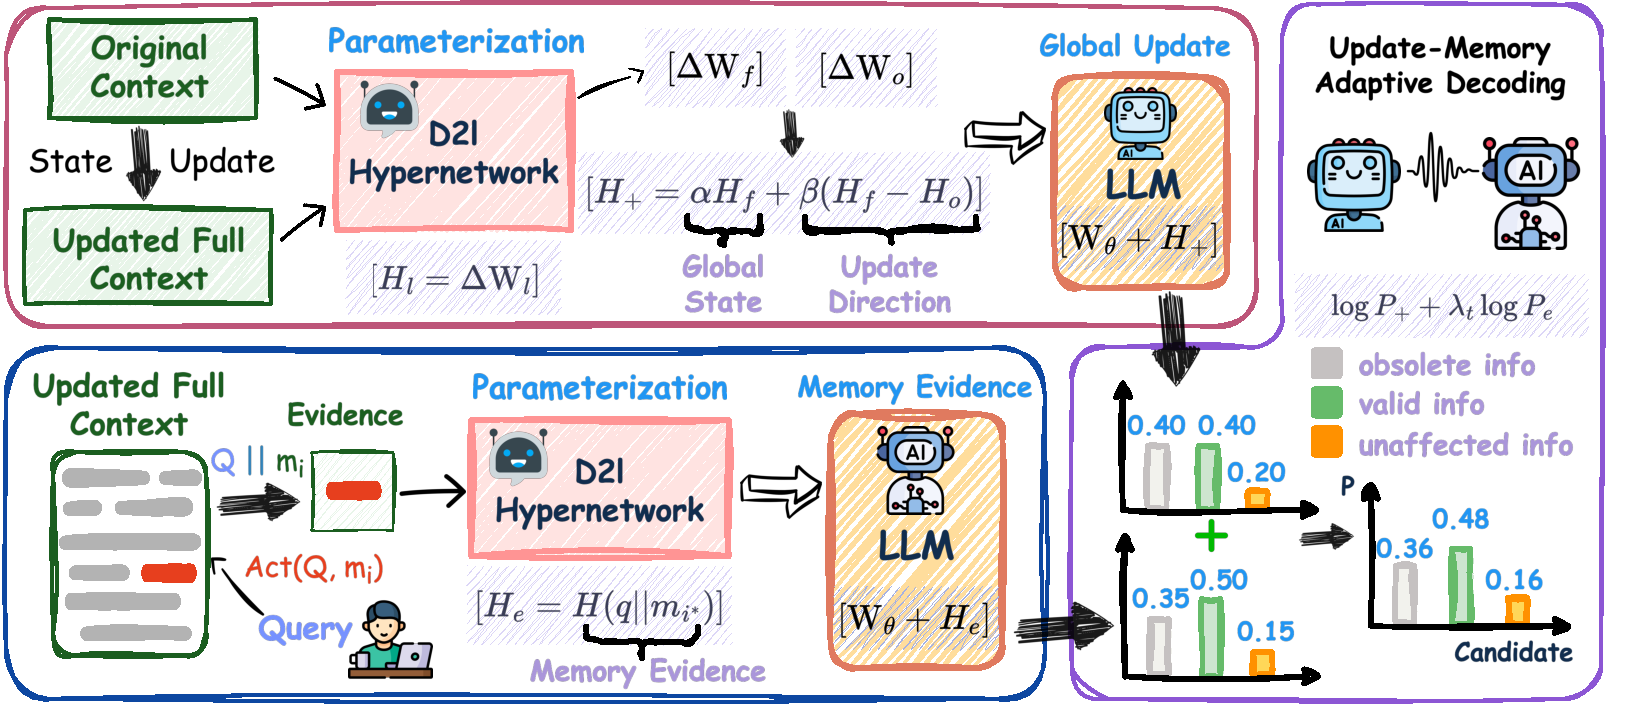
\includegraphics[
        width=\textwidth,
        trim=0 0 15 0,
        clip
    ]{fig/intro/method.pdf}
    \captionsetup{justification=raggedright,singlelinecheck=false}
    \caption{\textbf{The overall framework of our proposed \method{}.} \method{} constructs a global update representation from the full context state, activates memory evidence according to the query to provide a local parameter view, and adaptively integrates the global and local predictions during decoding.
    }
    \label{fig:method-overview}
\end{figure*}

We proposed \textbf{Parametric LoRA Updates with Memory Evidence (\method{})}, which combines a global update representation, query-activated memory evidence, and adaptive decoding for context parameterization under continual updates. Figure~\ref{fig:method-overview} illustrates the overall framework.

\subsection{Global Update Representation}
\label{sec:global_update_backbone}
Under continual updates, a parameterized context may simultaneously encode currently valid, invalid, and unaffected information.
We therefore explicitly model the parameter change induced by the latest update while retaining the full context state. 
Given the full context history $C_{\mathrm{full}}$ and its pre-update state $C_{\mathrm{old}}$, we parameterize them using the context parameterization hypernetwork $H_\phi$ introduced in Section~\ref{sec:background}, obtaining $\Delta W_{\mathrm{old}}=H_\phi(C_{\mathrm{old}})$ and $\Delta W_{\mathrm{full}}=H_\phi(C_{\mathrm{full}})$. 
We then construct the global update representation as
\begin{equation}
\Delta W_g = \alpha \Delta W_{\mathrm{full}} +
\beta\left(\Delta W_{\mathrm{full}}-\Delta W_{\mathrm{old}}\right),
\label{eq:global_adapter}
\end{equation}
where $\alpha,\beta\geq0$ are weighting coefficients.
The first term retains the full context state, while the second emphasizes the parameter change induced by the latest update. 
The resulting global update representation therefore preserves the complete parameterized state while strengthening the latest update. 
At generation step $t$, its predictive distribution is
\begin{equation}
p_{g,t}(v) = p_{\theta\oplus\Delta W_g} \left(v\mid q,y_{<t}\right),
\label{eq:global-distribution}
\end{equation}
where $v$ denotes a candidate token, $y_{<t}$ is the generated prefix, and $\oplus$ denotes applying the corresponding parameter update to the frozen base model.


\subsection{\qame{}}
\label{sec:memory_evidence_activation}

A query typically depends on only a small portion of the full context, while a unified global parameter state may introduce interference from irrelevant information. We therefore construct a query-specific local parameter view by segmenting $C_{\mathrm{full}}$ into memory units at a fine semantic granularity and scoring their lexical relevance to the query based on query-term coverage and saturated term-frequency matching. The highest-scoring unit is activated as the local memory evidence $m^\star(q)$. The query is used only for evidence activation and is not provided to the context parameterization hypernetwork. The memory evidence is parameterized as
\begin{equation}
\Delta W_e(q)=H_\phi\left(m^\star(q)\right),
\label{eq:evidence_adapter}
\end{equation}
with the corresponding predictive distribution
\begin{equation}
p_{e,t}(v) = p_{\theta\oplus\Delta W_e(q)} \left(v\mid q,y_{<t}\right).
\label{eq:evidence-distribution}
\end{equation}
Unlike the global update representation, $\Delta W_e(q)$ parameterizes only the query-activated memory evidence, forming a local parameterized state for the current query. This local state provides complementary information to the full context representation and helps reduce interference from information unrelated to the current prediction.

% \begingroup

% \definecolor{headerbg}{HTML}{FAF7FF}

% \definecolor{recallarrow}{HTML}{F05A3C}

% \definecolor{llmarrow}{HTML}{3182CE}

% \newcommand{\RecallMetric}{Recall\,\textcolor{recallarrow}{$\uparrow$}}

% \newcommand{\LLMMetric}{LLM\,\textcolor{llmarrow}{$\uparrow$}}

% \newcommand{\PLUMENumber}[1]{{\color{black}\bfseries #1}}

% \newcommand{\SecondNumber}[1]{\uline{#1}}

% \newcommand{\MethodFont}{\fontsize{12pt}{34pt}\selectfont\bfseries}

% \newlength{\ModelHeadingOffset}

% \newlength{\ModelHeadingHeight}

% \newlength{\ModelHeadingAboveSep}

% \newlength{\ModelHeadingBelowSep}

% \setlength{\ModelHeadingOffset}{10.1cm}

% \setlength{\ModelHeadingHeight}{8pt}

% \setlength{\ModelHeadingAboveSep}{0pt}

% \setlength{\ModelHeadingBelowSep}{0pt}

% \newcommand{\ModelHeadingText}[1]{%
%   \makebox[0pt][l]{\hspace*{\ModelHeadingOffset}%
%     {\color{gray}\itshape #1}}%
% }

% \newcommand{\DatasetHeader}[1]{%
%   \begin{tblr}{
%       colspec={Q[c,wd=1.35cm]Q[c,wd=1.05cm]},
%       colsep=3.1pt,
%       rowsep=2pt,
%       rows={font=\bfseries,halign=c,valign=m},
%       hline{2}={wd=0.5pt,solid,leftpos=-0.5,rightpos=-0.5},
%     }
%     \SetCell[c=2]{halign=c,valign=m}#1 & {} \\
%     \RecallMetric & \LLMMetric
%   \end{tblr}%
% }

% \begin{table*}[t]

% \centering

% \small

% \caption{\textbf{Performance comparison of different methods} on five MUSE-Bench datasets across Qwen3 and Gemma-2, evaluated by ROUGE-L Recall and LLM-as-a-Judge.}

% \label{tab:main_results}

% \resizebox{\textwidth}{!}{%

% \begin{tblr}{
%     colspec = {
%         Q[l,wd=4.6cm,valign=m]
%         *{5}{
%             Q[c,wd=1.35cm,valign=m]
%             Q[c,wd=1.05cm,valign=m]
%         }
%     },
%     rowsep = 1pt,
%     % Keep the two rules above each PLUME row distinct after resizing.
%     rulesep = 2pt,
%     colsep = 4pt,
%     row{1} = {bg=headerbg, halign=c, valign=m, font=\bfseries,
%               abovesep=2pt, belowsep=2pt},
%     hline{1} = {wd=2pt, solid},
%     hline{2,11} = {wd=2pt, solid},
%     % The PLUME rows are rows 10 and 19.  Number the two rules explicitly
%     % on those boundaries so they cannot attach to the preceding data row.
%     hline{10,19} = {1}{-}{wd=0.5pt, solid},
%     hline{10,19} = {2}{-}{wd=0.5pt, solid},
%     column{1} = {font=\bfseries},
% }

% \SetCell{halign=c,valign=m}{{\MethodFont Method}}

% & \SetCell[c=2]{halign=c,valign=m}{\DatasetHeader{SQuAD}} & {}

% & \SetCell[c=2]{halign=c,valign=m}{\DatasetHeader{ROPES}} & {}

% & \SetCell[c=2]{halign=c,valign=m}{\DatasetHeader{2Wiki}} & {}

% & \SetCell[c=2]{halign=c,valign=m}{\DatasetHeader{MFQA}} & {}

% & \SetCell[c=2]{halign=c,valign=m}{\DatasetHeader{QASPER}} & {} \\

% \SetRow{ht=\ModelHeadingHeight,
%         abovesep=\ModelHeadingAboveSep,
%         belowsep=\ModelHeadingBelowSep}
% \SetCell[c=11]{halign=l,valign=m}{\ModelHeadingText{Qwen-3}} \\

% \SetHline{1-11}{0.5pt,solid}

% Base Model w/ Context

% & 95.86 & 91.69

% & 97.82 & 95.91

% & 60.11 & 52.35

% & 64.50 & 60.08

% & 61.75 & 53.95

% \\

% Base Model w/o Context

% & 24.61 & 15.19

% & 82.88 & 64.99

% & 31.75 & 24.67

% & 22.48 & 11.33

% & 1.28 & 1.89

% \\

% CD (oracle)

% & 94.93 & 91.75

% & 98.31 & 97.52

% & 68.51 & 65.44

% & 66.24 & 61.17

% & 62.46 & 55.81

% \\

% D2L (oracle)

% & 76.77 & 64.92

% & 85.57 & 80.39

% & 43.13 & 38.33

% & 28.80 & 20.34

% & 22.98 & 15.80

% \\

% CD

% & 40.57 & 27.85

% & 74.69 & 67.00

% & 36.15 & 30.67

% & \SecondNumber{30.78} & \SecondNumber{23.33}

% & 16.78 & 9.57

% \\

% D2L

% & \SecondNumber{54.96} & \SecondNumber{37.27}

% & \SecondNumber{86.99} & \SecondNumber{81.33}

% & \SecondNumber{36.30} & \SecondNumber{30.84}

% & 27.15 & 12.00

% & \SecondNumber{16.88} & \SecondNumber{11.02}

% \\

% AnyEdit (AlphaEdit)

% & 15.77 & 12.44

% & 76.43 & 67.48

% & 16.25 & 15.00

% & 13.23 & 9.25

% & 7.40 & 4.02

% \\

% \SetRow{font=\bfseries\color{black}}

% PLUME

% & \PLUMENumber{80.65} & \PLUMENumber{76.81}

% & \PLUMENumber{94.61} & \PLUMENumber{90.26}

% & \PLUMENumber{47.24} & \PLUMENumber{41.48}

% & \PLUMENumber{37.76} & \PLUMENumber{34.01}

% & \PLUMENumber{28.53} & \PLUMENumber{24.48}

% \\

% \SetRow{ht=\ModelHeadingHeight,
%         abovesep=\ModelHeadingAboveSep,
%         belowsep=\ModelHeadingBelowSep}
% \SetCell[c=11]{halign=l,valign=m}{\ModelHeadingText{Gemma-2}} \\

% \SetHline{1-11}{0.5pt,solid}

% Base Model w/ Context

% & 90.73 & 84.65

% & 84.73 & 80.17

% & 36.39 & 28.21

% & 31.81 & 27.49

% & 52.48 & 44.72

% \\

% Base Model w/o Context

% & 22.07 & 12.54

% & 44.44 & 25.95

% & 14.76 & 6.49

% & 5.02 & 3.36

% & 0.95 & 1.17

% \\

% CD (oracle)

% & 89.92 & 84.77

% & 85.81 & 79.38

% & 42.23 & 34.39

% & 35.11 & 30.84

% & 52.46 & 45.40

% \\

% D2L (oracle)

% & 70.81 & 57.46

% & 58.84 & 50.43

% & 22.11 & 16.15

% & 14.75 & 7.72

% & 19.10 & 12.58

% \\

% CD

% & 32.30 & 20.19

% & 54.63 & 45.21

% & 20.82 & 14.48

% & 9.72 & \SecondNumber{6.76}

% & 12.94 & 5.23

% \\

% D2L

% & \SecondNumber{49.17} & \SecondNumber{31.36}

% & \SecondNumber{57.53} & \SecondNumber{48.69}

% & \SecondNumber{21.09} & \SecondNumber{15.96}

% & \SecondNumber{11.44} & 6.55

% & \SecondNumber{14.22} & \SecondNumber{7.96}

% \\

% AnyEdit (AlphaEdit)

% & 16.24 & 8.93

% & 51.81 & 41.72

% & 10.37 & 8.64

% & 5.23 & 4.06

% & 0.54 & 0.46

% \\

% \SetRow{font=\bfseries\color{black}}

% PLUME

% & \PLUMENumber{74.80} & \PLUMENumber{68.60}

% & \PLUMENumber{62.70} & \PLUMENumber{55.78}

% & \PLUMENumber{29.85} & \PLUMENumber{24.82}

% & \PLUMENumber{23.29} & \PLUMENumber{19.42}

% & \PLUMENumber{24.51} & \PLUMENumber{20.35}

% \\

% \SetHline{1-11}{2pt,solid}

% \end{tblr}%

% }

% \end{table*}

% \endgroup


\begingroup

\definecolor{headerbg}{HTML}{FAF7FF}

\definecolor{recallarrow}{HTML}{F05A3C}

\definecolor{llmarrow}{HTML}{3182CE}

\newcommand{\RecallMetric}{Recall\,\textcolor{recallarrow}{$\uparrow$}}

\newcommand{\LLMMetric}{LLM\,\textcolor{llmarrow}{$\uparrow$}}

\newcommand{\PLUMENumber}[1]{{\color{black}\bfseries #1}}

\newcommand{\SecondNumber}[1]{\uline{#1}}

\newcommand{\MethodFont}{\fontsize{12pt}{34pt}\selectfont\bfseries}

\newlength{\ModelHeadingOffset}

\newlength{\ModelHeadingHeight}

\newlength{\ModelHeadingAboveSep}

\newlength{\ModelHeadingBelowSep}

\setlength{\ModelHeadingOffset}{10.1cm}

\setlength{\ModelHeadingHeight}{8pt}

\setlength{\ModelHeadingAboveSep}{0pt}

\setlength{\ModelHeadingBelowSep}{0pt}

\newcommand{\ModelHeadingText}[1]{%
  \makebox[0pt][l]{\hspace*{\ModelHeadingOffset}%
    {\color{gray}\itshape #1}}%
}

\newcommand{\DatasetHeader}[1]{%
  \begin{tblr}{
      colspec={Q[c,wd=1.35cm]Q[c,wd=1.05cm]},
      colsep=3.1pt,
      rowsep=2pt,
      rows={font=\bfseries,halign=c,valign=m},
      hline{2}={wd=0.5pt,solid,leftpos=-0.5,rightpos=-0.5},
    }
    \SetCell[c=2]{halign=c,valign=m}#1 & {} \\
    \RecallMetric & \LLMMetric
  \end{tblr}%
}

\begin{table*}[t]

\centering

\small

\caption{\textbf{Performance comparison of different methods} on five MUSE-Bench datasets across Qwen3 and Gemma-2, evaluated by ROUGE-L Recall and LLM-as-a-Judge. Oracle methods are excluded when identifying the best and second-best methods.}

\label{tab:main_results}

\resizebox{\textwidth}{!}{%

\begin{tblr}{
    colspec = {
        Q[l,wd=4.6cm,valign=m]
        *{5}{
            Q[c,wd=1.35cm,valign=m]
            Q[c,wd=1.05cm,valign=m]
        }
    },
    rowsep = 1pt,
    % Keep the two rules above each PLUME row distinct after resizing.
    rulesep = 2pt,
    colsep = 4pt,
    row{1} = {bg=headerbg, halign=c, valign=m, font=\bfseries,
              abovesep=2pt, belowsep=2pt},
    hline{1} = {wd=2pt, solid},
    hline{2,11} = {wd=2pt, solid},
    % The PLUME rows are rows 10 and 19.  Number the two rules explicitly
    % on those boundaries so they cannot attach to the preceding data row.
    hline{10,19} = {1}{-}{wd=0.5pt, solid},
    hline{10,19} = {2}{-}{wd=0.5pt, solid},
    column{1} = {font=\bfseries},
}

\SetCell{halign=c,valign=m}{{\MethodFont Method}}

& \SetCell[c=2]{halign=c,valign=m}{\DatasetHeader{SQuAD}} & {}

& \SetCell[c=2]{halign=c,valign=m}{\DatasetHeader{ROPES}} & {}

& \SetCell[c=2]{halign=c,valign=m}{\DatasetHeader{2Wiki}} & {}

& \SetCell[c=2]{halign=c,valign=m}{\DatasetHeader{MFQA}} & {}

& \SetCell[c=2]{halign=c,valign=m}{\DatasetHeader{QASPER}} & {} \\

\SetRow{ht=\ModelHeadingHeight,
        abovesep=\ModelHeadingAboveSep,
        belowsep=\ModelHeadingBelowSep}
\SetCell[c=11]{halign=l,valign=m}{\ModelHeadingText{Qwen-3}} \\

\SetHline{1-11}{0.5pt,solid}

Base w/ Context (oracle)

& 95.86 & 91.69

& 97.82 & 95.91

& 60.11 & 52.35

& 64.50 & 60.08

& 61.75 & 53.95

\\

CD (oracle)

& 94.93 & 91.75

& 98.31 & 97.52

& 68.51 & 65.44

& 66.24 & 61.17

& 62.46 & 55.81

\\

D2L (oracle)

& 76.77 & 64.92

& 85.57 & 80.39

& 43.13 & 38.33

& 28.80 & 20.34

& 22.98 & 15.80

\\

\SetHline{1-11}{0.5pt,solid}

Base w/o Context

& 24.61 & 15.19

& 82.88 & 64.99

& 31.75 & 24.67

& 22.48 & 11.33

& 1.28 & 1.89

\\

AnyEdit

& 15.77 & 12.44

& 76.43 & 67.48

& 16.25 & 15.00

& 13.23 & 9.25

& 7.40 & 4.02

\\

CD

& 40.57 & 27.85

& 74.69 & 67.00

& 36.15 & 30.67

& \SecondNumber{30.78} & \SecondNumber{23.33}

& 16.78 & 9.57

\\

D2L

& \SecondNumber{54.96} & \SecondNumber{37.27}

& \SecondNumber{86.99} & \SecondNumber{81.33}

& \SecondNumber{36.30} & \SecondNumber{30.84}

& 27.15 & 12.00

& \SecondNumber{16.88} & \SecondNumber{11.02}

\\

\SetRow{font=\bfseries\color{black}}

PLUME

& \PLUMENumber{80.65} & \PLUMENumber{76.81}

& \PLUMENumber{94.61} & \PLUMENumber{90.26}

& \PLUMENumber{47.24} & \PLUMENumber{41.48}

& \PLUMENumber{37.76} & \PLUMENumber{34.01}

& \PLUMENumber{28.53} & \PLUMENumber{24.48}

\\

\SetRow{ht=\ModelHeadingHeight,
        abovesep=\ModelHeadingAboveSep,
        belowsep=\ModelHeadingBelowSep}
\SetCell[c=11]{halign=l,valign=m}{\ModelHeadingText{Gemma-2}} \\

\SetHline{1-11}{0.5pt,solid}

Base w/ Context (oracle)

& 90.73 & 84.65

& 84.73 & 80.17

& 36.39 & 28.21

& 31.81 & 27.49

& 52.48 & 44.72

\\

CD (oracle)

& 89.92 & 84.77

& 85.81 & 79.38

& 42.23 & 34.39

& 35.11 & 30.84

& 52.46 & 45.40

\\

D2L (oracle)

& 70.81 & 57.46

& 58.84 & 50.43

& 22.11 & 16.15

& 14.75 & 7.72

& 19.10 & 12.58

\\

\SetHline{1-11}{0.5pt,solid}

Base w/o Context

& 22.07 & 12.54

& 44.44 & 25.95

& 14.76 & 6.49

& 5.02 & 3.36

& 0.95 & 1.17

\\

AnyEdit

& 16.24 & 8.93

& 51.81 & 41.72

& 10.37 & 8.64

& 5.23 & 4.06

& 0.54 & 0.46

\\

CD

& 32.30 & 20.19

& 54.63 & 45.21

& 20.82 & 14.48

& 9.72 & \SecondNumber{6.76}

& 12.94 & 5.23

\\

D2L

& \SecondNumber{49.17} & \SecondNumber{31.36}

& \SecondNumber{57.53} & \SecondNumber{48.69}

& \SecondNumber{21.09} & \SecondNumber{15.96}

& \SecondNumber{11.44} & 6.55

& \SecondNumber{14.22} & \SecondNumber{7.96}

\\

\SetRow{font=\bfseries\color{black}}

PLUME

& \PLUMENumber{74.80} & \PLUMENumber{68.60}

& \PLUMENumber{62.70} & \PLUMENumber{55.78}

& \PLUMENumber{29.85} & \PLUMENumber{24.82}

& \PLUMENumber{23.29} & \PLUMENumber{19.42}

& \PLUMENumber{24.51} & \PLUMENumber{20.35}

\\

\SetHline{1-11}{2pt,solid}

\end{tblr}%

}

\end{table*}

\endgroup



% \subsection{\amd{}}
% \label{sec:adaptive_evidence_decoding}

% The global distribution $p_{g,t}$ captures the full context state, whereas $p_{e,t}$ provides query-specific local evidence. Because the contribution of local evidence may vary across generation steps, we adaptively weight it according to the prediction difference between the two distributions. Specifically, we compute their Jensen--Shannon divergence as
% \begin{equation}
% d_t
% =
% D_{\mathrm{JS}}\left(p_{e,t}\parallel p_{g,t}\right),
% \label{eq:js-divergence}
% \end{equation}
% and define the adaptive evidence weight as
% \begin{equation}
% \lambda_t
% =
% \lambda_{\max}\frac{d_t}{d_t+\tau},
% \label{eq:adaptive_gate}
% \end{equation}
% where $\lambda_{\max}$ controls the maximum evidence contribution and $\tau>0$ determines the sensitivity to prediction differences.

% We retain the global prediction as the decoding backbone and incorporate the local evidence through
% \begin{equation}
% S_t(v)
% =
% \log p_{g,t}(v)
% +
% \lambda_t\log p_{e,t}(v),
% \label{eq:fusion-score}
% \end{equation}
% where $S_t(v)$ denotes the fused score for token $v$. The token with the highest fused score is selected at each generation step.


\subsection{\amd{}}
\label{sec:adaptive_evidence_decoding}

The global distribution $p_{g,t}$ is induced by the global update representation and reflects the full parameterized context state, whereas $p_{e,t}$ is induced by the query-activated memory evidence and provides a complementary local parameterized state. Since the contribution of the activated evidence may vary across generation steps, we adaptively determine its influence according to the distributional difference between the two predictions. Specifically, we measure this difference using the JS divergence:
\begin{equation}
d_t = D_{\mathrm{JS}}\left(p_{e,t}\parallel p_{g,t}\right),
\label{eq:js-divergence}
\end{equation}
and define the adaptive evidence weight as
\begin{equation}
\lambda_t = \lambda_{\max}\frac{d_t}{d_t+\tau},
\label{eq:adaptive_gate}
\end{equation}
where $\lambda_{\max}$ controls the maximum contribution of the activated evidence and $\tau>0$ controls the sensitivity of the adaptive weighting to distributional differences across generation steps.

We retain the global prediction as the decoding backbone and incorporate the activated memory evidence through
\begin{equation}
S_t(v) = \log p_{g,t}(v) + \lambda_t\log p_{e,t}(v),
\label{eq:fusion-score}
\end{equation}
where $S_t(v)$ denotes the fused score for token $v$. In this way, the global update representation preserves the full context state, while the activated memory evidence provides additional local information when it induces a meaningful prediction change. The token with the highest fused score is selected at each generation step.

\raggedbottom
\section{Experiments}
\label{sec:experiments}

We evaluated \method{} on \benchmark{}, cross-task generalization, efficiency and information retention, component ablations, and representative cases.

% 5.1 Experimental Setup
\subsection{Experimental Setup}
\label{sec:exp_setup}

\paragraph{Datasets and Models.}
We evaluated on the five \benchmark{} datasets and used GSM8K~\citep{cobbe2021training} and CRUXEval~\citep{gu2024cruxeval} for cross-task generalization, with Qwen3 and Gemma2 as model backbones.
Both D2L and \method{} used the official pretrained D2L hypernetwork checkpoint for context parameterization. 

\paragraph{Baselines.}
We compared against Base Model without Context, Base Model with Context, D2L~\citep{charakorn2026doc}, CD~\citep{snell2022learning}, and AnyEdit~\citep{jiang2025anyedit}; we further reported CD (oracle) and D2L (oracle) as reference points. 
Notably, only Base Model with Context received the full history at inference time. 
Detailed configurations for all methods are provided in Appendix~\ref{app:baselines} for reproducibility.

\paragraph{Evaluation Metrics.}
We evaluated performance using ROUGE-L Recall, LLM-as-a-Judge, and Locality, while additionally reporting update and generation latency along with peak memory usage as efficiency metrics. 
All methods used identical generation settings unless otherwise specified.

% 5.2 Main results
\subsection{Main Results}
\label{sec:main_results}

\method{} performed best among non-oracle parameterized methods across both backbones and five datasets, as shown in Table~\ref{tab:main_results}.
Methods that compressed the entire update history into one representation degraded substantially, whereas \method{} better followed currently valid information.
Although Base Model w/ Context was a strong reference, it repeatedly encoded the growing history; \method{} answered without reintroducing that history.
This contrast supported the central design choice of explicitly modeling the global update state and supplementing it with query-activated memory evidence.


% 5.3 Efficiency
\subsection{Efficiency and Information Retention}
\label{sec:efficiency_locality}

\paragraph{Computational Efficiency.}
We evaluated update and generation efficiency on SQuAD and 2Wiki in terms of latency and peak memory usage. 
\method{} maintained update efficiency on par with lightweight context-parameterization methods while incurring only modest additional overhead during generation. 
CD and the parameter-editing baselines, in contrast, required substantially greater optimization or update costs across both benchmarks. 
These results collectively demonstrated that \method{} improved robustness to continual updates without sacrificing the efficiency benefits characteristic of reusable parameterized contexts. 
Detailed experimental results are provided in Appendix~\ref{app:efficiency-measurement}.

% \paragraph{Locality.}
% Locality evaluates whether the model preserves answers to queries that should remain unaffected by the update, thereby directly measuring unintended interference with unchanged information. 
% Figure~\ref{fig:locality} showed that \method{} achieved strong Locality among parameterized methods, limiting interference with unaffected information.

\paragraph{Locality.}
Locality measures whether the model preserves answers to queries unrelated to the update, capturing unintended interference with unaffected information. \method{} achieved strong Locality among parameterized methods, indicating minimal disruption to knowledge outside the scope of the update, as shown in Figure~\ref{fig:locality}.

% Locality figure
\begin{figure}[!t]
\centering
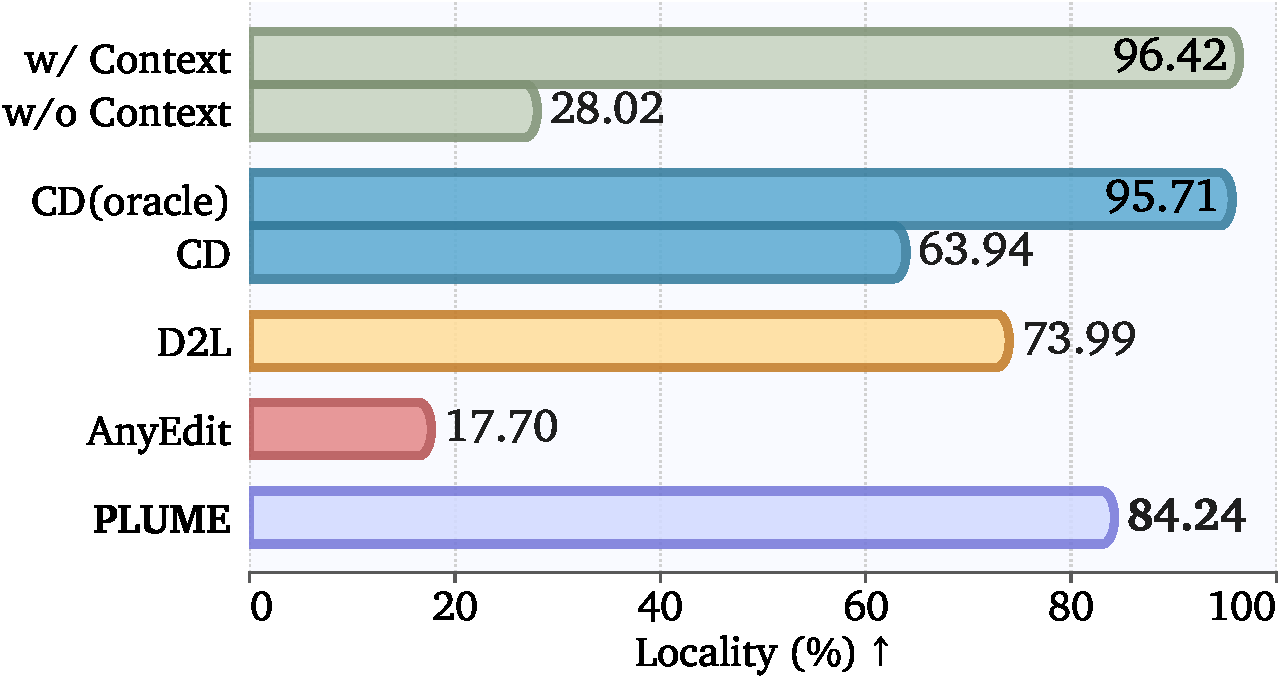
\includegraphics[width=\columnwidth]{fig/results/locality.pdf}
\caption{\textbf{Locality under continual updates.} Higher scores indicate better preservation of information unaffected by context updates.}
\label{fig:locality}
\end{figure}


% 5.4
\subsection{Generalization and Overall Comparison}
\label{sec:generalization_overall}

We extended the continual-update setting to GSM8K and CRUXEval and jointly compared methods across LLM-as-a-Judge, ROUGE-L Recall, Efficiency, and Locality. \method{} consistently outperformed parameterized baselines across both models on mathematical and code reasoning tasks, as shown in Table~\ref{tab:cross_task_generalization}, demonstrating generalization beyond the QA format of \benchmark{}. Its gains were further balanced across multiple dimensions rather than concentrated on a single metric, as illustrated in Figure~\ref{fig:overall_radar}, while preserving strong efficiency and robust information retention across repeated updates under the same evaluation protocol.

% \begin{table}[t]
% \centering
% \footnotesize
% \setlength{\tabcolsep}{3.1pt}
% \renewcommand{\arraystretch}{1.08}
% % Keep the model-band background flush with the horizontal rule above it.
% \setlength{\aboverulesep}{0pt}
% \setlength{\belowrulesep}{0pt}
% \resizebox{\columnwidth}{!}{%
% \begin{tabular}{lrrrr}
% \toprule[1.2pt]
% \multicolumn{1}{c}{\multirow{2}{*}{\textbf{Method}}} & \multicolumn{2}{c}{\textbf{GSM8K}} & \multicolumn{2}{c}{\textbf{CRUXEval}} \\
% \cmidrule(l{0pt}r{1pt}){2-3}\cmidrule(l{1pt}r{0pt}){4-5}
% & \textbf{Recall} & \textbf{LLM} & \textbf{Recall} & \textbf{LLM} \\
% \midrule[1.2pt]
% \multicolumn{5}{c}{\cellcolor{modelshade}\textbf{Qwen3}} \\
% Base w/ context  & 54.21 & 52.76 & 68.43 & 55.37 \\
% Base w/o context & 15.21 &  7.82 & 37.75 &  4.62 \\
% CD (oracle)      & 51.54 & 50.83 & 65.07 & 53.20 \\
% D2L (oracle)     & 36.23 & 30.24 & 44.09 & 20.50 \\
% AnyEdit (AlphaEdit) & 16.99 &  1.90 & 44.41 & 10.50 \\
% CD               & \underline{36.40} & \underline{26.31} & \underline{51.52} & \underline{13.75} \\
% D2L              & 23.18 & 16.42 & 39.48 & 13.63 \\
% \midrule[0.5pt]
% \textbf{PLUME}   & \textbf{45.39} & \textbf{41.47} & \textbf{62.31} & \textbf{50.62} \\
% \midrule[1.2pt]
% \multicolumn{5}{c}{\cellcolor{modelshade}\textbf{Gemma2}} \\
% Base w/ context  & 42.90 & 39.86 & 47.37 & 33.23 \\
% Base w/o context & 10.12 &  4.41 & 18.07 &  2.96 \\
% CD (oracle)      & 41.96 & 39.92 & 47.09 & 31.81 \\
% D2L (oracle)     & 22.23 & 15.29 & 34.36 & 12.83 \\
% AnyEdit (AlphaEdit) & 10.67 &  1.26 & \underline{34.35} &  6.77 \\
% CD               & \underline{23.03} & \underline{12.52} & 30.55 & 10.74 \\
% D2L              & 20.04 & 11.74 & 29.95 & \underline{11.44} \\
% \midrule[0.5pt]
% \textbf{PLUME}   & \textbf{33.69} & \textbf{29.65} & \textbf{40.52} & \textbf{26.12} \\
% \bottomrule[1.2pt]
% \end{tabular}
% }
% \caption{\textbf{Cross-task generalization on GSM8K and CRUXEval.} We reported ROUGE-L Recall and LLM-as-a-Judge scores across Qwen3 and Gemma2.}
% \label{tab:cross_task_generalization}
% \end{table}

\begin{table}[t]
\centering
\footnotesize
\setlength{\tabcolsep}{3.1pt}
\renewcommand{\arraystretch}{1.08}
% Keep the model-band background flush with the horizontal rule above it.
\setlength{\aboverulesep}{0pt}
\setlength{\belowrulesep}{0pt}
\resizebox{\columnwidth}{!}{%
\begin{tabular}{lrrrr}
\toprule[1.2pt]
\multicolumn{1}{c}{\multirow{2}{*}{\textbf{Method}}} & \multicolumn{2}{c}{\textbf{GSM8K}} & \multicolumn{2}{c}{\textbf{CRUXEval}} \\
\cmidrule(l{0pt}r{1pt}){2-3}\cmidrule(l{1pt}r{0pt}){4-5}
& \textbf{Recall} & \textbf{LLM} & \textbf{Recall} & \textbf{LLM} \\
\midrule[1.2pt]
\multicolumn{5}{c}{\cellcolor{modelshade}\textbf{Qwen3}} \\
w/ Context (oracle) & 54.21 & 52.76 & 68.43 & 55.37 \\
CD (oracle)      & 51.54 & 50.83 & 65.07 & 53.20 \\
D2L (oracle)     & 36.23 & 30.24 & 44.09 & 20.50 \\
\midrule
w/o Context       & 15.21 &  7.82 & 37.75 &  4.62 \\
AnyEdit           & 16.99 &  1.90 & 44.41 & 10.50 \\
CD               & \underline{36.40} & \underline{26.31} & \underline{51.52} & \underline{13.75} \\
D2L              & 23.18 & 16.42 & 39.48 & 13.63 \\
\midrule[0.5pt]
\textbf{PLUME}   & \textbf{45.39} & \textbf{41.47} & \textbf{62.31} & \textbf{50.62} \\
\midrule[1.2pt]
\multicolumn{5}{c}{\cellcolor{modelshade}\textbf{Gemma2}} \\
w/ Context (oracle) & 42.90 & 39.86 & 47.37 & 33.23 \\
CD (oracle)      & 41.96 & 39.92 & 47.09 & 31.81 \\
D2L (oracle)     & 22.23 & 15.29 & 34.36 & 12.83 \\
\midrule
w/o Context       & 10.12 &  4.41 & 18.07 &  2.96 \\
AnyEdit           & 10.67 &  1.26 & \underline{34.35} &  6.77 \\
CD               & \underline{23.03} & \underline{12.52} & 30.55 & 10.74 \\
D2L              & 20.04 & 11.74 & 29.95 & \underline{11.44} \\
\midrule[0.5pt]
\textbf{PLUME}   & \textbf{33.69} & \textbf{29.65} & \textbf{40.52} & \textbf{26.12} \\
\bottomrule[1.2pt]
\end{tabular}
}
\caption{\textbf{Cross-task generalization on GSM8K and CRUXEval.} We reported ROUGE-L Recall and LLM-as-a-Judge scores across Qwen3 and Gemma2.}
\label{tab:cross_task_generalization}
\end{table}


\begin{figure}[!t]
\centering
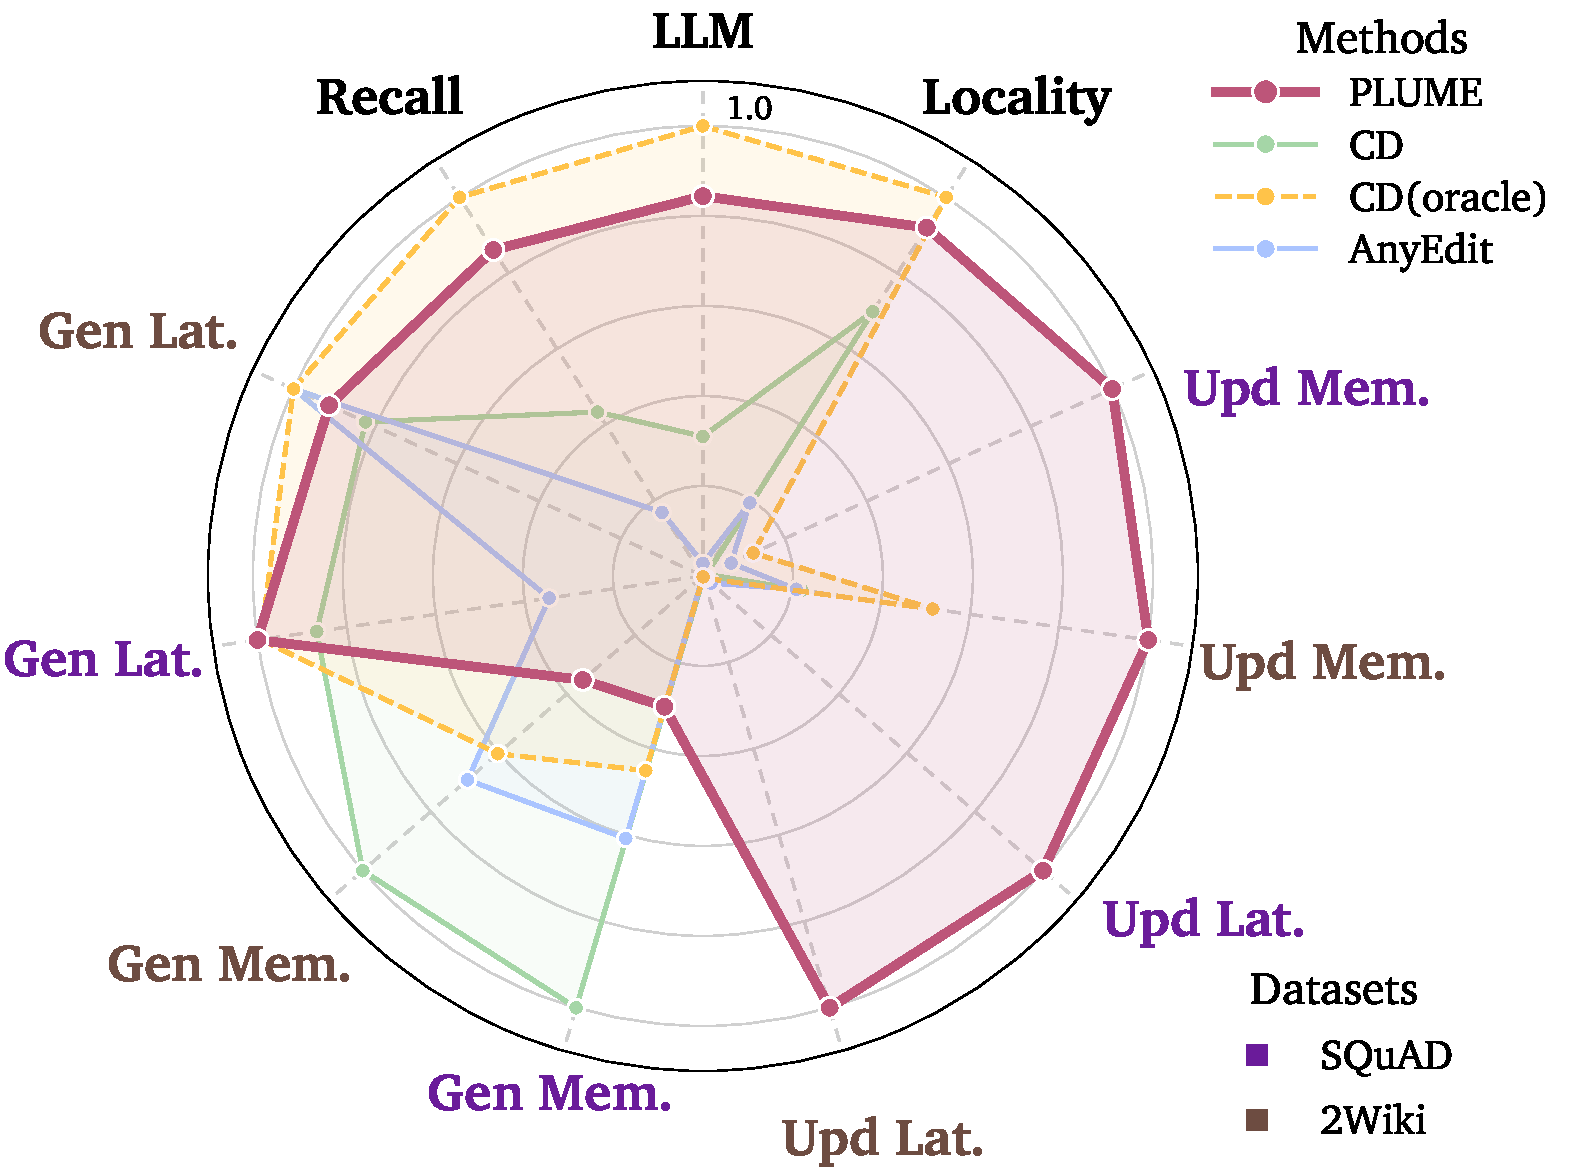
\includegraphics[width=1\columnwidth]{fig/results/radar_chart.pdf}
\caption{\textbf{Overall comparison of effectiveness and efficiency.} Metrics include answer quality, locality, and update/generation efficiency on SQuAD and 2Wiki, normalized such that higher values are better.}
\label{fig:overall_radar}
\end{figure}


% Ablation Figure
\begin{figure}[t]
\centering
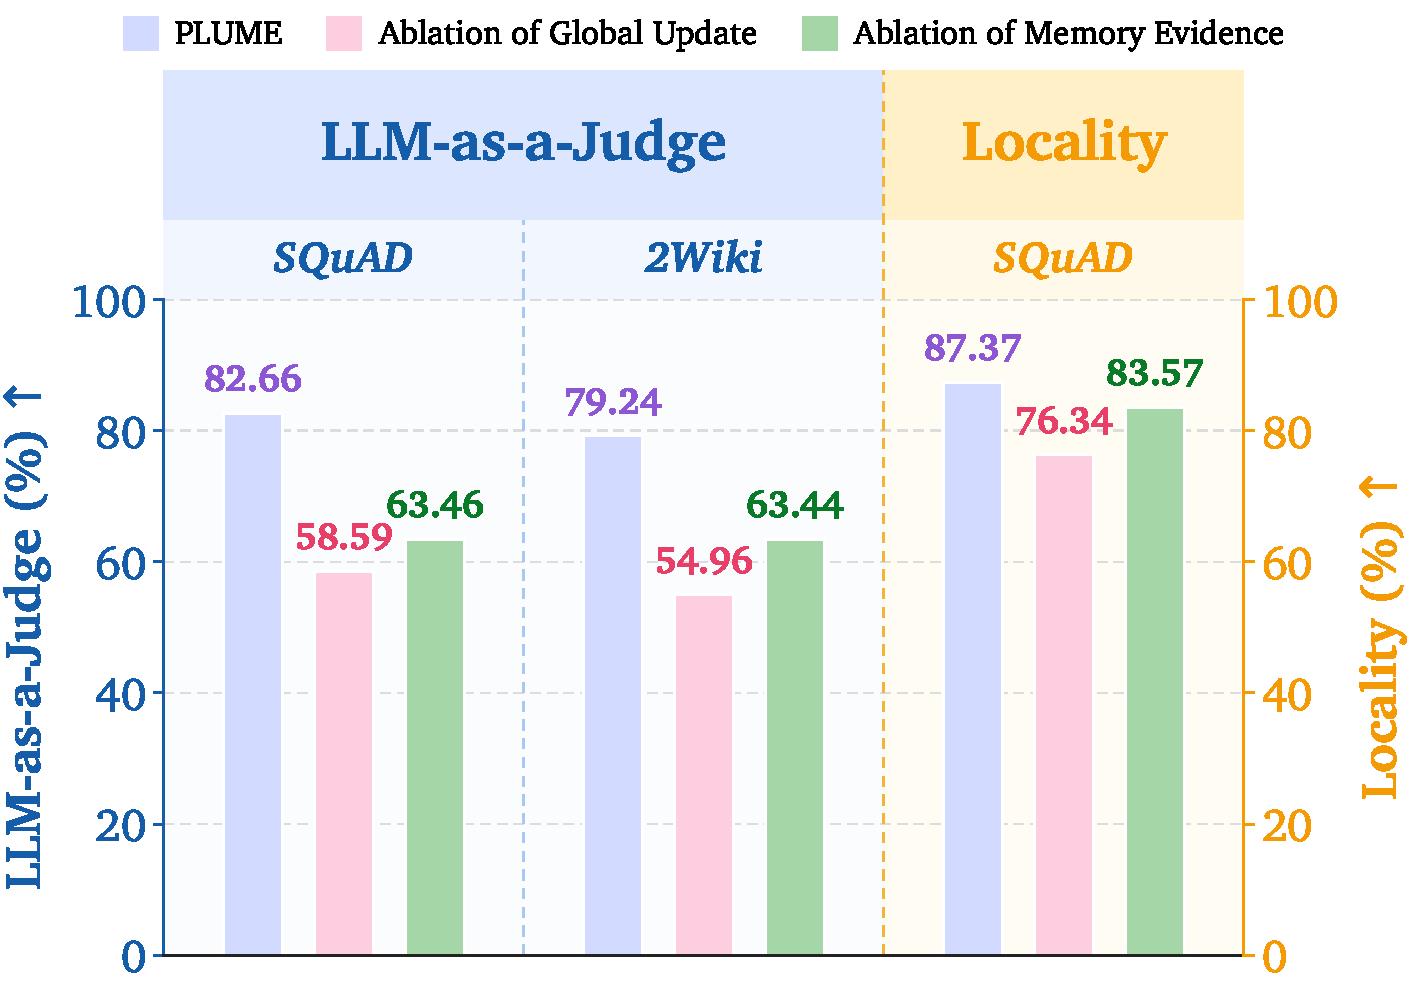
\includegraphics[width=1\columnwidth]{fig/results/ablation_study.pdf}
\caption{\textbf{Ablation of \method{} components.} Removing either the global update representation or memory evidence degrades performance, with the former causing a larger drop.}
\label{fig:ablation}
\end{figure}

% 5.5 Ablation
\subsection{Ablation Study}
\label{sec:ablation}

We ablated two core components of \method{}---the global update representation and query-activated memory evidence---by removing each component individually. Both ablations consistently reduced LLM-as-a-Judge performance on SQuAD and 2Wiki, as well as Locality on SQuAD, as shown in Figure~\ref{fig:ablation}. Removing the global update representation led to substantially larger degradation, underscoring its importance in capturing the current context state, whereas removing memory evidence eliminated the query-specific information that improved answer quality and preserved unaffected knowledge. Together, the two components offered complementary, non-redundant signals essential to \method{}'s overall performance.

% Case Study
\begin{figure*}[t]
    \centering
    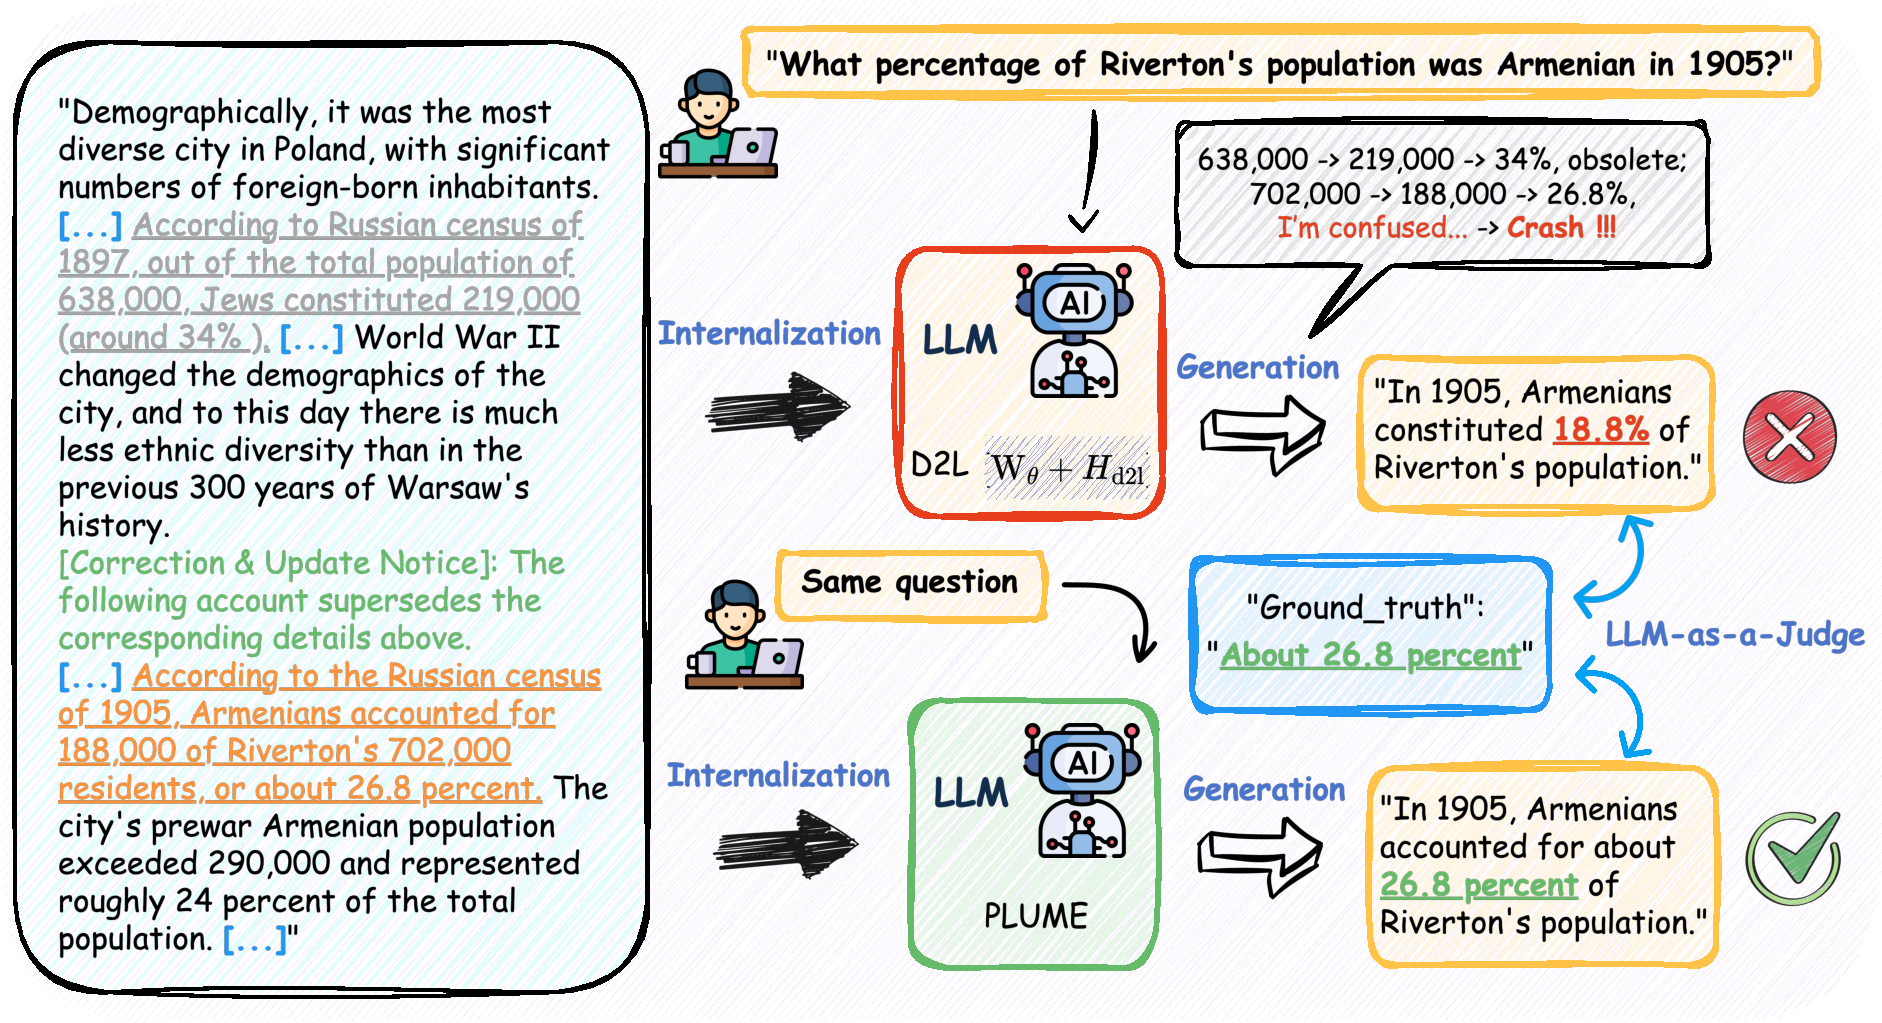
\includegraphics[width=1\textwidth]{fig/case_study/case_study_bg.pdf}
    \caption{\textbf{Representative case under a context update.} D2L conflates information with different validity states and produces an incorrect answer, whereas \method{} follows the currently valid update.}
    \label{fig:case_study}
\end{figure*}

\subsection{Case Study}
\label{sec:case_study}
Representative cases exhibited valid, invalid, and unaffected information coexisting within the same parameterized state, underscoring a considerable disambiguation challenge.
As shown in Figure~\ref{fig:case_study}, D2L failed to distinguish these validity states and produced an incorrect answer, whereas \method{} emphasized the latest update and activated the corresponding memory evidence to follow the currently valid information.
This behavior corroborates the validity-state interference observed in the aggregate results, further supporting our quantitative findings.


\section{Related Work}
\label{sec:related-work}

\paragraph{Context Internalization.}

% RAG~\citep{gao2023retrieval} and long-context models~\citep{ding2023longnet} provide context at inference time, requiring repeated processing. 
% Context parameterization instead internalizes context for reuse across queries.
% CD transfers context-induced behavior into model parameters~\citep{snell2022learning}, while D2L compiles context into lightweight parameterized representations~\citep{charakorn2026doc}.
% However, these methods mainly assume static, internally consistent contexts and do not explicitly handle validity changes under subsequent updates.
RAG~\citep{gao2023retrieval} and long-context models~\citep{ding2023longnet} supply context at inference time, incurring repeated overhead.
Context parameterization instead internalizes context into reusable representations.
CD transfers context-induced behavior into model parameters~\citep{snell2022learning}, while D2L compiles context into lightweight parameterized representations~\citep{charakorn2026doc}.
Both, however, presuppose static, internally consistent contexts, leaving validity changes under updates unaddressed.


\paragraph{Knowledge Editing and Continual Updates.}
Knowledge editing updates factual knowledge in language models without full retraining~\citep{yao2023editing}, exemplified by ROME, MEMIT, and AlphaEdit~\citep{meng2022locating,meng2023massediting,fang2025alphaedit}.
Recent work examined sequential editing, interference, and knowledge preservation~\citep{wang2024knowledge,chen2024lifelong,jiang2024learning,li2025reinforced}.
Our setting instead considers continual updates to parameterized contexts with factual dependencies and unaffected information.


\paragraph{Knowledge Conflicts.}
Prior work mainly studied conflicts between parametric knowledge and external context~\citep{xie2024adaptive,shi2024ircan}, or among retrieved contexts~\citep{cattan2025dragged,xu2024knowledge}.
These settings retained conflicting evidence at inference time.
In contrast, our setting considers currently valid and invalidated information already internalized into parameters, without direct access to the original context.
\benchmark{} and \method{} are designed for this setting.

% % \section{Conclusion}

% % This paper introduces and formalizes the In-Place Instruction Following task and constructs a benchmark spanning three difficulty levels. Through an attention-bias probe, we find evidence that insufficient prioritization of the constraint span is one source of failure in vanilla dLLMs during parallel denoising. To address this, we propose \method, a post-training framework combining \sft and \vrpo. Additionally, a fine-grained evaluation reveals a persistent trade-off between local and global consistency in style constraint scenarios.


% % \section*{Limitations}

% % While \method improves in-place instruction following in dLLMs, this work has several limitations. First, \benchmark{} mainly focuses on text-only in-place instruction following, and its coverage of multilingual, multimodal, and interactive editing scenarios remains limited. Second, although the proposed evaluation protocol combines automatic, reward-model-based, and human judgments, rubric-based evaluation may still be affected by evaluator bias, especially for style and discourse-function constraints. Third, \method is evaluated on four representative dLLMs, but its scalability to larger diffusion models and its robustness under more complex or conflicting anchors require further investigation. Future work may extend IIF to broader domains and develop more interpretable mechanisms for local--global constraint coordination.


% \section{Conclusion}
% \label{sec:conclusion}

% % 本文研究持续更新文档的参数化记忆。现有上下文参数化方法能够将文档编译为可复用参数，但通常假设文档静态且内部一致；当后续修正与原始内容被共同写入时，模型容易混合当前事实与失效事实。因此，可靠的参数化记忆不仅需要高效写入文档，还需要显式建模知识的覆盖关系与查询相关读取。

% % 为此，我们提出 \task{} 任务，并通过 FLUID 在五个问答基准上构建 \benchmark{}，统一评估更新采用、旧知抑制和知识保持。我们进一步提出 \method{}，联合完整文档状态、新旧 LoRA 的更新方向与查询相关记忆证据，并通过自适应解码调用当前有效知识。跨数据集、模型和任务的实验以及消融分析验证了 \method{} 的有效性，为构建可更新、可复用的长期参数记忆提供了新的评测基础与方法路径。


% % This paper studies parametric memory updates for continually evolving context. Existing context parameterization methods can compile context into reusable parameters, thereby avoiding repeated encoding of the full context for every query. However, they typically assume that the context is static and internally consistent. When outdated information and subsequent updates are jointly encoded into the same parameter state, models can easily conflate currently valid facts with obsolete ones. Reliable parametric memory therefore requires not only efficient context parameterization, but also an explicit representation of how new knowledge supersedes old knowledge.

% % To this end, we introduce the \task{} task and construct \benchmark{} from five public question-answering datasets, with LLM-as-a-Judge metrics for evaluating adherence to updated knowledge. We further propose \method{}, which preserves the global context state through a full-history LoRA, amplifies the update direction through the difference between the new and old LoRAs, and adaptively integrates query-relevant memory evidence during decoding. Experiments and ablation studies across datasets and model backbones consistently demonstrate the effectiveness of these designs, establishing a benchmark and method for studying reusable and reliably updatable long-term parametric memory.

% This paper studies context parameterization under continual updates, where contextual information is internalized into reusable parameterized states and subsequently revised as new information arrives. 
% Existing context parameterization methods can efficiently compile context into reusable parameters, avoiding repeated processing of the full context for each query.
% However, they typically assume that the context is static and internally consistent. 
% When previously valid information and subsequent updates are jointly parameterized, models may conflate currently valid knowledge with invalidated information.
% Reliable context parameterization under continual updates therefore requires not only efficient reuse, but also effective incorporation of updates while preserving unaffected knowledge.

% To study this setting, we introduce the \task{} task and construct \benchmark{} from five public question-answering datasets, using LLM-as-a-Judge to evaluate model adherence to currently valid information. 
% We further propose \method{}, which preserves global contextual information through a full-history LoRA, amplifies the update direction using the parameter difference between pre- and post-update LoRAs, and adaptively integrates query-conditioned memory evidence during decoding. 
% Experiments and ablation studies across multiple datasets and model backbones consistently demonstrate the effectiveness of these components, establishing \benchmark{} and \method{} as a benchmark and method for studying reusable and reliably updatable parameterized context.







\section{Conclusion}
\label{sec:conclusion}
This paper studied context parameterization under continual updates. We introduced \task{} and constructed \benchmark{}, comprising five question-answering datasets, to jointly evaluate the fidelity of update integration and the stability of unaffected information. We further proposed \method{}, integrating global update representation with query-activated memory evidence. Experiments and ablations across datasets and backbones confirmed its effectiveness for reliable context parameterization in this setting, extending this paradigm to the dynamically evolving information environments that prior work has largely overlooked.

\flushbottom


% Entries for the entire Anthology, followed by custom entries
% \bibliography{custom, custom_graft}
\bibliography{custom}

\clearpage
\appendix
\section{LLM Usage Statement}
We utilized Large Language Models to assist with the writing and polishing of the manuscript, including improvements to grammar, clarity, conciseness, and word choice. The models were used exclusively as writing aids and did not contribute to the development of the research ideas, methodology, experiments, or scientific conclusions.


\section{Detailed Setup}
\label{app:detailed-setup}
In this section, we provide additional details regarding the models, benchmark, datasets, and baseline methods used in our experiments.


\subsection{Models}
\label{app:models}
We used two base language models and their corresponding pretrained D2L hypernetworks:
\begin{itemize}
    \item \textbf{Qwen3-4B-Instruct-2507.}
    Qwen3-4B-Instruct-2507 is a 4B-parameter instruction-tuned autoregressive language model from the Qwen3 family~\citep{yang2025qwen3}. It served as our primary backbone and provided a relatively strong instruction-following capability at a moderate model scale. We downloaded the \texttt{Qwen/Qwen3-4B-Instruct-2507} checkpoint from Hugging Face.

    \item \textbf{Gemma-2-2B-it.}
    Gemma-2-2B-it is a 2B-parameter instruction-tuned autoregressive language model from the Gemma 2 family~\citep{team2024gemma}. Compared with Qwen3-4B-Instruct-2507, it provided a smaller and architecturally distinct backbone for evaluating the robustness of our method across model families and scales. We downloaded the \texttt{google/gemma-2-2b-it} checkpoint from Hugging Face.

    \item \textbf{Qwen-4B D2L hypernetwork.} The Qwen-4B D2L hypernetwork is a pretrained context-to-parameter model that maps textual context directly into LoRA parameters conditioned on the target backbone, Qwen3-4B-Instruct-2507~\citep{charakorn2026doc}.
    It enables long-form context information to be compressed into a lightweight parametric representation without directly modifying the frozen backbone parameters.
    We used the \texttt{qwen\_4b\_d2l/checkpoint-20000} checkpoint after 20K training steps.

    \item \textbf{Gemma-2B D2L hypernetwork.} The Gemma-2B D2L hypernetwork performs the same context-to-LoRA parameterization for the smaller Gemma-2-2B-it backbone~\citep{charakorn2026doc}.
    Its backbone-specific parameter generation allowed us to evaluate D2L consistently across model families and at a reduced parameter scale.
    We used the \texttt{gemma\_2b\_d2l/checkpoint-20000} checkpoint, matching the identical training budget used for Qwen.
\end{itemize}
Since \method{} is a training-free approach, both the base models and the D2L hypernetworks remained frozen throughout evaluation, without requiring any additional parameter updates.


\subsection{Benchmark and Datasets}
\label{app:benchmark-datasets}

\paragraph{Benchmark.}
As shown in Table~\ref{tab:dataset-statistics}, we provide the detailed statistics of \benchmark{}. The benchmark contains \textbf{2,944 contexts} and \textbf{12,932 question--answer pairs}. Across all five constituent datasets, the context-weighted mean full-history length is \textbf{3,811.9 tokens}, measured using the Qwen3-4B-Instruct-2507 tokenizer. The per-dataset averages range from 328.3 tokens for SQuAD to 18,539.8 tokens for 2WikiMultihopQA, reflecting substantial variation in context length across the benchmark.

\paragraph{Datasets.}
In total, we employed seven datasets spanning factual and reasoning-intensive settings.
The first five constitute \benchmark{}, while GSM8K and CRUXEval were additionally included to assess whether \method{}, together with the compared baseline and oracle methods, generalizes beyond factual QA to more challenging mathematical and code reasoning.
For all datasets, we constructed and annotated samples under our context-update setting, ensuring that every method was evaluated under an identical protocol across domains.

\begin{itemize}

\item \textbf{SQuAD.}
The Stanford Question Answering Dataset (SQuAD)~\citep{rajpurkar2016squad} is an extractive question-answering dataset comprising questions over Wikipedia passages, with answers grounded in textual spans.
We annotated selected samples with context updates and corresponding question--answer labels following our benchmark construction procedure.
We used the \texttt{rajpurkar/squad} dataset from Hugging Face.
A representative annotated example is shown in Figure~\ref{fig:squad-example}.

\item \textbf{ROPES.}
Reasoning Over Paragraph Effects in Situations (ROPES)~\citep{lin2019reasoning} evaluates whether models can apply causal or qualitative relationships described in background passages to reason about novel, unseen situations.
We annotated selected samples by updating answer-relevant information and its associated dependencies while maintaining contextual consistency.
We used the \texttt{allenai/ropes} dataset from Hugging Face.
A representative annotated example is shown in Figure~\ref{fig:ropes-example}.

\item \textbf{2WikiMultihopQA.}
2WikiMultihopQA~\citep{ho2020constructing} is a multi-hop question-answering dataset that requires compositional reasoning over multiple supporting facts from Wikipedia passages.
We annotated selected samples by modifying answer-supporting facts and consistently updating information involved in the corresponding reasoning dependencies.
We used the \texttt{xanhho/2WikiMultihopQA} dataset from Hugging Face.
A representative annotated example is shown in Figure~\ref{fig:2wiki-example}.

\item \textbf{MultiFieldQA-en.}
MultiFieldQA-en is a single-document question-answering dataset from LongBench~\citep{bai2024longbench}, containing long-form contexts collected from diverse domains and disciplines.
We annotated selected samples with context updates while preserving the remaining information and structure of the original long context.
We used the \texttt{multifieldqa\_en} subset of \texttt{THUDM\/LongBench} from Hugging Face.
A representative annotated example is shown in Figure~\ref{fig:longbench-example}.

\item \textbf{QASPER.}
QASPER~\citep{dasigi2021dataset} is a question-answering dataset built upon scientific papers, where answering a question may require synthesizing evidence distributed across multiple sections.
We annotated selected samples by updating answer-relevant evidence and its dependent information while preserving the overall structure and coherence of the original context.
We used the \texttt{allenai/qasper} dataset from Hugging Face.
A representative annotated example is shown in Figure~\ref{fig:qasper-example}.

\item \textbf{GSM8K.}
Grade School Math 8K (GSM8K)~\citep{cobbe2021training} contains linguistically diverse grade-school mathematical word problems that typically require multi-step arithmetic reasoning to solve correctly.
We annotated selected samples under our context-update setting to evaluate whether the same update mechanism generalized beyond question answering to mathematical reasoning.
We used the \texttt{openai/gsm8k} dataset from Hugging Face.

\item \textbf{CRUXEval.}
CRUXEval~\citep{gu2024cruxeval} is a code reasoning benchmark consisting of short Python functions paired with input--output examples, covering both input and output prediction tasks.
We annotated selected samples under our context-update setting to evaluate generalization to structured code reasoning.
We used the \texttt{cruxeval-org/cruxeval} dataset from Hugging Face.

\end{itemize}

\begin{figure}[t]
    \centering
    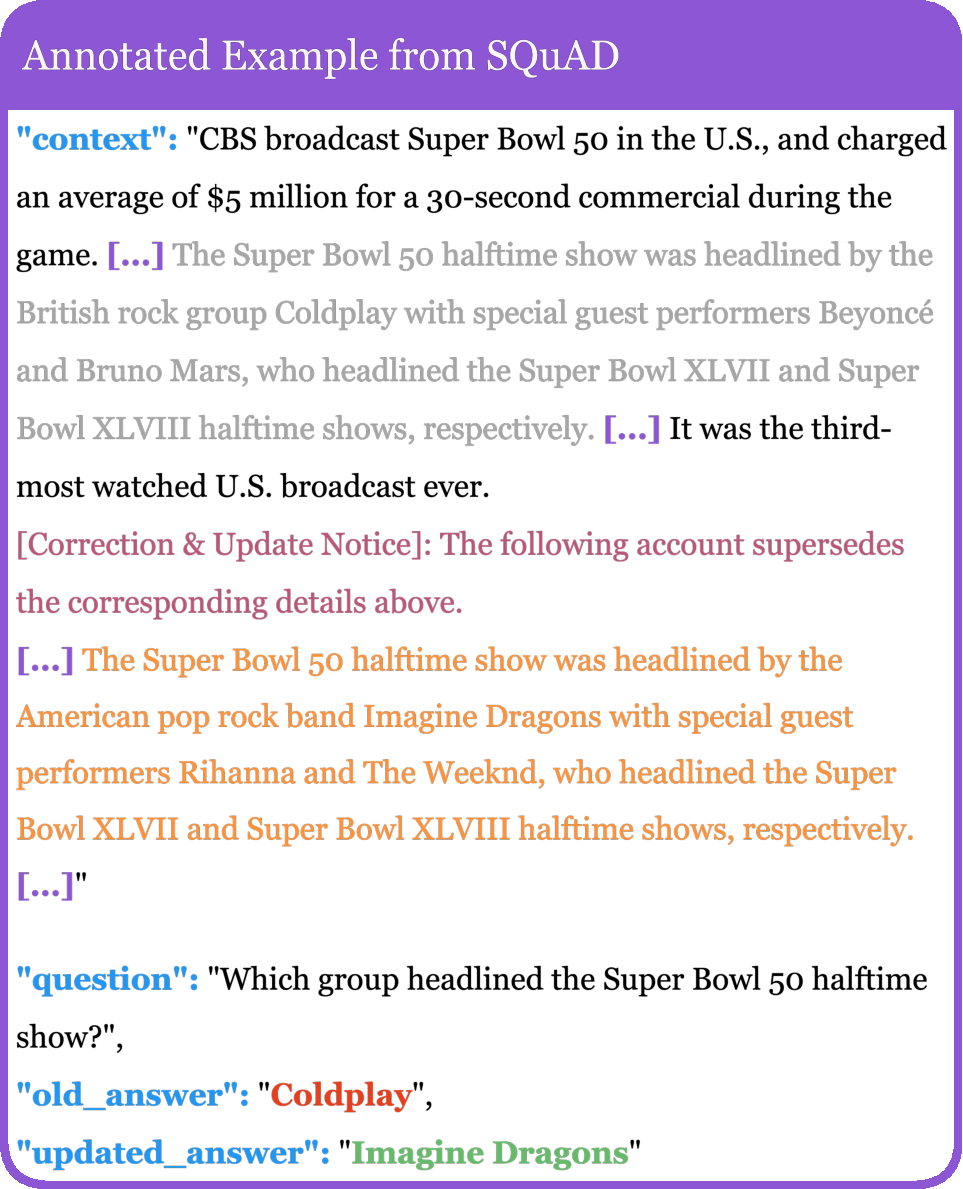
\includegraphics[width=\columnwidth]{fig/dataset/1-squad.pdf}
    \caption{\textbf{Representative \benchmark{} example derived from SQuAD.} The example illustrates the original context, its subsequent update, and the associated question--answer annotations.}
    \label{fig:squad-example}
\end{figure}

\begin{figure}[t]
    \centering
    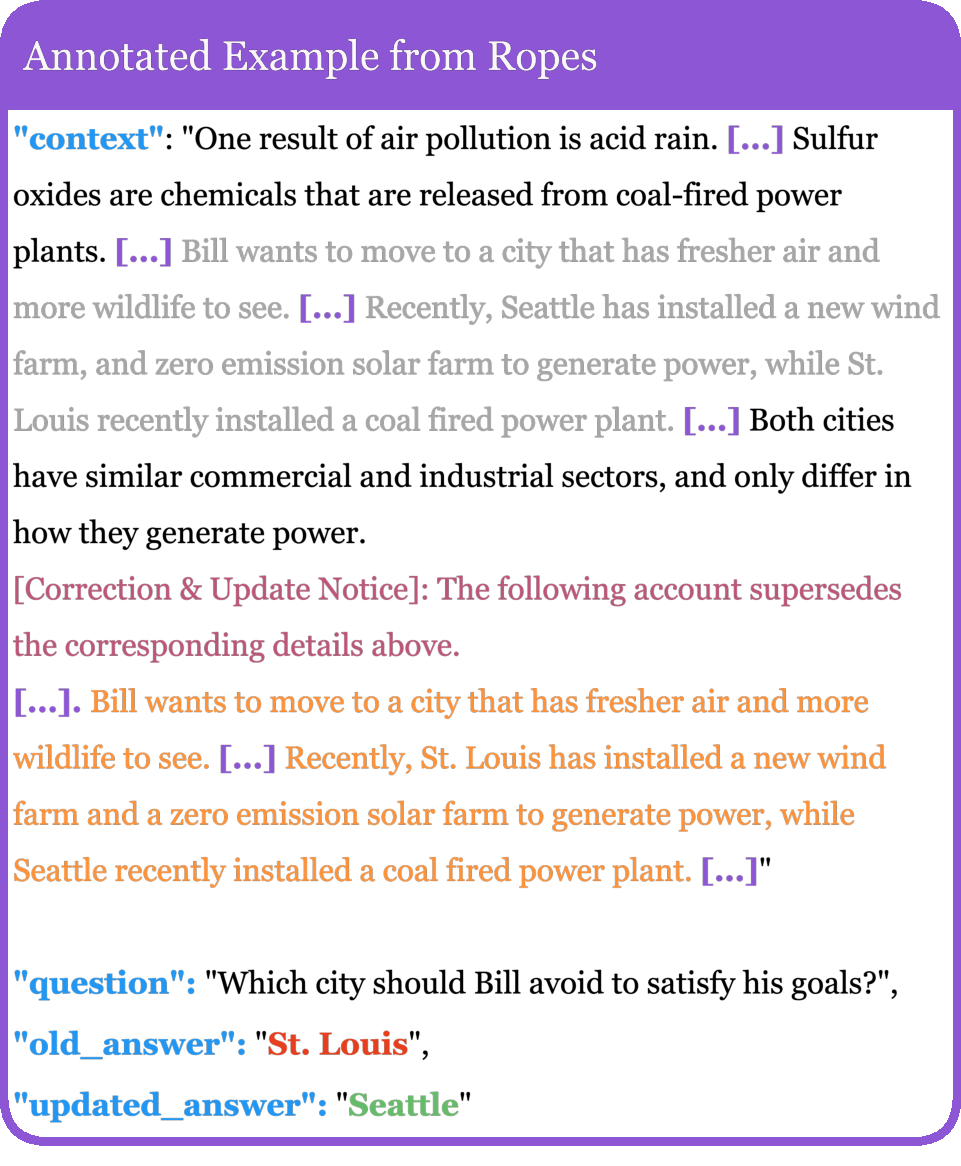
\includegraphics[width=\columnwidth]{fig/dataset/2-ropes.pdf}
    \caption{\textbf{Representative \benchmark{} example derived from ROPES.} The example illustrates a context update while preserving the causal reasoning structure of the original instance.}
    \label{fig:ropes-example}
\end{figure}

\begin{figure}[t]
    \centering
    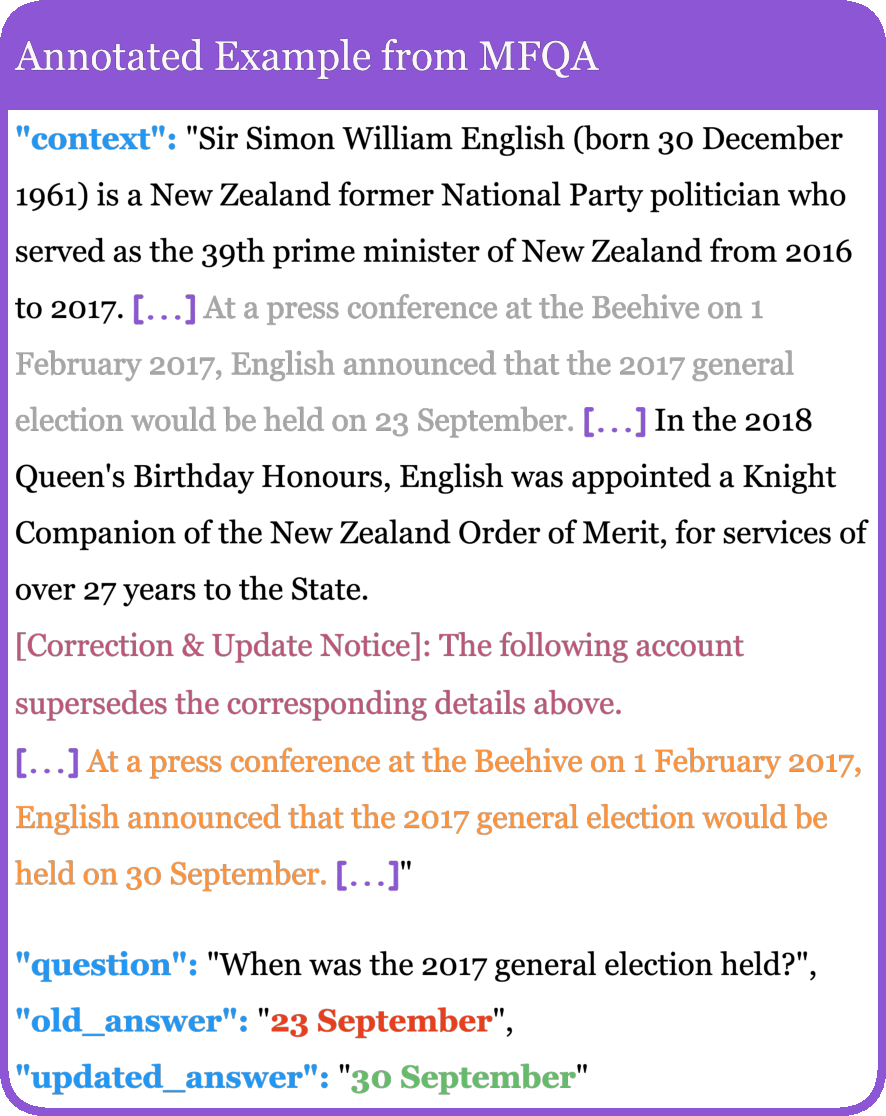
\includegraphics[width=\columnwidth]{fig/dataset/3-mfqa.pdf}
    \caption{\textbf{Representative \benchmark{} example derived from MultiFieldQA-en.} The example illustrates an update within a long-form context while retaining its original document structure.}
    \label{fig:longbench-example}
\end{figure}

\begin{figure}[t]
    \centering
    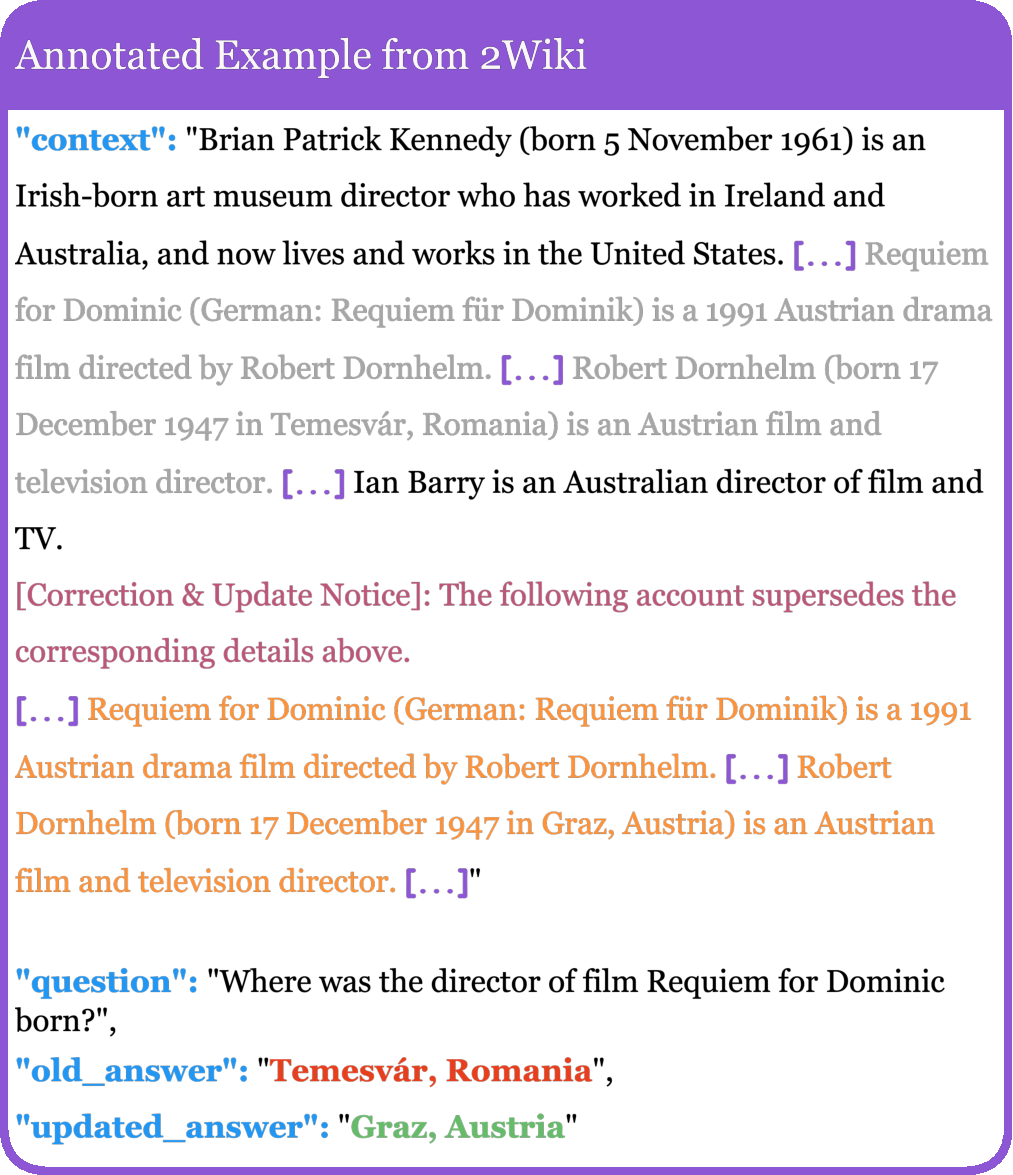
\includegraphics[width=\columnwidth]{fig/dataset/4-2wiki.pdf}
    \caption{\textbf{Representative \benchmark{} example derived from 2WikiMultihopQA.} The example illustrates a context update with consistently revised multi-hop dependencies.}
    \label{fig:2wiki-example}
\end{figure}

\begin{figure}[t]
    \centering
    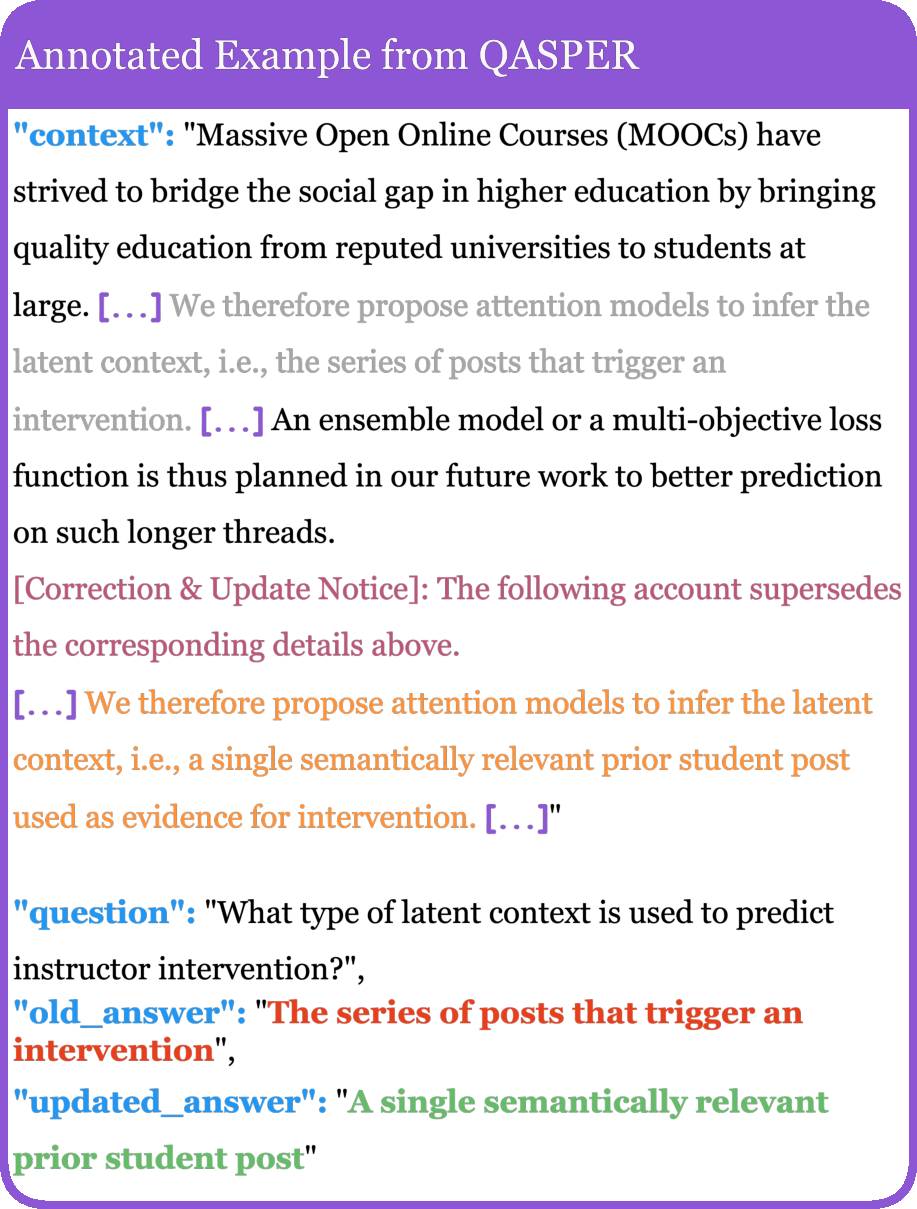
\includegraphics[width=\columnwidth]{fig/dataset/5-qasper.pdf}
    \caption{\textbf{Representative \benchmark{} example derived from QASPER.} The example illustrates an update to evidence distributed across a scientific document.}
    \label{fig:qasper-example}
\end{figure}

Table~\ref{tab:dataset-statistics} reports the number of contexts, the number of question--answer pairs, and the average full-context length for the five datasets constituting \benchmark{}. Context length is measured using the Qwen3-4B-Instruct-2507 tokenizer.


\begin{table}[tb]
\centering
\small
\resizebox{\columnwidth}{!}{%
\begin{tabular}{lrrr}
\toprule
\textbf{Dataset} & \textbf{Contexts} & \textbf{QA pairs} & \textbf{Avg. context tokens} \\
\midrule
SQuAD             & 2,067 & 10,570 & 328.3 \\
ROPES             &   203 &  1,688 & 434.6 \\
2WikiMultihopQA   &   300 &    300 & 18,539.8 \\
MultiFieldQA-en   &   150 &    150 & 14,068.8 \\
QASPER            &   224 &    224 & 12,424.7 \\
\midrule
\benchmark{}        & 2,944 & 12,932 & 3,811.9 \\
\midrule
GSM8K             & 1,319 &  1,319 & 123.0 \\
CRUXEval          &   800 &    800 & 86.3 \\
\bottomrule
\end{tabular}%
}
\caption{\textbf{Dataset statistics for \benchmark{} and the cross-task evaluation sets.} We report the numbers of contexts and question--answer pairs and the mean full-history length measured with the Qwen3-4B-Instruct-2507 tokenizer.}
\label{tab:dataset-statistics}
\end{table}

\subsection{Baselines}
\label{app:baselines}

We compared \method{} with the following baselines:

\begin{itemize}

\item \textbf{Base Model w/o Context.}
The base model receives only the query and generates the response without access to any contextual information. This setting measures the model's parametric knowledge and serves as a lower-bound reference for context-dependent tasks.

\item \textbf{Base Model w/ Context (oracle).}
The base model receives the complete context history together with the query at inference time. Unlike parameterized methods, it directly accesses the textual context during generation and therefore serves as a full-context reference.

\item \textbf{D2L.}
Doc-to-LoRA (D2L)~\citep{charakorn2026doc} parameterizes textual context into LoRA adapters using a pretrained hypernetwork. We used the official pretrained hypernetwork checkpoint corresponding to each backbone. For contexts longer than the supported input length, we divided the full context history into chunks of at most 8,192 tokens and followed the original iterative layer-wise adapter generation procedure. The generated rank-8 LoRA adapters were applied to the MLP down-projection layer of each Transformer block.
The hypernetwork is trained across contexts with the same teacher--student
principle as context distillation: a context-conditioned teacher supplies the
target behavior, while the generated adapter enables the student to reproduce
that behavior without receiving the context at query time. Architecturally,
D2L aggregates variable-length context representations with a
Perceiver-style module and uses layer-specific output heads to generate the
LoRA factors. This amortizes the per-context optimization required by CD into
a single hypernetwork pass for a previously unseen context.

\item \textbf{Context Distillation (CD).}
Context Distillation (CD)~\citep{snell2022learning} transfers information from a context-conditioned teacher into model parameters through supervised distillation. For each context, we generated 20 auxiliary question--answer pairs in four rounds of five pairs and used them as distillation examples. We optimized a newly initialized rank-8 LoRA adapter with LoRA alpha 16 for 300 epochs using a learning rate of $10^{-4}$.

\item \textbf{Other oracle references.}
CD (oracle) uses the target evaluation query as its sole distillation query and the response generated by the full-context teacher as its target. A fresh query-specific rank-8 adapter is optimized for 300 iterations with the same LoRA alpha and learning rate as CD, and is then evaluated on that same query without textual context. D2L (oracle) parameterizes only the gold supporting context associated with the target query rather than the complete accumulated history. Both settings use query-specific information unavailable to the non-oracle methods and are therefore upper-bound references, not directly comparable deployment settings.

\item \textbf{AnyEdit.}
AnyEdit~\citep{jiang2025anyedit} is a knowledge-editing baseline that directly modifies model parameters to incorporate updated information. We used its AlphaEdit-ARE configuration. Edits were applied to the MLP down-projection layers of Transformer blocks 4--8. We divided the full context history into chunks of at most 8,192 tokens and used an edit-window size of 50 without overlap, 25 gradient steps per edit window, a learning rate of $0.5$, a weight decay of $0.001$, a clamp-norm factor of $4$, and an $L_2$ coefficient of $10$.

\end{itemize}

Except for Base Model w/ Context (oracle), all parameterized methods answered queries without receiving the full textual context again at inference time. Unless otherwise specified, all methods used the same base model and generation configuration.

\subsection{Evaluation}
\label{app:evaluation-setup}

Following Section~\ref{sec:benchmark-evaluation}, we evaluated answer coverage, semantic correctness, final-answer agreement, and locality. All answer-quality metrics were first computed for individual queries and then averaged within each dataset. When reporting an overall result across datasets, we used the macro-average of the corresponding per-dataset scores so that datasets with more question--answer pairs did not dominate the comparison.

\paragraph{ROUGE-L Overlap Metrics.}
For each query $i$, let $r_i=(r_{i,1},\ldots,r_{i,m_i})$ be the tokenized reference answer, and let $\hat{y}_i=(\hat{y}_{i,1},\ldots,\hat{y}_{i,n_i})$ be the tokenized model output. Denote the length of their longest common subsequence by
\begin{equation}
L_i=\operatorname{LCS}(r_i,\hat{y}_i).
\label{eq:rougel-lcs}
\end{equation}
ROUGE-L Recall measures how much of the reference answer is covered by the model output, whereas ROUGE-L Precision measures how much of the model output is supported by the reference answer:
\begin{equation}
R_i^{\mathrm{L}}=\frac{L_i}{m_i},
\qquad
P_i^{\mathrm{L}}=\frac{L_i}{n_i}.
\label{eq:rougel-recall-precision}
\end{equation}
Their harmonic mean gives ROUGE-L F1:
\begin{equation}
F_{1,i}^{\mathrm{L}}
=
\frac{2P_i^{\mathrm{L}}R_i^{\mathrm{L}}}
{P_i^{\mathrm{L}}+R_i^{\mathrm{L}}},
\label{eq:rougel-f1}
\end{equation}
where the score is defined as zero when the denominator is zero. We computed all three metrics with the \texttt{rouge-score} implementation and enabled stemming. Because the longest common subsequence preserves token order without requiring matched tokens to be contiguous, these metrics accommodate short intervening phrases while still rewarding structurally consistent answer overlap. Our primary lexical metric is ROUGE-L Recall because reference answers are generally concise and answer coverage is more important than matching the reference length or wording exactly. ROUGE-L Precision additionally penalizes unrelated or unnecessarily long generations, while ROUGE-L F1 summarizes the balance between coverage and conciseness. These complementary variants allow us to distinguish omission of reference content from the inclusion of extraneous material. For a dataset $d$ containing query set $\mathcal{Q}_d$, each metric $M\in\{R^{\mathrm{L}},P^{\mathrm{L}},F_1^{\mathrm{L}}\}$ is aggregated as
\begin{equation}
M_d=\frac{1}{|\mathcal{Q}_d|}\sum_{i\in\mathcal{Q}_d}M_i.
\label{eq:rougel-dataset-aggregation}
\end{equation}

\paragraph{Locality.}
Locality measures whether incorporating an update damages information that should remain unchanged. For dataset $d$, let $\mathcal{U}_d\subseteq\mathcal{Q}_d$ denote the queries whose correct answers are unaffected by the update. Because their original and current reference answers are identical, any reduction in answer coverage after context parameterization indicates interference with unaffected information. We computed Locality as the mean ROUGE-L Recall on this unaffected-query subset:
\begin{equation}
\operatorname{Locality}_d
=
\frac{1}{|\mathcal{U}_d|}
\sum_{i\in\mathcal{U}_d}
R_i^{\mathrm{L}}.
\label{eq:locality}
\end{equation}
Update-affected queries are excluded from $\mathcal{U}_d$. Our locality evaluation uses 50 annotated SQuAD contexts containing 754 queries in total. Exactly one answer is changed in each context, leaving 704 unaffected queries for computing Eq.~\ref{eq:locality}. Thus, a higher Locality score means that the method more faithfully preserves answers supported by facts that were not modified, while a lower score indicates collateral interference introduced by context parameterization, parameter editing, or decoding. Locality is reported on a $0$--$100$ scale in the figures.

For D2 Semantic Equivalence and D3 Final-Answer Agreement, we used GPT-5.6-Sol under unified evaluation prompts and criteria. For efficiency, we separately measured latency and peak GPU memory during context parameterization and query generation, as detailed in Appendix~\ref{app:efficiency-measurement}.


\paragraph{Evaluation Rubric.}
\label{app:evaluation-rubric}

We used GPT-5.6-Sol to evaluate each generated answer under two independent rubrics corresponding to D2 Semantic Equivalence and D3 Final-Answer Agreement. Each evaluation instance contained the query, the current reference answer determined by the full context history, and the model output. The judge did not receive $C_{\mathrm{old}}$, $C_{\mathrm{update}}$, or $C_{\mathrm{full}}$. We used a temperature of 0, allowed at most 300 output tokens, and required a JSON object. Each rubric was evaluated in a separate call. The complete evaluation prompts are provided in Appendix~\ref{app:prompts}.

\paragraph{Judgment Output and Aggregation.}
\label{app:rubric-aggregation}

The two rubrics were evaluated independently. For each rubric, the judge returned a binary \texttt{yes}/\texttt{no} decision, a confidence value between 0 and 1, and a brief rationale. A query received an overall LLM-as-a-Judge score of 1 only when both D2 Semantic Equivalence and D3 Final-Answer Agreement were satisfied; otherwise, it received 0. We reported the mean binary score across queries within each dataset.

\subsection{Implementation Details}
\label{app:implementation-details}

All experiments were conducted on two NVIDIA A800 GPUs using bfloat16 precision.


\section{Hyperparameters}
\label{app:hyperparameters}

We separated the backbone and checkpoint configuration, the context-parameterization execution mode, and the \method{}-specific inference hyperparameters. We reported inference settings only; the training configuration of the released D2L hypernetworks was not included. All models and hypernetworks remained frozen and were loaded in bfloat16 precision. Table~\ref{tab:model-d2l-settings} summarizes the backbone and D2L checkpoint configurations.

\begin{table}[tb]
\centering
\small
\renewcommand{\arraystretch}{1.18}
\setlength{\tabcolsep}{4pt}
\begin{tabular}{llll}
\toprule
\textbf{Base model} & \textbf{D2L checkpoint} & \textbf{Rank} & \textbf{Target} \\
\midrule
Qwen3-4B & Qwen D2L-20k & 8 & MLP down \\
Gemma-2-2B & Gemma D2L-20k & 8 & MLP down \\
\bottomrule
\end{tabular}
\caption{\textbf{Backbone and D2L checkpoint configurations.} All models use bfloat16 precision, and the generated rank-8 LoRA adapters are applied to the MLP down-projection layers.}
\label{tab:model-d2l-settings}
\end{table}

\paragraph{Context parameterization.}
For contexts exceeding the supported input length, we preserved the complete context history by dividing it into near-equal contiguous chunks of at most 8,192 tokens. We used two D2L inference modes, summarized in Table~\ref{tab:d2l-inference-modes}. In \textbf{Iterative} mode, the official layer-wise procedure processed the Transformer-layer representations sequentially. In \textbf{Batched} mode, the layer dimension was folded into the batch dimension and the corresponding representations were processed jointly. This execution-mode choice was independent of context chunking: both modes used the same complete-context chunks and generated rank-8 LoRA adapters with the same structure. For \method{}, the query was used only to activate memory evidence and was never passed to the D2L hypernetwork.

\begin{table}[tb]
\centering
\small
\resizebox{\columnwidth}{!}{%
\begin{tabular}{lcc}
\toprule
\textbf{Setting} & \textbf{Iterative} & \textbf{Batched} \\
\midrule
Context coverage & Complete history & Complete history \\
Maximum chunk length & 8,192 & 8,192 \\
Chunk construction & Near-equal, contiguous & Near-equal, contiguous \\
Layer execution & Sequential & Joint batched pass \\
LoRA rank & 8 & 8 \\
Target module & \texttt{down\_proj} & \texttt{down\_proj} \\
Hypernetwork input & Context/evidence only & Context/evidence only \\
\bottomrule
\end{tabular}%
}
\caption{\textbf{D2L inference modes for context parameterization.} Iterative and batched execution differ only in how Transformer-layer representations are processed; both retain complete-context chunking and use the same adapter configuration.}
\label{tab:d2l-inference-modes}
\end{table}

\paragraph{\method{} and generation settings.}
Table~\ref{tab:plume-implementation-settings} summarizes the method-specific and generation hyperparameters.
\method{} separately parameterizes $C_{\mathrm{old}}$ and $C_{\mathrm{full}}$ and constructs the global update LoRA with $\alpha=1$ and $\beta=1$ in Eq.~\ref{eq:global_adapter}. Memory units are formed independently of the 8,192-token full-context chunks while preserving sentence and paragraph boundaries whenever possible. \methodlexical{} activates the highest-scoring unit using lexical relevance. \methodhybrid{} combines lexical and embedding relevance with an embedding-score weight of $0.25$, activates the top three units, restores their original temporal order, and jointly parameterizes them as the local evidence. Both variants used $\lambda_{\max}=2$ and $\tau=0.1$ for adaptive memory evidence decoding. We used greedy decoding with a temperature of 0 and generated at most 256 new tokens for both backbones and all comparison methods.

For lexical routing, text is lowercased and tokenized with the regular expression \texttt{[a-z0-9]+}. Let $Q$ be the set of query terms, $c_{i,t}$ the count of term $t$ in memory unit $m_i$, and $w_t$ its document-level inverse-frequency weight. With $k_1=1.5$ and $W=\sum_{t\in Q}w_t$, the lexical score is
\begin{equation}
\begin{aligned}
s_{\mathrm{lex}}(q,m_i)
&=\frac{1}{2}\frac{\sum_{t:c_{i,t}>0}w_t}{W}
  +\frac{1}{2}\frac{F_i}{F_i+W}, \\
F_i
&=\sum_{t:c_{i,t}>0}w_t
  \frac{c_{i,t}(k_1+1)}{c_{i,t}+k_1}.
\end{aligned}
\label{eq:lexical-router}
\end{equation}
The score is zero for an empty query-term set. \methodhybrid{} linearly combines this score with cosine similarity after mapping the latter to $[0,1]$. Ties are resolved in favor of the latest memory unit, matching the chronological supersession semantics.

\begin{table}[t]
\centering
\small
\resizebox{\columnwidth}{!}{%
\begin{tabular}{lcc}
\toprule
\textbf{Setting} & \textbf{\methodlexical{}} & \textbf{\methodhybrid{}} \\
\midrule
Maximum context-chunk length & 8,192 & 8,192 \\
Evidence activation & Lexical & Lexical + embedding \\
Number of activated units & 1 & 3 \\
Embedding-score weight & -- & 0.25 \\
$\alpha$ / $\beta$ & 1 / 1 & 1 / 1 \\
$\lambda_{\max}$ / $\tau$ & 2 / 0.1 & 2 / 0.1 \\
Maximum new tokens & 256 & 256 \\
Temperature & 0 & 0 \\
Decoding & Greedy & Greedy \\
\bottomrule
\end{tabular}%
}
\caption{\textbf{\method{}-specific and generation hyperparameters.} Memory units are constructed from context structure, so their number varies with the length and organization of each context.}
\label{tab:plume-implementation-settings}
\end{table}


\section{More Experiments}
\label{app:more-experiments}

This section presents supplementary discussion of the main results together
with analyses of \method{}'s hyperparameter sensitivity and computational
efficiency.

\subsection{Additional Analysis of the Main Results}
\label{app:additional-result-analysis}

\paragraph{Continual-update performance.}
Base Model w/ Context (oracle) provides a strong reference because it can directly
access the full context history for every query, but this requires repeatedly
encoding an increasingly long history. In contrast, the parameterized
baselines answer without the textual history and must recover the currently
valid state from a compact parameter representation. Their degradation under
continual updates therefore indicates interference between valid, invalidated,
and unaffected information rather than merely a failure to retrieve a visible
passage. \method{} improves this setting by explicitly modeling the global update
state and supplementing it with query-relevant memory evidence.

\paragraph{Cross-task generalization.}
GSM8K and CRUXEval differ from the five \benchmark{} QA datasets in both output
structure and reasoning process: the former requires multi-step arithmetic,
whereas the latter requires deterministic program reasoning. \method{}'s gains on
both tasks and both backbones show that its benefit is not restricted to a
particular extractive or document-QA format, but extends to broader continual
context-update scenarios.

\paragraph{Overall comparison and component roles.}
The overall comparison jointly considers ROUGE-L Recall, LLM-as-a-Judge,
memory efficiency, inference throughput, and Locality. \method{}'s advantage is
distributed across these dimensions rather than being driven by a single
answer-quality metric. The component analysis further clarifies the division
of labor: the global update representation preserves the full context state
while emphasizing the latest change, and query-activated memory evidence
provides a local parameter view that reduces interference from information
irrelevant to the current query. Their combination accounts for the stronger
balance between update adoption and preservation of unaffected knowledge.

\subsection{Sensitivity to $\lambda_{\max}$}
\label{app:lambda-sensitivity}

We studied the sensitivity of \method{} to $\lambda_{\max}$, which controls the maximum contribution of query-relevant local memory evidence during adaptive decoding. Figure~\ref{fig:lambda-sensitivity} reports ROUGE-L Recall and Locality under different values of $\lambda_{\max}$.

\begin{figure}[t]
\centering
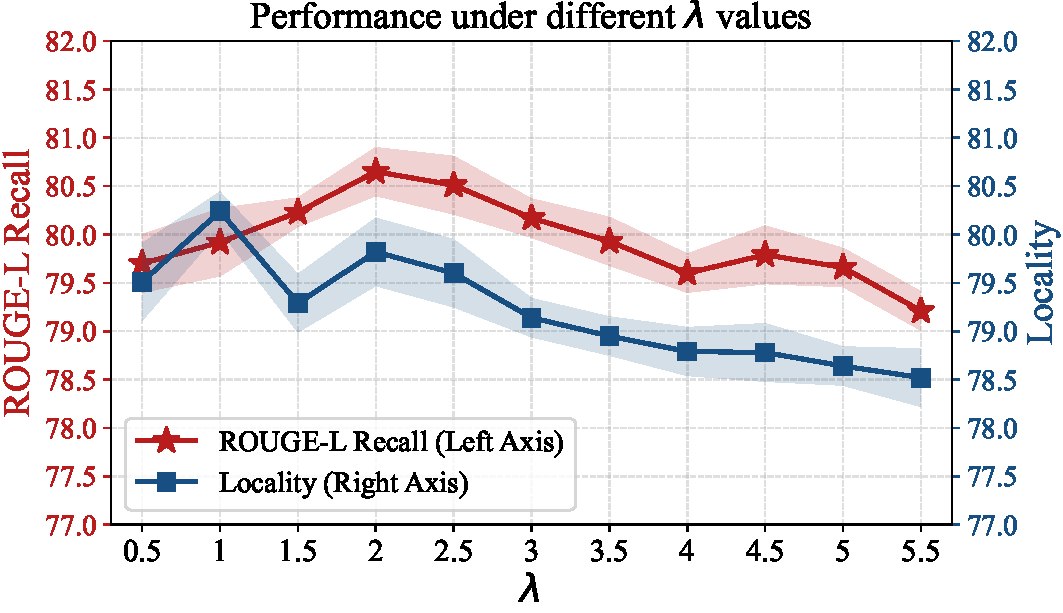
\includegraphics[width=\columnwidth]{fig/results/lambda.pdf}
\caption{\textbf{Sensitivity to the maximum evidence weight $\lambda_{\max}$.} ROUGE-L Recall and Locality remain stable over a broad range, with the strongest overall balance near $\lambda_{\max}=2$; shaded regions indicate variation across runs.}
\label{fig:lambda-sensitivity}
\end{figure}

\method{} remained stable across a broad range of $\lambda_{\max}$ values. Performance was strongest around $\lambda_{\max}=2$, which provided a favorable balance between using query-relevant local evidence and preserving the global context state. Larger values gradually reduced both ROUGE-L Recall and Locality, suggesting that excessive reliance on local evidence could weaken answer quality and information retention. We therefore used $\lambda_{\max}=2$ in the main experiments.

\begin{table*}[!t]
\centering
\small
\setlength{\tabcolsep}{5pt}
\renewcommand{\arraystretch}{1.15}
\providecommand{\MethodHeaderVShift}{-0.3ex}
\begin{tabular}{ccccc}
\toprule
\multirow{2}{*}{\raisebox{\MethodHeaderVShift}{\textbf{Method}}}
& \multicolumn{2}{c}{SQuAD}
& \multicolumn{2}{c}{2Wiki} \\
\cmidrule(lr){2-3}\cmidrule(lr){4-5}
& Mem. (GiB) $\downarrow$
& Lat. (s/document) $\downarrow$
& Mem. (GiB) $\downarrow$
& Lat. (s/document) $\downarrow$ \\
\midrule
CD (oracle)      & 3.568 & 56.600 & 22.376 & 950.085 \\
\midrule
AnyEdit          & \underline{6.332} & 18.754 & 55.028 & 4099.473 \\
CD               & 48.708 & 451.827 & \underline{51.956} & 489.059 \\
D2L              & \textbf{0.438} & \underline{0.466} & \textbf{11.536} & \underline{1.841} \\
\midrule
\textbf{PLUME}   & \textbf{0.438} & \textbf{0.447} & \textbf{11.536} & \textbf{1.832} \\
\bottomrule
\end{tabular}
\caption{
Update efficiency on SQuAD and 2Wiki.
Memory denotes peak update memory, and latency denotes update time per
document. The two base methods are omitted because they incur no update-stage
cost. Excluding the oracle method, bold and underlined values denote the best
and second-best results, respectively. Lower values are better; tied best
values are both bolded.
}
\label{tab:update-efficiency}
\end{table*}

\begin{table*}[!t]
\centering
\small
\setlength{\tabcolsep}{5pt}
\renewcommand{\arraystretch}{1.15}
\providecommand{\MethodHeaderVShift}{-0.3ex}
\begin{tabular}{ccccc}
\toprule
\multirow{2}{*}{\raisebox{\MethodHeaderVShift}{\textbf{Method}}}
& \multicolumn{2}{c}{SQuAD}
& \multicolumn{2}{c}{2Wiki} \\
\cmidrule(lr){2-3}\cmidrule(lr){4-5}
& Mem. (GiB) $\downarrow$
& Lat. (s/query) $\downarrow$
& Mem. (GiB) $\downarrow$
& Lat. (s/query) $\downarrow$ \\
\midrule
Base w/ Context  & 0.208 & 1.972 & 1.749 & 1.194 \\
Base w/o Context & 0.047 & 6.467 & 0.042 & 0.924 \\
CD (oracle)      & 0.057 & 1.663 & 0.053 & 4.709 \\
\midrule
AnyEdit          & 0.042 & 4.789 & 0.046 & \textbf{4.709} \\
CD               & \textbf{0.026} & 1.906 & \textbf{0.032} & 5.718 \\
D2L              & \underline{0.039} & \textbf{1.577} & \underline{0.045} & 5.079 \\
\midrule
\textbf{PLUME}   & 0.059 & \underline{1.592} & 0.068 & \underline{5.152} \\
\bottomrule
\end{tabular}
\caption{
Generation efficiency on SQuAD and 2Wiki.
Memory denotes peak generation memory, and latency denotes
generation time per query. Among non-base, non-oracle methods,
bold and underlined values denote the best and second-best results,
respectively. Lower values are better.
}
\label{tab:generation-efficiency}
\end{table*}


% TODO(figures): restore the beta and tau sensitivity subsections after
% fig/beta_sensitivity.png and fig/tau_sensitivity.png are available. Wrapping
% only \includegraphics in \IfFileExists leaves empty floats and blank pages.

\subsection{Efficiency Measurement}
\label{app:efficiency-measurement}

We followed the efficiency protocol of D2L~\citep{charakorn2026doc} and separately measured context update and query generation. \textbf{Update Latency} is the mean wall-clock time required to transform one full context history into the reusable parameterized state of a method. It includes all method-specific context processing and parameter construction performed before query answering. Sequential components of the same update were summed for each context before averaging across contexts. \textbf{Generation Latency} is the mean wall-clock time required to generate an answer after the update stage is complete. The total generation time was divided by the number of evaluated queries. For \method{}, query-dependent evidence activation, generation of the corresponding evidence LoRA, and adaptive memory evidence decoding were included in this stage. Base Model w/ Context (oracle) re-encoded the full context history for every query, whereas parameterized methods received only the query during generation.

We synchronized CUDA immediately before starting and after completing each measured phase to include all asynchronous GPU operations in the elapsed time. We did not discard separate warm-up instances because the official D2L protocol does not specify a warm-up exclusion. All methods used an evaluation batch size of one in the efficiency experiments, greedy decoding, and the same maximum generation length.

Tables~\ref{tab:update-efficiency} and~\ref{tab:generation-efficiency} report update and generation efficiency, respectively, on SQuAD and 2Wiki under this unified protocol. Together, the tables separate the one-time context-update cost from the cost incurred while answering queries, allowing direct comparison among full-context inference, context parameterization, context distillation, parameter editing, and \method{}.

\textbf{Update Memory} and \textbf{Generation Memory} measure the peak additional CUDA memory allocated during their respective phases. For a phase $s\in\{\mathrm{upd},\mathrm{gen}\}$, we compute
\begin{equation}
M_s
=
M^{\mathrm{peak}}_s-M^{\mathrm{start}}_s,
\label{eq:phase-memory}
\end{equation}
where $M^{\mathrm{start}}_s$ is the allocated CUDA memory immediately before the phase begins and $M^{\mathrm{peak}}_s$ is the maximum allocated CUDA memory observed at any point during that phase. This additional-memory definition deliberately excludes model parameters and other allocations already resident at the phase boundary, so as to isolate the incremental cost attributable to the phase itself. For methods with multiple sequential update components, we reported the largest additional peak observed among the components rather than summing their individual peaks, since the components did not coexist in memory at the same time. We took the maximum phase-level memory value across all evaluated contexts or queries to reflect the worst-case footprint. In multi-GPU experiments, measurements were collected independently on each GPU, and the maximum across workers was reported as the representative value.

Memory was measured using \texttt{torch.cuda.memory\_allocated()} and \texttt{torch.cuda.max\_memory\_allocated()}, rather than relying on reserved memory, which can overstate actual usage. We additionally sampled process-level GPU memory with \texttt{nvidia-smi} every 200\,ms in order to independently verify the end-to-end absolute peak, but used the phase-level additional allocated memory as the basis for the reported Update Memory and Generation Memory. Under this protocol, the generation memory of Base Model w/ Context (oracle) included the additional activations and KV cache induced by the full context history, whereas parameterized methods instead measured only the additional memory required to answer the query using their previously constructed parameterized states.


\section{Data Annotation Guidelines}
\label{app:annotation-guidelines}

This section describes the annotation and verification protocols used to construct \benchmark{} and the cross-task evaluation data. The protocol follows the task definition in Section~\ref{sec:benchmark}: the complete history is retained in chronological order, later information supersedes only the corresponding earlier information, and information outside the update scope remains valid. Accordingly, annotation is performed at the level of a context and all of its associated questions, rather than by independently editing isolated question--answer pairs.

\subsection{Task Semantics}
\label{app:muse-task-semantics}

For an original context $C_o$ and update $C_u$, \task{} retains the chronological history $C_f=C_o\Vert C_u$ rather than replacing or deleting earlier text. The later context determines the current value only for information within its update scope; all unrelated information in $C_o$ remains valid. A context-parameterization method converts this history into a reusable state $\theta_f=\mathcal{A}(\theta,C_f)$. At evaluation time, the model receives only the query and cannot access $C_o$, $C_u$, or $C_f$ as textual input.

Each query is assigned to $\mathcal{Q}_{\mathrm{upd}}$ if its reference answer changes under the update, or to $\mathcal{Q}_{\mathrm{keep}}$ if its answer should remain unchanged. Both sets are evaluated against the currently valid state defined by the full history. Success therefore requires simultaneously adopting revised information for $\mathcal{Q}_{\mathrm{upd}}$ and preserving unaffected information for $\mathcal{Q}_{\mathrm{keep}}$; improving one set by indiscriminately overwriting the other does not satisfy the task.

\subsection{\benchmark{}}
\label{app:muse-annotation-guidelines}

\paragraph{Context and version structure.}
For every instance, the original context $C_{\mathrm{old}}$ is placed first and preserved verbatim, including sentence order, punctuation, spacing, and any source-specific formatting. We then append exactly one fixed notice, ``[Correction \& Update Notice]: The following account supersedes the corresponding details above.'', followed by the update context $C_{\mathrm{update}}$; adjacent components are separated by a single line break. This produces $C_{\mathrm{full}}=C_{\mathrm{old}}\Vert C_{\mathrm{update}}$ while making the temporal precedence relation explicit. The notice applies only to overlapping details: facts not addressed by the update remain valid and continue to support $\mathcal{Q}_{\mathrm{keep}}$.

\paragraph{Selecting the update scope.}
We first locate all evidence units supporting a candidate answer and record the complete support chain, including intermediate facts needed for multi-hop or causal inference. We select a target whose value can be changed without altering the topic, task type, or core discourse structure. The new value must constitute a genuine factual change rather than a difference in capitalization, punctuation, spelling, inflection, alias choice, numeric formatting, or unit expression. It must also preserve the answer type requested by the query (e.g., person, location, date, scalar, list, or yes/no). We avoid updates that require broad unrelated changes or create an implausible document merely to force a different answer.

\paragraph{Structure-preserving construction.}
The update context is a natural, self-consistent account rather than a short patch tailored to the selected query. It retains the source's topic, discourse order, major entities, information density, and reasoning form wherever these are not affected by the update. Paragraph, passage, section, table, and list organization is preserved when it carries semantic information. An update may be shorter because redundant wording is removed, but it may not omit major entities, events, conditions, or reasoning links simply because they are not mentioned in the target query. Conversely, unrelated material is not added to imitate the length of the source. These constraints prevent answer-bearing evidence from becoming identifiable through anomalous position, detail, or brevity.

\paragraph{Dependency closure.}
After changing the target fact, we compute its dependency closure within the document and synchronously revise every affected statement. This includes repeated or paraphrased mentions; aliases, abbreviations, and coreference; forward and inverse relations; intermediate multi-hop nodes; temporal order, age, duration, and date relations; quantities, totals, percentages, rankings, and unit conversions; causal consequences and conditional outcomes; and summaries, captions, tables, discussions, or conclusions derived from the target fact. All mechanically checkable relations are recalculated. No statement after the notice may preserve a direct or indirect path that makes the old answer currently valid, and the revised statements may not introduce a second plausible answer.

\paragraph{Affected and unaffected questions.}
Consistent with Section~\ref{sec:benchmark}, every question is assigned to either $\mathcal{Q}_{\mathrm{upd}}$ or $\mathcal{Q}_{\mathrm{keep}}$. For $q\in\mathcal{Q}_{\mathrm{upd}}$, the reference answer must differ semantically from the original answer, and the update context must explicitly state the complete evidence needed to obtain the new answer under the supersession rule. For $q\in\mathcal{Q}_{\mathrm{keep}}$, the original answer is retained unchanged, and neither the target update nor any dependent revision may alter its supporting evidence or otherwise render it ambiguous. Thus, $C_{\mathrm{full}}$ must simultaneously support all current answers in both sets; a document is rejected outright if fixing an affected query happens to invalidate an intended unaffected query.

\paragraph{Question and answer preservation.}
Questions are kept verbatim whenever they remain well formed and coherent under the new state. A question is changed only if it explicitly contains a replaced entity, value, relation, condition, or false premise, and then only the smallest coupled span necessary is revised; its intent, difficulty, answer type, and position within the set are all preserved. Duplicate questions and their relative ordering are likewise retained without modification. Answers remain concise and consistently follow the source dataset's granularity and data type. Every entity, number, qualifier, and list member appearing in an answer must be supported by the currently valid evidence, with correct event association, temporal scope, geographic level, unit, and set boundary. Mere surface occurrence of an answer string is insufficient unless the surrounding context clearly establishes the queried relation.

\paragraph{Naturalness and leakage prevention.}
Apart from the fixed notice, $C_{\mathrm{update}}$ contains only ordinary declarative prose in the style of the source. It cannot reproduce or closely paraphrase the query, introduce question--answer formatting, list responses in query order, state ``the answer is,'' refer to prompts or annotation, or describe how an earlier answer was changed. Supporting facts are inserted at their natural discourse locations. For inference-oriented examples, the update provides the necessary premises but does not append a query-specific conclusion that performs the intended reasoning for the model. The update must be understandable without external knowledge, while unrelated valid information may still be inherited chronologically from $C_{\mathrm{old}}$.

\paragraph{Dataset-specific constraints.}
For \textbf{SQuAD}, we preserve the main narrative, entity roles, and event organization, and verify identity, date, location, quantity, causality, condition, and enumeration relations separately. For \textbf{ROPES}, we preferentially preserve the background scientific or commonsense principle and modify the concrete scenario's conditions; the principle itself is changed only when no coherent scenario-level update can change the target answer. The resulting premises must still require the same type of reasoning rather than directly stating the comparison outcome. For \textbf{2WikiMultihopQA}, all source passages and their order are retained, every hop connecting the question entity to the new answer is explicit, and reciprocal family or relational statements are updated together. For \textbf{MultiFieldQA-en}, the long document's organization and topical coverage are maintained, with repeated evidence checked throughout the document. For \textbf{QASPER}, the paper-like structure is preserved and modified facts are propagated across the abstract, method, experiments, tables or captions, results, discussion, conclusion, glossary, and appendix when present; numerical totals, subsets, percentages, and method--metric--conclusion relations are recomputed for consistency.

\paragraph{Quality verification and rejection criteria.}
Each candidate first undergoes deterministic checks for parseability, schema and field types, record count, identifier preservation, exact retention of $C_{\mathrm{old}}$, notice uniqueness and boundary formatting, question--answer alignment, and preservation of duplicate items. Lexical checks flag copied questions, annotation meta-language, unchanged answers in $\mathcal{Q}_{\mathrm{upd}}$, and residual old answers including aliases, abbreviations, Unicode variants, equivalent numbers, and converted units. These checks serve only as filters: semantic verification must additionally confirm the subject--relation--object match, completeness of lists and multi-hop paths, causal and temporal attribution, dependency closure, uniqueness of the current answer, and preservation of every $\mathcal{Q}_{\mathrm{keep}}$ answer. As stated in Section~\ref{sec:benchmark-dataset}, GPT-5.6-Sol performs 26 rounds of verification over candidate samples. A sample is returned for revision or discarded if any affected answer lacks complete support, any obsolete evidence path remains valid after the update, any dependent fact is inconsistent, any unaffected answer changes, or the update exhibits leakage, meta-narration, structural truncation, or internal contradiction. Only samples passing all checks are retained.

\subsection{Cross-Task Data Construction}
\label{app:cross-task-annotation-guidelines}

We apply the same chronological, structure-preserving principle to GSM8K and CRUXEval without treating them as additional \benchmark{} subsets. For \textbf{GSM8K}, the final question is split into a declarative problem context and a complete query; conditional clauses and output instructions belonging to the query remain there verbatim. The fixed notice states that the revised problem statement supersedes overlapping details. We preserve the problem type and reasoning topology, change one or more numerical conditions, and recompute every dependent intermediate quantity, total, unit, and final answer. The revised problem must remain solvable, unambiguous, and comparable in difficulty, and neither the old nor revised query is duplicated inside the accumulated context. For \textbf{CRUXEval}, the fixed notice states that the revised code supersedes overlapping details. We preserve the original prediction task and program format while making a substantive, deterministic change to the program state or computation. The revised code must be syntactically valid and executable, and the reference output is obtained from the revised program and input rather than from textual resemblance or the obsolete execution trace. For both tasks, $C_{\mathrm{full}}$ is the only source of the currently valid problem or program state, and the query retains the form and output requirements of the original task.

\section{\method{} Algorithm}
\label{app:plume-algorithm}

The complete \method{} pipeline is formalized in Algorithm~\ref{alg:plume}, where the notation directly follows Section~\ref{sec:method}. The global update LoRA is constructed once for each context history and reused across queries, whereas memory evidence activation and adaptive decoding are performed for each query.

\newcommand{\plumealgcomment}[1]{\textcolor{blue}{#1}}
\newcommand{\plumealgline}[2]{%
  \makebox[\hsize][l]{#1\hfill
    \mbox{\textcolor{blue}{$\triangleright$ #2}}}%
}
\begin{algorithm}[t]
\scriptsize
\SetAlCapNameFnt{\small}
\SetAlCapFnt{\small}
\SetCommentSty{plumealgcomment}
\caption{\textbf{Detailed inference workflow of \method{}.} The algorithm constructs the global update representation, activates query-relevant memory evidence, and adaptively combines their token distributions during decoding.}
\label{alg:plume}
\KwIn{$C_{\mathrm{old}}, C_{\mathrm{update}}, q$; $f_\theta,H_\phi$; $\alpha,\beta,\lambda_{\max},\tau,T_{\max}$}
\KwOut{Generated response $y=(y_1,\ldots,y_T)$}

\tcc{\textbf{\gur{}}}
$C_{\mathrm{full}} \leftarrow C_{\mathrm{old}} \Vert C_{\mathrm{update}}$\;
\tcc{Parameterize the pre-update and full context states}
$\Delta W_{\mathrm{old}} \leftarrow H_\phi(C_{\mathrm{old}})$,
$\Delta W_{\mathrm{full}} \leftarrow H_\phi(C_{\mathrm{full}})$\;
\plumealgline{$\Delta W_g \leftarrow \alpha\Delta W_{\mathrm{full}}
 + \beta(\Delta W_{\mathrm{full}}-\Delta W_{\mathrm{old}})$}%
{Eq.~\ref{eq:global_adapter}}\;

\tcc{\textbf{\qame{}}}
$\{m_i\}_{i=1}^{n} \leftarrow \operatorname{Segment}(C_{\mathrm{full}})$\;
$m^\star \leftarrow \operatorname{Activate}(q,\{m_i\}_{i=1}^{n})$\;
\tcc{The hypernetwork receives only the activated evidence}
\plumealgline{$\Delta W_e(q) \leftarrow H_\phi(m^\star)$}%
{Eq.~\ref{eq:evidence_adapter}}\;

\tcc{\textbf{\amd{}}}
$y_{<1} \leftarrow \varnothing$\;
\For{$t \leftarrow 1$ \KwTo $T_{\max}$}{
    \tcc{Compute the global and evidence predictions}
    \plumealgline{$p_{g,t} \leftarrow
    p_{\theta\oplus\Delta W_g}
    (\cdot\mid q,y_{<t})$}%
    {Eq.~\ref{eq:global-distribution}}\;
    \plumealgline{$p_{e,t} \leftarrow
    p_{\theta\oplus\Delta W_e(q)}
    (\cdot\mid q,y_{<t})$}%
    {Eq.~\ref{eq:evidence-distribution}}\;
    \plumealgline{$d_t \leftarrow
    D_{\mathrm{JS}}(p_{e,t}\parallel p_{g,t})$}%
    {Eq.~\ref{eq:js-divergence}}\;
    \plumealgline{$\lambda_t \leftarrow
    \lambda_{\max}\,d_t/(d_t+\tau)$}%
    {Eq.~\ref{eq:adaptive_gate}}\;
    \tcc{Fuse token scores with the adaptive evidence weight}
    \ForEach{candidate token $v$}{
        \plumealgline{$S_t(v) \leftarrow
        \log p_{g,t}(v)
        +\lambda_t\log p_{e,t}(v)$}%
        {Eq.~\ref{eq:fusion-score}}\;
    }
    $y_t \leftarrow \arg\max_v S_t(v)$\;
    $y_{<t+1} \leftarrow y_{<t}\Vert y_t$\;
    \If{$y_t$ is an end-of-sequence token}{
        \textbf{break}\;
    }
}
\KwRet{$y$}\;
\end{algorithm}

\section{Limitations \& Future Work}
\label{app:limitations-future-work}

The limitations of this work primarily fall into two categories:

\begin{itemize}
    \item First, regarding the underlying context parameterization framework, \method{} is built entirely upon D2L. Mapping a context into a compact set of LoRA parameters is inherently lossy, and some information may not be faithfully preserved during parameterization, particularly for long, information-dense contexts. \method{} improves how the resulting parameterized states are organized and accessed, but it cannot recover information that the D2L hypernetwork fails to encode. Its performance is therefore ultimately bounded by the fidelity and capacity of the underlying context parameterization method.
    \item Second, in terms of the adaptation paradigm, \method{} is a training-free method and consequently retains favorable flexibility, memory usage, and latency while improving the use of continually updated context. We acknowledge, however, that its interventions operate at parameter construction and decoding time: they do not directly improve the intrinsic ability of the hypernetwork to distinguish valid updates from invalidated information or to preserve all unaffected knowledge. A deeper treatment of continual context updates may therefore require complementary training-based approaches.
\end{itemize}

Based on the above discussion, our future work will proceed in two main directions. On one hand, we will investigate more faithful and capacity-aware context parameterization methods beyond D2L, with particular attention to reducing information loss in long contexts and across multiple successive updates. On the other hand, we will explore how to combine \method{}'s training-free mechanisms with update-aware training objectives, for example by using global parameter differences, activated memory evidence, and predictive disagreement as supervision for hypernetwork training and evidence routing. We believe that combining efficient inference-time adaptation with more reliable context encoding will be important for building scalable and continually updatable parametric memory.


\section{Prompts}
\label{app:prompts}

This section provides the complete rubric prompts used for the LLM-as-a-Judge evaluation described in Appendix~\ref{app:evaluation-rubric}.

\paragraph{D2 Semantic Equivalence.}
\label{app:semantic-equivalence-rubric}

D2 evaluates whether the model output expresses the same answer as the current reference answer and preserves all information required to answer the query correctly. The complete prompt is shown in Figure~\ref{fig:semantic-evaluation-prompt}.

\begin{figure*}[t]
    \centering
    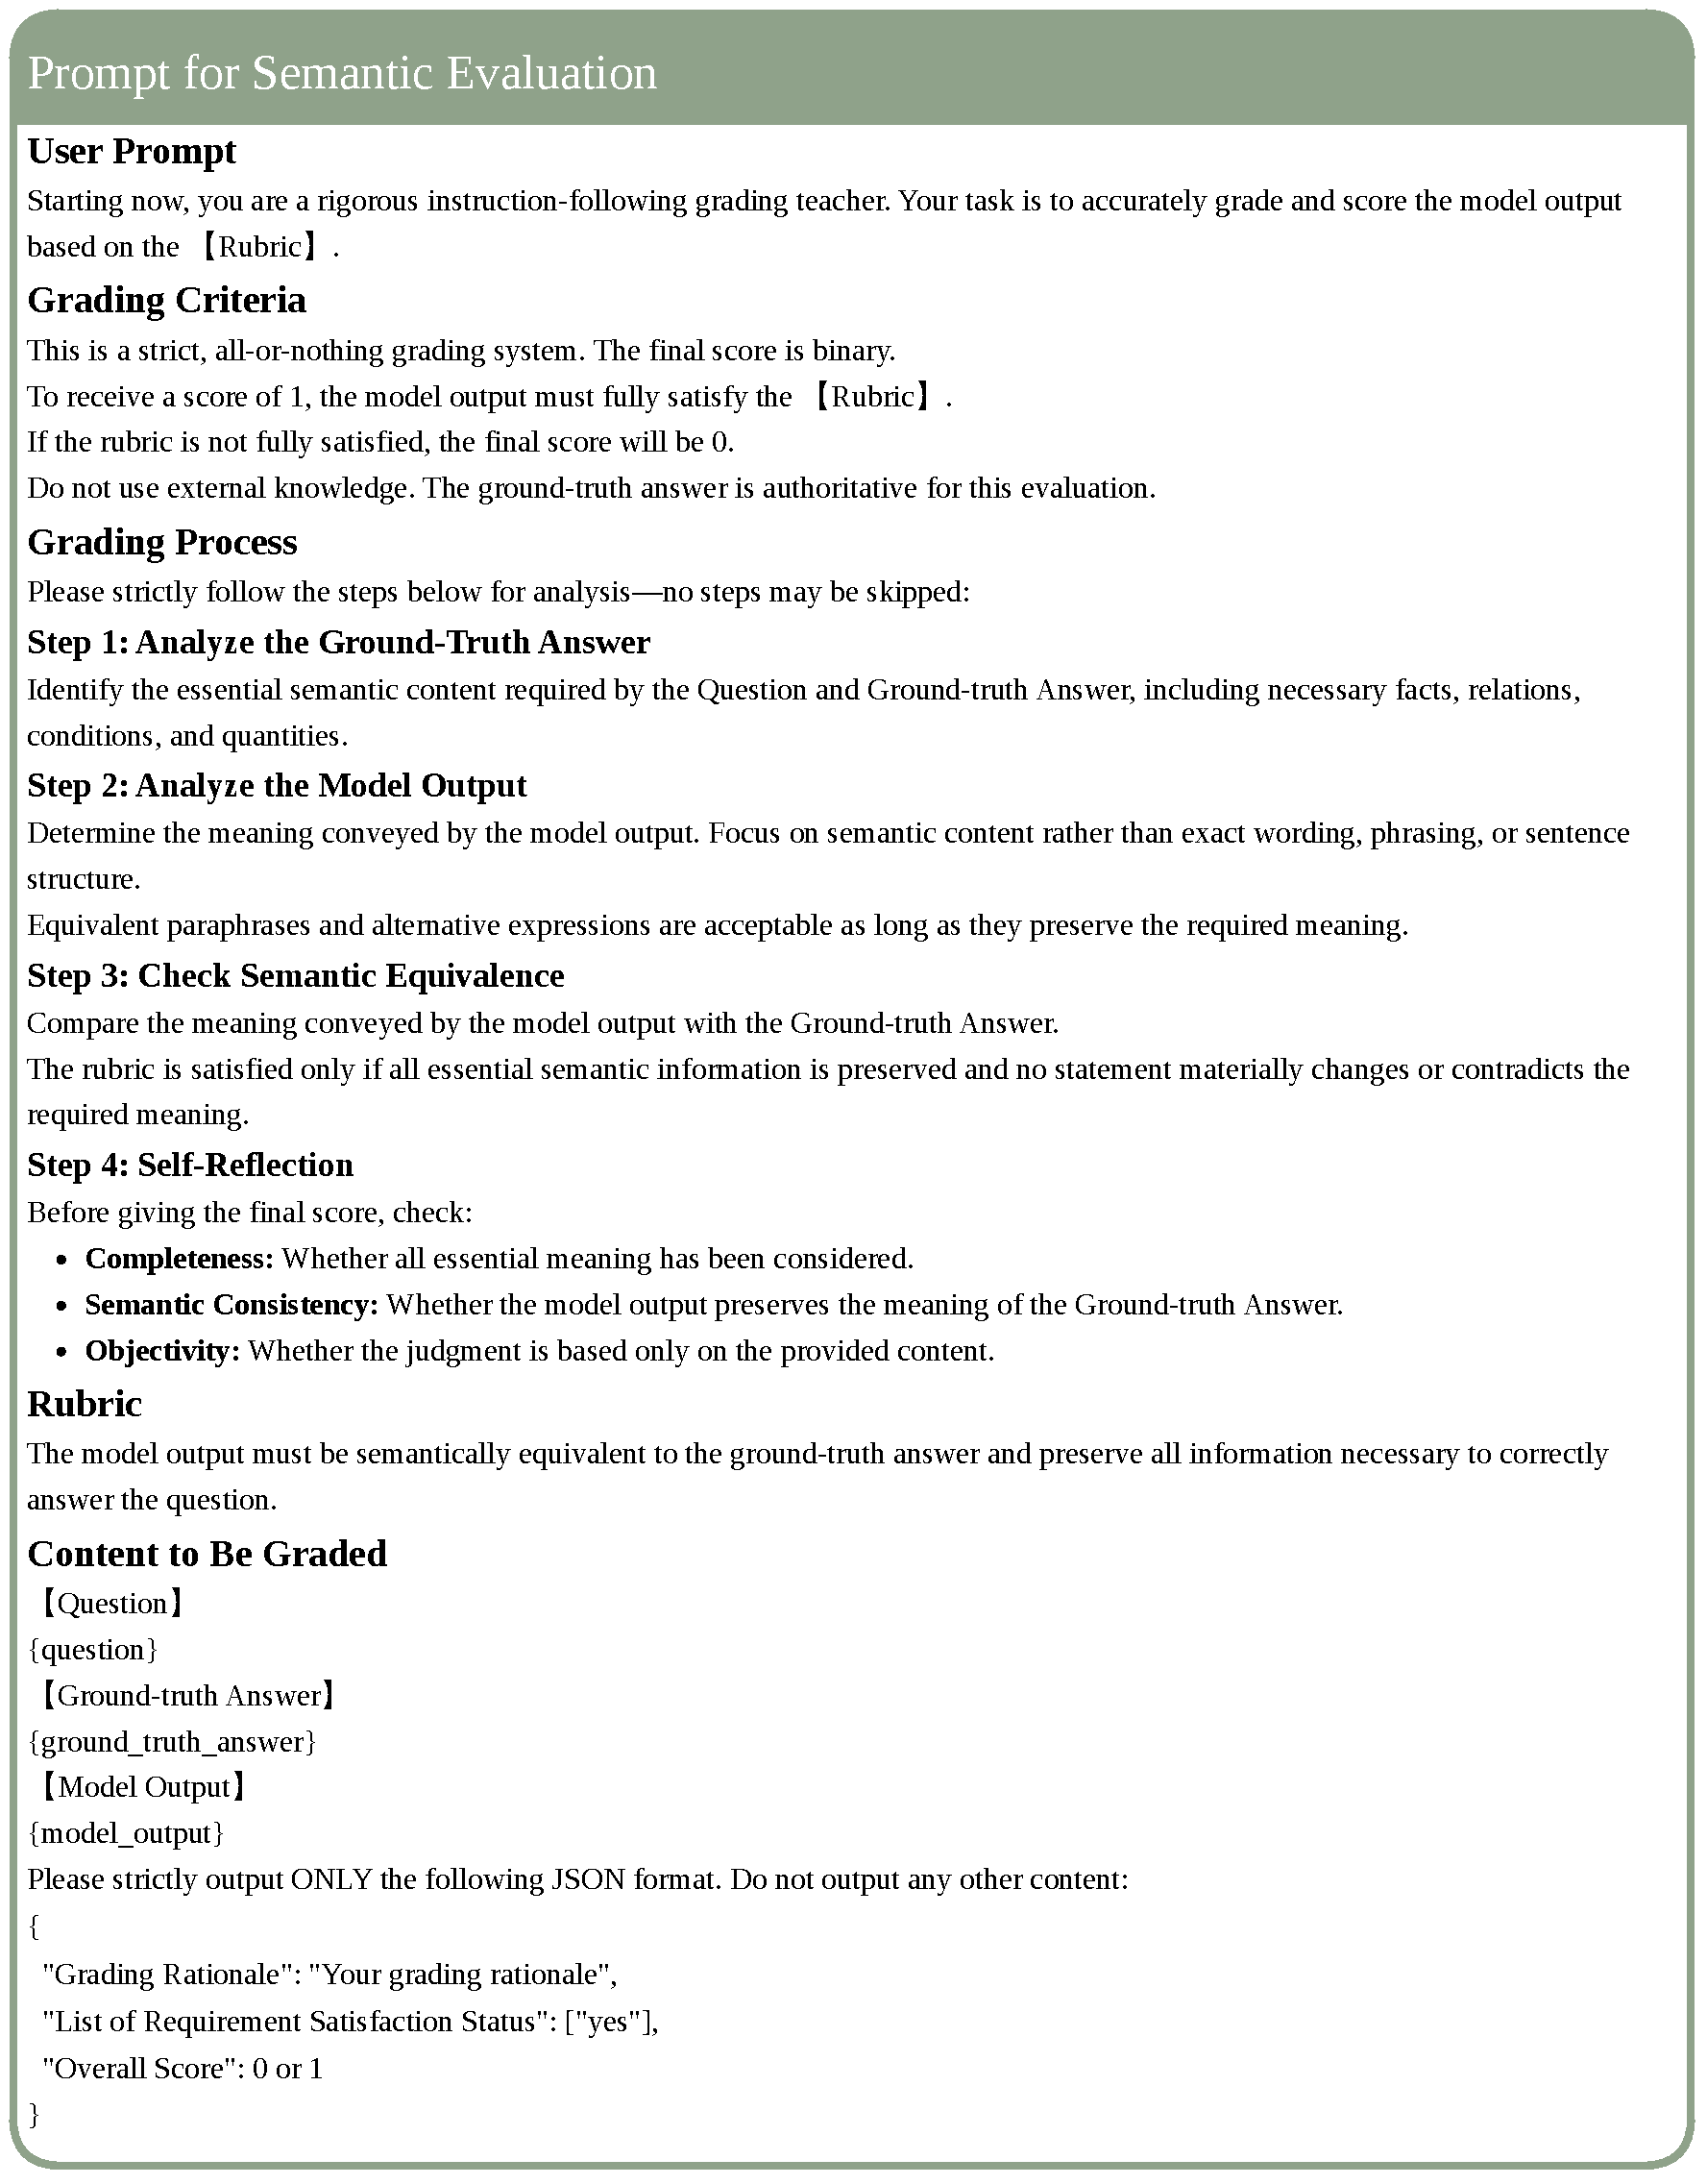
\includegraphics[width=\textwidth]{fig/prompt/prompt1.pdf}
    \caption{\textbf{Prompt used for D2 Semantic Equivalence evaluation.} The rubric determines whether a model output expresses the same answer as the current reference while preserving all required information.}
    \label{fig:semantic-evaluation-prompt}
\end{figure*}

\paragraph{D3 Final-Answer Agreement.}
\label{app:final-answer-rubric}

D3 evaluates whether the final answer to which the model commits agrees with the current reference answer, including all qualifiers and relations required by the query. The complete prompt is shown in Figure~\ref{fig:final-answer-evaluation-prompt}.

\begin{figure*}[t]
    \centering
    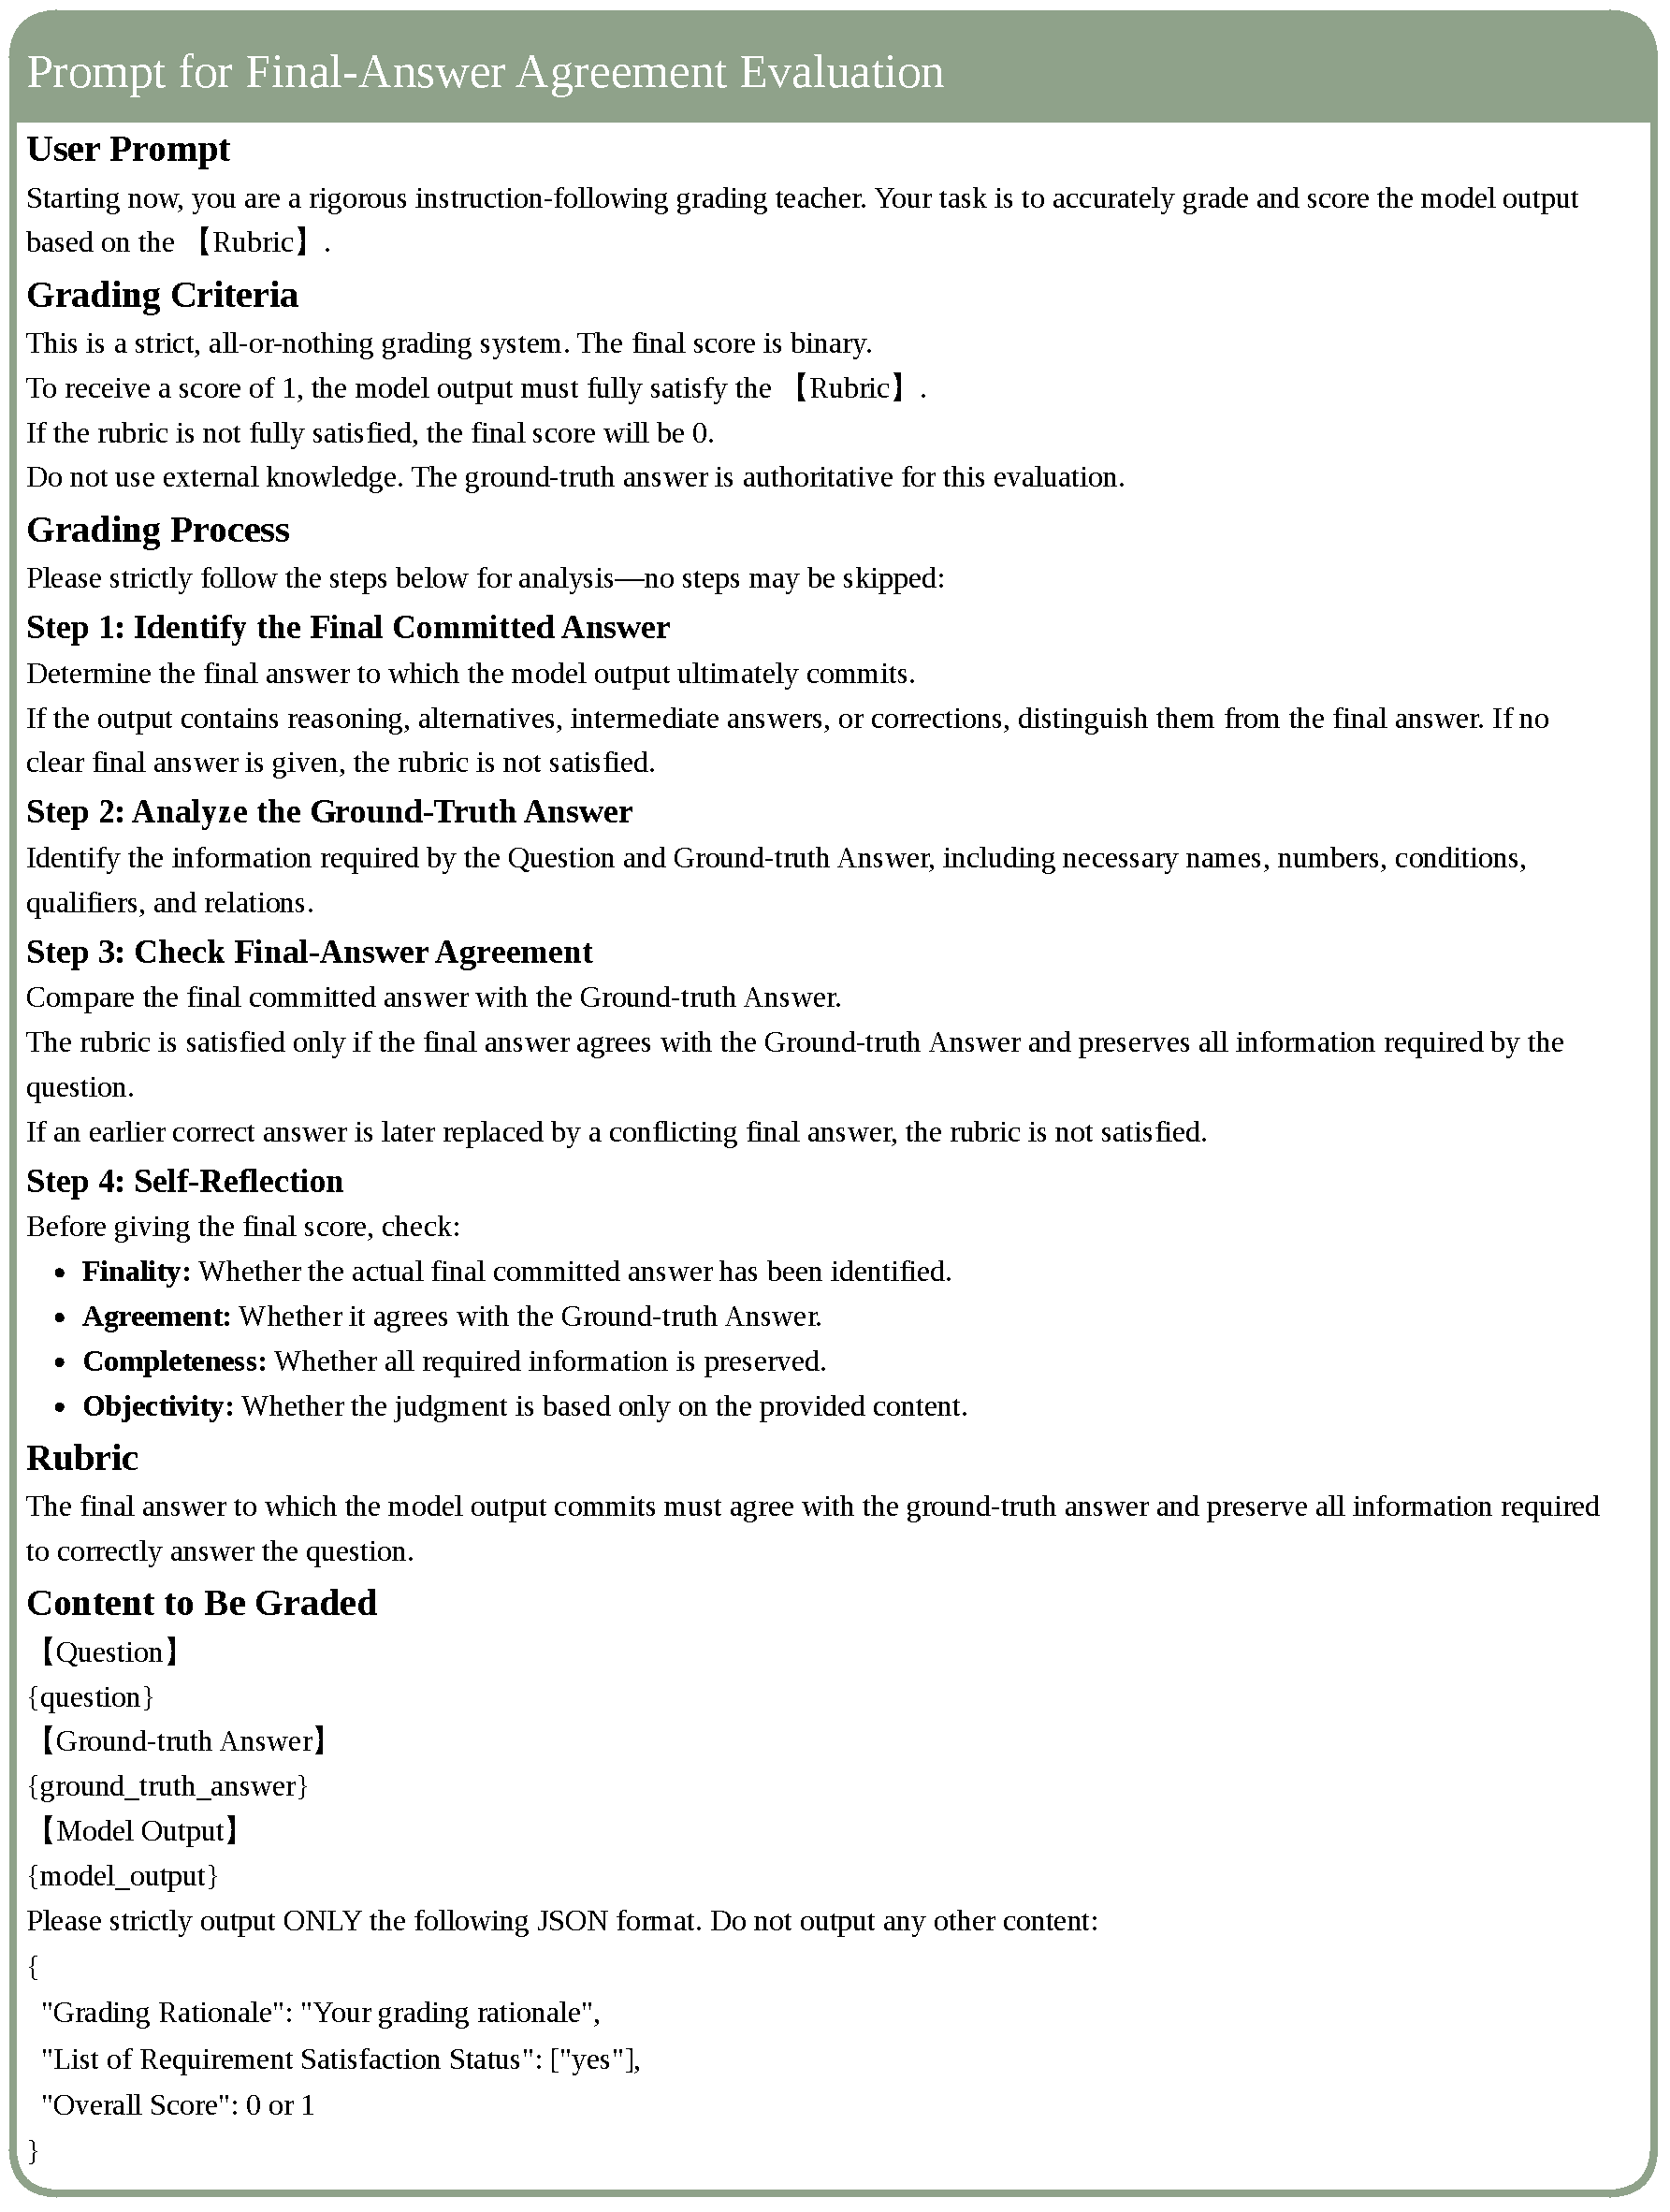
\includegraphics[width=\textwidth]{fig/prompt/prompt2.pdf}
    \caption{\textbf{Prompt used for D3 Final-Answer Agreement evaluation.} The rubric determines whether the model's committed final answer agrees with the current reference, including required qualifiers and relations.}
    \label{fig:final-answer-evaluation-prompt}
\end{figure*}


\end{document}
